% Options for packages loaded elsewhere
% Options for packages loaded elsewhere
\PassOptionsToPackage{unicode}{hyperref}
\PassOptionsToPackage{hyphens}{url}
\PassOptionsToPackage{dvipsnames,svgnames,x11names}{xcolor}
%
\documentclass[
  spanish,
  us-letterpaper,
  DIV=11,
  numbers=noendperiod]{scrreprt}
\usepackage{xcolor}
\usepackage{amsmath,amssymb}
\setcounter{secnumdepth}{5}
\usepackage{iftex}
\ifPDFTeX
  \usepackage[T1]{fontenc}
  \usepackage[utf8]{inputenc}
  \usepackage{textcomp} % provide euro and other symbols
\else % if luatex or xetex
  \usepackage{unicode-math} % this also loads fontspec
  \defaultfontfeatures{Scale=MatchLowercase}
  \defaultfontfeatures[\rmfamily]{Ligatures=TeX,Scale=1}
\fi
\usepackage{lmodern}
\ifPDFTeX\else
  % xetex/luatex font selection
\fi
% Use upquote if available, for straight quotes in verbatim environments
\IfFileExists{upquote.sty}{\usepackage{upquote}}{}
\IfFileExists{microtype.sty}{% use microtype if available
  \usepackage[]{microtype}
  \UseMicrotypeSet[protrusion]{basicmath} % disable protrusion for tt fonts
}{}
\makeatletter
\@ifundefined{KOMAClassName}{% if non-KOMA class
  \IfFileExists{parskip.sty}{%
    \usepackage{parskip}
  }{% else
    \setlength{\parindent}{0pt}
    \setlength{\parskip}{6pt plus 2pt minus 1pt}}
}{% if KOMA class
  \KOMAoptions{parskip=half}}
\makeatother
% Make \paragraph and \subparagraph free-standing
\makeatletter
\ifx\paragraph\undefined\else
  \let\oldparagraph\paragraph
  \renewcommand{\paragraph}{
    \@ifstar
      \xxxParagraphStar
      \xxxParagraphNoStar
  }
  \newcommand{\xxxParagraphStar}[1]{\oldparagraph*{#1}\mbox{}}
  \newcommand{\xxxParagraphNoStar}[1]{\oldparagraph{#1}\mbox{}}
\fi
\ifx\subparagraph\undefined\else
  \let\oldsubparagraph\subparagraph
  \renewcommand{\subparagraph}{
    \@ifstar
      \xxxSubParagraphStar
      \xxxSubParagraphNoStar
  }
  \newcommand{\xxxSubParagraphStar}[1]{\oldsubparagraph*{#1}\mbox{}}
  \newcommand{\xxxSubParagraphNoStar}[1]{\oldsubparagraph{#1}\mbox{}}
\fi
\makeatother

\usepackage{color}
\usepackage{fancyvrb}
\newcommand{\VerbBar}{|}
\newcommand{\VERB}{\Verb[commandchars=\\\{\}]}
\DefineVerbatimEnvironment{Highlighting}{Verbatim}{commandchars=\\\{\}}
% Add ',fontsize=\small' for more characters per line
\usepackage{framed}
\definecolor{shadecolor}{RGB}{241,243,245}
\newenvironment{Shaded}{\begin{snugshade}}{\end{snugshade}}
\newcommand{\AlertTok}[1]{\textcolor[rgb]{0.68,0.00,0.00}{#1}}
\newcommand{\AnnotationTok}[1]{\textcolor[rgb]{0.37,0.37,0.37}{#1}}
\newcommand{\AttributeTok}[1]{\textcolor[rgb]{0.40,0.45,0.13}{#1}}
\newcommand{\BaseNTok}[1]{\textcolor[rgb]{0.68,0.00,0.00}{#1}}
\newcommand{\BuiltInTok}[1]{\textcolor[rgb]{0.00,0.23,0.31}{#1}}
\newcommand{\CharTok}[1]{\textcolor[rgb]{0.13,0.47,0.30}{#1}}
\newcommand{\CommentTok}[1]{\textcolor[rgb]{0.37,0.37,0.37}{#1}}
\newcommand{\CommentVarTok}[1]{\textcolor[rgb]{0.37,0.37,0.37}{\textit{#1}}}
\newcommand{\ConstantTok}[1]{\textcolor[rgb]{0.56,0.35,0.01}{#1}}
\newcommand{\ControlFlowTok}[1]{\textcolor[rgb]{0.00,0.23,0.31}{\textbf{#1}}}
\newcommand{\DataTypeTok}[1]{\textcolor[rgb]{0.68,0.00,0.00}{#1}}
\newcommand{\DecValTok}[1]{\textcolor[rgb]{0.68,0.00,0.00}{#1}}
\newcommand{\DocumentationTok}[1]{\textcolor[rgb]{0.37,0.37,0.37}{\textit{#1}}}
\newcommand{\ErrorTok}[1]{\textcolor[rgb]{0.68,0.00,0.00}{#1}}
\newcommand{\ExtensionTok}[1]{\textcolor[rgb]{0.00,0.23,0.31}{#1}}
\newcommand{\FloatTok}[1]{\textcolor[rgb]{0.68,0.00,0.00}{#1}}
\newcommand{\FunctionTok}[1]{\textcolor[rgb]{0.28,0.35,0.67}{#1}}
\newcommand{\ImportTok}[1]{\textcolor[rgb]{0.00,0.46,0.62}{#1}}
\newcommand{\InformationTok}[1]{\textcolor[rgb]{0.37,0.37,0.37}{#1}}
\newcommand{\KeywordTok}[1]{\textcolor[rgb]{0.00,0.23,0.31}{\textbf{#1}}}
\newcommand{\NormalTok}[1]{\textcolor[rgb]{0.00,0.23,0.31}{#1}}
\newcommand{\OperatorTok}[1]{\textcolor[rgb]{0.37,0.37,0.37}{#1}}
\newcommand{\OtherTok}[1]{\textcolor[rgb]{0.00,0.23,0.31}{#1}}
\newcommand{\PreprocessorTok}[1]{\textcolor[rgb]{0.68,0.00,0.00}{#1}}
\newcommand{\RegionMarkerTok}[1]{\textcolor[rgb]{0.00,0.23,0.31}{#1}}
\newcommand{\SpecialCharTok}[1]{\textcolor[rgb]{0.37,0.37,0.37}{#1}}
\newcommand{\SpecialStringTok}[1]{\textcolor[rgb]{0.13,0.47,0.30}{#1}}
\newcommand{\StringTok}[1]{\textcolor[rgb]{0.13,0.47,0.30}{#1}}
\newcommand{\VariableTok}[1]{\textcolor[rgb]{0.07,0.07,0.07}{#1}}
\newcommand{\VerbatimStringTok}[1]{\textcolor[rgb]{0.13,0.47,0.30}{#1}}
\newcommand{\WarningTok}[1]{\textcolor[rgb]{0.37,0.37,0.37}{\textit{#1}}}

\usepackage{longtable,booktabs,array}
\usepackage{calc} % for calculating minipage widths
% Correct order of tables after \paragraph or \subparagraph
\usepackage{etoolbox}
\makeatletter
\patchcmd\longtable{\par}{\if@noskipsec\mbox{}\fi\par}{}{}
\makeatother
% Allow footnotes in longtable head/foot
\IfFileExists{footnotehyper.sty}{\usepackage{footnotehyper}}{\usepackage{footnote}}
\makesavenoteenv{longtable}
\usepackage{graphicx}
\makeatletter
\newsavebox\pandoc@box
\newcommand*\pandocbounded[1]{% scales image to fit in text height/width
  \sbox\pandoc@box{#1}%
  \Gscale@div\@tempa{\textheight}{\dimexpr\ht\pandoc@box+\dp\pandoc@box\relax}%
  \Gscale@div\@tempb{\linewidth}{\wd\pandoc@box}%
  \ifdim\@tempb\p@<\@tempa\p@\let\@tempa\@tempb\fi% select the smaller of both
  \ifdim\@tempa\p@<\p@\scalebox{\@tempa}{\usebox\pandoc@box}%
  \else\usebox{\pandoc@box}%
  \fi%
}
% Set default figure placement to htbp
\def\fps@figure{htbp}
\makeatother


% definitions for citeproc citations
\NewDocumentCommand\citeproctext{}{}
\NewDocumentCommand\citeproc{mm}{%
  \begingroup\def\citeproctext{#2}\cite{#1}\endgroup}
\makeatletter
 % allow citations to break across lines
 \let\@cite@ofmt\@firstofone
 % avoid brackets around text for \cite:
 \def\@biblabel#1{}
 \def\@cite#1#2{{#1\if@tempswa , #2\fi}}
\makeatother
\newlength{\cslhangindent}
\setlength{\cslhangindent}{1.5em}
\newlength{\csllabelwidth}
\setlength{\csllabelwidth}{3em}
\newenvironment{CSLReferences}[2] % #1 hanging-indent, #2 entry-spacing
 {\begin{list}{}{%
  \setlength{\itemindent}{0pt}
  \setlength{\leftmargin}{0pt}
  \setlength{\parsep}{0pt}
  % turn on hanging indent if param 1 is 1
  \ifodd #1
   \setlength{\leftmargin}{\cslhangindent}
   \setlength{\itemindent}{-1\cslhangindent}
  \fi
  % set entry spacing
  \setlength{\itemsep}{#2\baselineskip}}}
 {\end{list}}
\usepackage{calc}
\newcommand{\CSLBlock}[1]{\hfill\break\parbox[t]{\linewidth}{\strut\ignorespaces#1\strut}}
\newcommand{\CSLLeftMargin}[1]{\parbox[t]{\csllabelwidth}{\strut#1\strut}}
\newcommand{\CSLRightInline}[1]{\parbox[t]{\linewidth - \csllabelwidth}{\strut#1\strut}}
\newcommand{\CSLIndent}[1]{\hspace{\cslhangindent}#1}

\ifLuaTeX
\usepackage[bidi=basic]{babel}
\else
\usepackage[bidi=default]{babel}
\fi
% get rid of language-specific shorthands (see #6817):
\let\LanguageShortHands\languageshorthands
\def\languageshorthands#1{}


\setlength{\emergencystretch}{3em} % prevent overfull lines

\providecommand{\tightlist}{%
  \setlength{\itemsep}{0pt}\setlength{\parskip}{0pt}}



 


\KOMAoption{captions}{tableheading}
\makeatletter
\@ifpackageloaded{tcolorbox}{}{\usepackage[skins,breakable]{tcolorbox}}
\@ifpackageloaded{fontawesome5}{}{\usepackage{fontawesome5}}
\definecolor{quarto-callout-color}{HTML}{909090}
\definecolor{quarto-callout-note-color}{HTML}{0758E5}
\definecolor{quarto-callout-important-color}{HTML}{CC1914}
\definecolor{quarto-callout-warning-color}{HTML}{EB9113}
\definecolor{quarto-callout-tip-color}{HTML}{00A047}
\definecolor{quarto-callout-caution-color}{HTML}{FC5300}
\definecolor{quarto-callout-color-frame}{HTML}{acacac}
\definecolor{quarto-callout-note-color-frame}{HTML}{4582ec}
\definecolor{quarto-callout-important-color-frame}{HTML}{d9534f}
\definecolor{quarto-callout-warning-color-frame}{HTML}{f0ad4e}
\definecolor{quarto-callout-tip-color-frame}{HTML}{02b875}
\definecolor{quarto-callout-caution-color-frame}{HTML}{fd7e14}
\makeatother
\makeatletter
\@ifpackageloaded{bookmark}{}{\usepackage{bookmark}}
\makeatother
\makeatletter
\@ifpackageloaded{caption}{}{\usepackage{caption}}
\AtBeginDocument{%
\ifdefined\contentsname
  \renewcommand*\contentsname{Tabla de contenidos}
\else
  \newcommand\contentsname{Tabla de contenidos}
\fi
\ifdefined\listfigurename
  \renewcommand*\listfigurename{Listado de Figuras}
\else
  \newcommand\listfigurename{Listado de Figuras}
\fi
\ifdefined\listtablename
  \renewcommand*\listtablename{Listado de Tablas}
\else
  \newcommand\listtablename{Listado de Tablas}
\fi
\ifdefined\figurename
  \renewcommand*\figurename{Figura}
\else
  \newcommand\figurename{Figura}
\fi
\ifdefined\tablename
  \renewcommand*\tablename{Tabla}
\else
  \newcommand\tablename{Tabla}
\fi
}
\@ifpackageloaded{float}{}{\usepackage{float}}
\floatstyle{ruled}
\@ifundefined{c@chapter}{\newfloat{codelisting}{h}{lop}}{\newfloat{codelisting}{h}{lop}[chapter]}
\floatname{codelisting}{Listado}
\newcommand*\listoflistings{\listof{codelisting}{Listado de Listados}}
\usepackage{amsthm}
\theoremstyle{definition}
\newtheorem{definition}{Definición}[chapter]
\theoremstyle{plain}
\newtheorem{theorem}{Teorema}[chapter]
\theoremstyle{remark}
\AtBeginDocument{\renewcommand*{\proofname}{Prueba}}
\newtheorem*{remark}{Observación}
\newtheorem*{solution}{Solución}
\newtheorem{refremark}{Observación}[chapter]
\newtheorem{refsolution}{Solución}[chapter]
\makeatother
\makeatletter
\makeatother
\makeatletter
\@ifpackageloaded{caption}{}{\usepackage{caption}}
\@ifpackageloaded{subcaption}{}{\usepackage{subcaption}}
\makeatother
\usepackage{bookmark}
\IfFileExists{xurl.sty}{\usepackage{xurl}}{} % add URL line breaks if available
\urlstyle{same}
\hypersetup{
  pdftitle={Estimación de la temperatura con la ecuación del Bio-Calor usando DeepONet},
  pdfauthor={Francisco Damián Escobar Candelaria; Yofre Hernán García Gómez},
  pdflang={es},
  colorlinks=true,
  linkcolor={blue},
  filecolor={Maroon},
  citecolor={Blue},
  urlcolor={Blue},
  pdfcreator={LaTeX via pandoc}}


\title{Estimación de la temperatura con la ecuación del Bio-Calor usando
DeepONet}
\author{Francisco Damián Escobar Candelaria \and Yofre Hernán García
Gómez}
\date{2025-04-21}
\begin{document}
\maketitle

\renewcommand*\contentsname{Tabla de contenidos}
{
\hypersetup{linkcolor=}
\setcounter{tocdepth}{2}
\tableofcontents
}

\bookmarksetup{startatroot}

\chapter*{Resumen}\label{resumen}
\addcontentsline{toc}{chapter}{Resumen}

\markboth{Resumen}{Resumen}

Este trabajo explora el uso de DeepONet para resolver ecuaciones
diferenciales parciales, aplicándola a la estimación de temperatura en
tejidos biológicos mediante la ecuación del bio-calor, en contextos
clínicos como la hipertermia oncológica.

Se comparó el desempeño de DeepONet frente a un método numérico clásico,
como Crank-Nicolson, evaluando precisión mediante métricas de error. La
red neuronal fue entrenada para resolver la EDP del Bio-Calor
simplificandola de manera que no se tuviera en cuenta la fuente
metabólica de calor \(Q\).

Los resultados muestran que DeepONet puede aproximar la solución
eficazmente en distintos tiempos, con ventajas de generalización
respecto a redes PINN convencionales, posicionándose como una
herramienta prometedora en el modelado térmico biomédico.

\bookmarksetup{startatroot}

\chapter{Introducción}\label{introducciuxf3n}

El uso de redes neuronales en la resolución de ecuaciones diferenciales
parciales (EDPs) ha ganado relevancia en la última década gracias al
desarrollo de técnicas que integran principios físicos en el
entrenamiento de modelos. Este enfoque, conocido como redes neuronales
informadas por la física (PINNs), ha demostrado ser especialmente útil
en situaciones donde la disponibilidad de datos es limitada y donde las
leyes físicas subyacentes pueden ser incorporadas como restricciones en
la función de pérdida (\citeproc{ref-karniadakis2021}{George Em
Karniadakis 2021}). En este trabajo se explora una variante más
reciente: DeepONet, una arquitectura diseñada para aprender operadores
funcionales, y su aplicación en la estimación de temperatura en tejidos
biológicos mediante la ecuación del Bio-Calor.

La ecuación del Bio-Calor fue propuesta por Pennes en 1948 con el
objetivo de modelar la transferencia de calor en tejidos vivos,
considerando los efectos de conducción térmica, metabolismo y perfusión
sanguínea (\citeproc{ref-pennes1948}{Pennes 1948}). Este modelo ha sido
ampliamente utilizado en aplicaciones clínicas como la hipertermia
terapéutica, una técnica que consiste en elevar localmente la
temperatura del tejido para mejorar la eficacia de tratamientos
oncológicos (\citeproc{ref-nci2021}{Instituto Nacional del Cáncer
2021}). Sin embargo, debido a la complejidad de las condiciones
fisiológicas y a las propiedades variables de los tejidos, su resolución
analítica es inviable, y las aproximaciones numéricas, como el método de
Crank-Nicolson, se vuelven indispensables.

En este contexto, surge la oportunidad de aplicar DeepONet como una
alternativa innovadora. A diferencia de una PINN tradicional, que se
entrena para resolver una instancia específica de una EDP, DeepONet
aprende un operador que puede generalizar a nuevas condiciones de
frontera o iniciales sin requerir reentrenamiento
(\citeproc{ref-deepxde}{Lu, Meng, et~al. 2021}). Esta característica
resulta de gran valor en aplicaciones médicas donde las condiciones
pueden variar entre pacientes o incluso durante un mismo procedimiento.
Además, el modelo puede ser entrenado sobre una base de soluciones
simuladas, lo que reduce la necesidad de datos experimentales, difíciles
y costosos de obtener en contextos clínicos
(\citeproc{ref-karniadakis2021}{George Em Karniadakis 2021}).

El presente trabajo tiene como objetivo comparar la precisión y
eficiencia de DeepONet con el método numérico clásico de Crank-Nicolson
en la estimación de temperatura sobre un dominio bidimensional. Para
ello, se implementó un modelo basado en la versión adimensionalizada de
la ecuación del Bio-Calor, y se utilizó la biblioteca DeepXDE para su
entrenamiento (\citeproc{ref-deepxde}{Lu, Meng, et~al. 2021}).
Posteriormente, se evaluaron métricas como el error medio absoluto (MAE)
y el error máximo absoluto (MaxAE), y se analizaron las predicciones
visualmente frente a referencias obtenidas por Alessio Borgi
(\citeproc{ref-medical_rep}{2023}), con resultados prometedores.

La combinación de eficiencia, capacidad de generalización y adecuación a
condiciones reales posiciona a DeepONet como una alternativa poderosa
frente a métodos clásicos. Esta tesis busca sentar las bases para
diversificar su uso en escenarios variados e incentivar su uso en la
solución de operadores. Así, el trabajo contribuye a la creciente
tendencia de aplicar inteligencia artificial en el ámbito médico con
fundamentos sólidos en física matemática.

\bookmarksetup{startatroot}

\chapter{Objetivos}\label{objetivos}

\section{Objetivo general}\label{objetivo-general}

Comparar la aproximación numérica de la solución de una Ecuación
Diferencial Parcial (EDP) obtenida del uso de una red neuronal con
arquitectura DeepONet, con aproximaciones numéricas obtenidas con
métodos numéricos clásicos, en el contexto de un estudio médico basado
en la EDP del Bio-Calor, utilizando métricas de error relevantes para
evaluar su desempeño.

\section{Objetivos específicos}\label{objetivos-especuxedficos}

\begin{enumerate}
\def\labelenumi{\arabic{enumi}.}
\item
  Comprender y adaptar el uso de las PINNs para la resolución de PDEs y
  ODEs así como sus aplicaciones multidisciplinarias.
\item
  Explorar el uso de DeepONet como alternativa a las PINNs clásicas y
  determinar tanto ventajas como desventajas de su implementación.
\item
  Evaluar y contrastar la eficacia de la arquitectura de red neuronal
  artificial DeepONet con un método numérico de referencia, como el
  método de Crank Nickolson.
\item
  Reconocer la dificultades que se tiene al momento de implementar un
  modelo de red neuronal en un lenguaje de programación como Python.
\end{enumerate}

\part{Preliminares}

\chapter{Ecuaciones diferenciales
parciales}\label{ecuaciones-diferenciales-parciales}

Las ecuaciones diferenciales parciales (EDPs), al igual que las
ecuaciones diferenciales ordinarias (EDOs), se clasifican en lineales y
no lineales. De forma análoga a una EDO lineal, la variable dependiente
y sus derivadas parciales en una EDP lineal se elevan únicamente a la
primera potencia (\citeproc{ref-zill2008}{Zill y Cullen 2008}).

\section{Ecuación diferencial parcial
lineal}\label{ecuaciuxf3n-diferencial-parcial-lineal}

Si dejamos que \(u\) denote la variable dependiente y que \(x\) e \(y\)
representen las variables independientes, entonces la forma general de
una \textbf{ecuación diferencial parcial lineal de segundo orden} está
dada por:

\begin{equation}\phantomsection\label{eq-LPDE}{
A \dfrac{\partial^2 u}{\partial x^2} + B \dfrac{\partial^2 u}{\partial x \, \partial y} + C \dfrac{\partial^2 u}{\partial y^2} + D \dfrac{\partial u}{\partial x} + E \dfrac{\partial u}{\partial y} + F u = G,
}\end{equation}

donde los coeficientes \(A, B, C, \dots, G\) son funciones de \(x\) e
\(y\). Cuando \(G(x, y) = 0\), la ecuación \ref{eq-LPDE} se denomina
\textbf{homogénea}; de lo contrario, es \textbf{no homogénea}. Por
ejemplo, las ecuaciones lineales:

\[
\dfrac{\partial^2 u}{\partial x^2} + \dfrac{\partial^2 u}{\partial y^2} = 0 \quad\text{y} \quad \dfrac{\partial^2 u}{\partial x^2} - \dfrac{\partial u}{\partial y} = x y
\] son homogénea y no homogénea, respectivamente.

\section{Solucion de una PDE}\label{solucion-de-una-pde}

Una \textbf{solución} de una ecuación diferencial parcial es una función
\(u(x, y)\) de dos variables independientes que posee todas las
derivadas parciales que aparecen en la ecuación y que satisface dicha
ecuación en alguna región del plano \(xy\).

No es lo habitual examinar los procedimientos para encontrar
\textbf{soluciones generales} de ecuaciones diferenciales parciales
lineales. No solo porque suele ser difícil obtener una solución general
de una EDP lineal de segundo orden, sino que una solución general
generalmente no es tan útil en aplicaciones prácticas. Por lo tanto, el
enfoque común es el de encontrar \textbf{soluciones particulares} de
algunas de las EDPs lineales más importantes, es decir, ecuaciones que
aparecen en muchas aplicaciones.

\section{Separación de variables}\label{separaciuxf3n-de-variables}

Aunque existen varios métodos que pueden intentarse para encontrar
soluciones particulares de una EDP lineal, uno de los métodos más
comunes se llama \textbf{método de separación de variables}. En este
método buscamos una solución particular de la forma de un
\emph{producto} de una función de \(x\) y una función de \(y\):

\[
u(x, y) = X(x)Y(y).
\]

Con esta suposición, \emph{a veces} es posible reducir una EDP lineal en
dos variables a dos ecuaciones diferenciales ordinarias (ODEs). Para
este fin, observamos que:

\[
\dfrac{\partial u}{\partial x} = X'Y, \quad
\dfrac{\partial u}{\partial y} = XY', \quad
\dfrac{\partial^2 u}{\partial x^2} = X''Y, \quad
\dfrac{\partial^2 u}{\partial y^2} = XY'',
\]

donde las comillas (\emph{primes}) denotan derivación ordinaria.

\section{Principio de
superposición}\label{principio-de-superposiciuxf3n}

\begin{theorem}[]\protect\hypertarget{thm-superposition}{}\label{thm-superposition}

Si \(u_1 , u_2 , \dots , u_k\) son soluciones de una ecuación
diferencial parcial lineal homogénea, entonces la combinación lineal \[
u = c_1u_1 + c_2u_2 + \dots + c_ku_k
\] donde las \(c_i, i=1,2,\dots,k\) son constantes. Es también una
solución.

\end{theorem}

El teorema \ref{thm-superposition} se puede entender como: \emph{siempre
que tengamos un conjunto infinito de soluciones
\(u_1, u_2, u_3, \ldots\) de una ecuación lineal homogénea, podemos
construir otra solución \(u\) mediante la serie infinita}:

\[  
u = \sum_{k=1}^{\infty} c_k u_k,  
\]\\
donde las constantes \(c_i\), con \(i = 1, 2, \ldots\), son
coeficientes.

\section{Clasificación de
ecuaciones}\label{clasificaciuxf3n-de-ecuaciones}

Una ecuación diferencial parcial lineal de segundo orden con dos
variables independientes y coeficientes constantes puede clasificarse en
uno de tres tipos. Esta clasificación depende únicamente de los
coeficientes de las derivadas de segundo orden. Por supuesto, asumimos
que al menos uno de los coeficientes \(A\), \(B\) o \(C\) es distinto de
cero.

\begin{definition}[]\protect\hypertarget{def-PDEs-classes}{}\label{def-PDEs-classes}

La ecuación diferencial parcial lineal de segundo orden \[
A \dfrac{\partial^2 u}{\partial x^2} + B \dfrac{\partial^2 u}{\partial x \, \partial y} + C \dfrac{\partial^2 u}{\partial y^2} + D \dfrac{\partial u}{\partial x} + E \dfrac{\partial u}{\partial y} + F u = 0,
\] donde \(A,B,C,D,F\) son constantes reales, se dice que es:

\begin{itemize}
\tightlist
\item
  \textbf{Hiperbólica} si \(\quad B^2-4AC>0\),
\item
  \textbf{Parabólica} si \(\quad B^2-4AC=0\),
\item
  \textbf{Elíptica} si \(\quad B^2-4AC<0\).
\end{itemize}

\end{definition}

\chapter{Problemas de valores en la
frontera}\label{problemas-de-valores-en-la-frontera}

Si, por ejemplo, \(u(x, t)\) es una solución de una EDP, donde \(x\)
representa una dimensión espacial y \(t\) representa el tiempo, entonces
es posible prescribir el valor de \(u\), o
\(\frac{\partial u}{\partial x}\), o una combinación lineal de \(u\) y
\(\frac{\partial u}{\partial x}\) en un valor \(x\) especificado, así
como prescribir \(u\) y \(\frac{\partial u}{\partial t}\) en un instante
dado \(t\) (normalmente, \(t=0\)). En otras palabras, un \emph{problema
de valores en la frontera} puede consistir en una EDP, junto con
\emph{condiciones de frontera} y \emph{condiciones iniciales}
(\citeproc{ref-zill2008}{Zill y Cullen 2008}).

\section{Ecuaciones clásicas}\label{ecuaciones-cluxe1sicas}

Aplicar el método de separación de variables para encontrar soluciones
en forma de producto es muy común con las siguientes \emph{ecuaciones
clásicas} de la física matemática:

\begin{equation}\phantomsection\label{eq-heat}{  
k\frac{\partial^2 u}{\partial x^2} = \frac{\partial u}{\partial t}, \quad k > 0  
}\end{equation}

\begin{equation}\phantomsection\label{eq-wave}{  
\alpha^2 \frac{\partial^2 u}{\partial x^2} = \frac{\partial^2 u}{\partial t^2}  
}\end{equation}

\begin{equation}\phantomsection\label{eq-laplace}{  
\frac{\partial^2 u}{\partial x^2} + \frac{\partial^2 u}{\partial y^2} = 0  
}\end{equation}

o variantes ligeras de estas ecuaciones. Las EDPs \ref{eq-heat},
\ref{eq-wave} y \ref{eq-laplace} se conocen, respectivamente, como la
\emph{ecuación del calor unidimensional}, la \emph{ecuación de onda
unidimensional} y la \emph{forma bidimensional de la ecuación de
Laplace}. El término ``unidimensional'' en el caso de las ecuaciones
\ref{eq-heat} y \ref{eq-wave} se refiere al hecho de que \(x\) denota
una variable espacial, mientras que \(t\) representa el tiempo;
``bidimensional'' en \ref{eq-laplace} significa que tanto \(x\) como
\(y\) son variables espaciales. Si comparas
\ref{eq-heat}-\ref{eq-laplace} con la forma lineal en la
Definición~\ref{def-PDEs-classes} (donde \(t\) juega el papel del
símbolo \(y\)), observarás que la ecuación del calor \ref{eq-heat} es
parabólica, la ecuación de onda \ref{eq-wave} es hiperbólica y la
ecuación de Laplace \ref{eq-laplace} es elíptica.

\begin{figure}

\begin{minipage}{0.50\linewidth}

\centering{

\pandocbounded{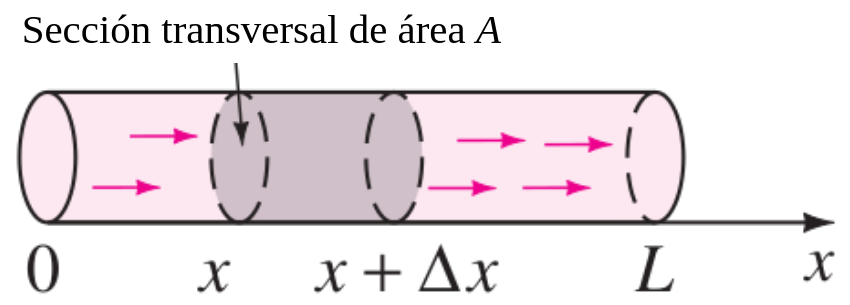
\includegraphics[keepaspectratio]{images/cross-section.png}}

}

\subcaption{\label{fig-1D-heat}Flujo de calor unidimensional.}

\end{minipage}%
%
\begin{minipage}{0.50\linewidth}

\centering{

\pandocbounded{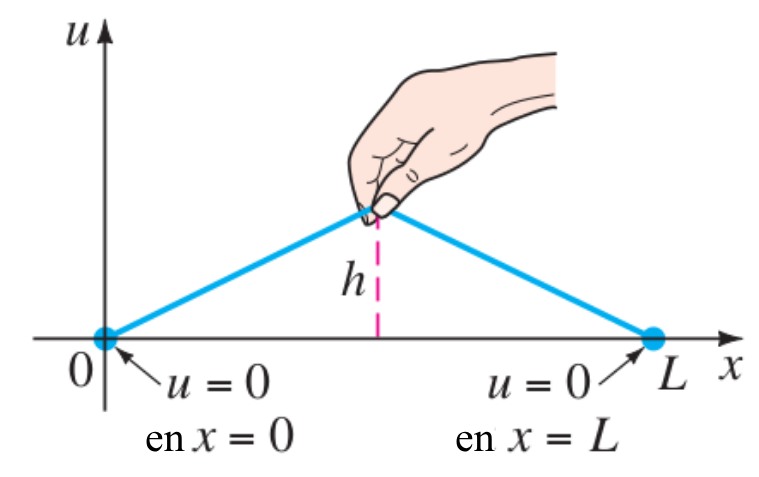
\includegraphics[keepaspectratio]{images/wave-eq.png}}

}

\subcaption{\label{fig-wave-exmpl}Cuerda tensada.}

\end{minipage}%

\caption{\label{fig-examples-eqs}Aplicaciones de las ecuaciones
\ref{eq-heat} y \ref{eq-wave} (\citeproc{ref-zill2008}{Zill y Cullen
2008}).}

\end{figure}%

\section{Condiciones iniciales}\label{condiciones-iniciales}

Dado que las soluciones de las ecuaciones \ref{eq-heat} y \ref{eq-wave}
dependen del tiempo \(t\), es posible especificar lo que ocurre en
\(t = 0\); es decir, establecer \textbf{condiciones iniciales (CI)}. Si
\(f(x)\) representa la distribución inicial de temperatura en la varilla
mostrada en la Figura~\ref{fig-1D-heat}, entonces una solución
\(u(x, t)\) de \ref{eq-heat} debe satisfacer la condición inicial única
\(u(x, 0) = f(x), \quad 0 < x < L\).

Por otro lado, para una cuerda vibrante podemos especificar tanto su
desplazamiento inicial (o forma) \(f(x)\) como su velocidad inicial
\(g(x)\). En términos matemáticos, buscamos una función \(u(x, t)\) que
satisfaga \ref{eq-wave} y las dos condiciones iniciales:
\begin{equation}\phantomsection\label{eq-initail-cond}{
u(x, 0) = f(x), \quad \left. \frac{\partial u}{\partial t} \right|_{t=0} = g(x), \quad 0 < x < L.
}\end{equation}

Por ejemplo, la cuerda podría ser tensada, como se muestra en la
Figura~\ref{fig-wave-exmpl}, y liberada desde el reposo \((g(x)=0)\).

\section{Condiciones de frontera}\label{condiciones-de-frontera}

La cuerda en la Figura~\ref{fig-wave-exmpl} está fija al eje \(x\) en
\(x=0\) y \(x=L\) para todos los tiempos. Ésto se interpreta a través de
dos \textbf{condiciones de frontera (CF):} \[
u(0,t) = 0, \quad u(L,t)=0, \quad t>0.
\] En éste contexto la función \(f\) en la ec~\ref{eq-initail-cond} es
continua y, en consecuencia, \(f(0)=0\) y \(f(L)=0\). En general,
existen tres tipos de condiciones de frontera asociadas con las
ecuaciones \ref{eq-heat}, \ref{eq-wave} y \ref{eq-laplace}. En la
frontera es posible especificar los valores de \emph{una} de las
siguientes:

\[
\text{(i)}\quad u, \qquad \text{(ii)}\quad \dfrac{\partial u}{\partial n},\qquad \text{or}\qquad \text{(iii)}\quad \dfrac{\partial u}{\partial n} + hu,\quad \text{con $h$ constante.}
\]

Aquí \(\frac{\partial u}{\partial n}\) denota la derivada normal de
\(u\) (la derivada de \(u\) en dirección perpendicular a la frontera).
Una condición de frontera del primer tipo (i) es llamada
\textbf{condición de Dirichlet}; una condición de frontera del segundo
tipo (ii) es llamada \textbf{condición de Neumann}; y una condición de
frontera del tercer tipo (iii) es conocida como \textbf{condición de
Robin}. Por ejemplo, para \(t>0\) una condición típica al extremo
derecho de la varilla de la Figura~\ref{fig-1D-heat} puede ser:

\begin{align*}
  \text{(i)}'   &\quad u(L,t) = u_0, \text{  con } u_0 \text{ constante} \\ \\
  \text{(ii)}'  &\quad \left. \dfrac{\partial u}{\partial x} \right|_{x=L} = 0 \\ \\
  \text{(iii)}' &\quad \left. \dfrac{\partial u}{\partial x} \right|_{x=L} = -h(u(L,t)-u_m),\text{  con } h>0 \text{ y } u_m \text{ constantes}
\end{align*}

La condición (i)' simplemente establece que el límite \(x=L\) se
mantiene, por algún medio, a una temperatura constante \(u_0\) durante
todo el tiempo \(t>0\). La condición (ii)' indica que el contorno
\(x=L\) está \emph{aislado}. Según la ley empírica de la transferencia
de calor, el flujo de calor a través del borde (es decir, la cantidad de
calor por unidad de área por unidad de tiempo conducida a través la
frontera) es proporcional al valor de la derivada normal
\(\frac{\partial u}{\partial n}\) de la temperatura \(u\). Por lo tanto,
cuando el límite \(x=L\) está aislado térmicamente, no fluye calor hacia
dentro ni hacia fuera de la varilla, por lo que \[
\left. \dfrac{\partial u}{\partial x} \right|_{x=L} = 0.
\]

Es posible interpretar (iii)' como que el calor se pierde del extremo
derecho de la varilla al estar en contacto con un medio, como el aire o
el agua, que se mantiene a temperatura constante. Según la ley de
enfriamiento de Newton, el flujo de calor hacia afuera de la varilla es
proporcional a la diferencia entre la temperatura \(u(L, t)\) en la
frontera y la temperatura \(u_m\) del medio circundante. Se observa que
si se pierde calor por el extremo izquierdo de la varilla, la condición
de contorno es \[
\left. \dfrac{\partial u}{\partial x} \right|_{x=0} = h(u(0,t)-u_m).
\] El cambio de signo respecto de (iii)' corresponde con el supuesto de
que la varilla está a una temperatura más alta que el medio que rodea
los extremos, de modo que \(u(0, t) > u_m\) y \(u(L, t) > u_m\). Para
\(x=0\) y \(x=L\), las pendientes \(u_x(0, t)\) y \(u_x(L, t)\) deben
ser positivas y negativas, respectivamente.

Por supuesto, en los extremos de la varilla se pueden especificar
diferentes condiciones al mismo tiempo. Por ejemplo, podríamos tener \[
\left. \dfrac{\partial u}{\partial x} \right|_{x=0} =0 \quad \text{y} \qquad u(L,t)=u_0, \quad t>0.
\]

\chapter{Problemas de valor inicial}\label{problemas-de-valor-inicial}

Las ecuaciones diferenciales son utilizadas para modelar problemas en
ciencia e ingeniería que implican el cambio de una variable con respecto
a otra. La mayoría de estos problemas requieren la solución de un
problema de valor inicial, es decir, la solución de una ecuación
diferencial que satisface una condición inicial dada.

En situaciones reales comunes, la ecuación diferencial que modela el
problema es demasiado compleja para resolverse con exactitud, y se
adopta uno de dos enfoques para aproximar la solución. El primer enfoque
consiste en modificar el problema simplificando la ecuación diferencial
a una que pueda resolverse con exactitud y luego utilizar la solución de
la ecuación simplificada para aproximar la solución del problema
original. El otro enfoque utiliza métodos para aproximar la solución del
problema original. Este es el enfoque más común porque los métodos de
aproximación proporcionan resultados más precisos e información de error
realista (\citeproc{ref-burden2011}{Burden y Faires 2010}).

\begin{tcolorbox}[enhanced jigsaw, breakable, titlerule=0mm, opacityback=0, left=2mm, toprule=.15mm, arc=.35mm, colbacktitle=quarto-callout-caution-color!10!white, toptitle=1mm, colback=white, title={Ejemplo}, leftrule=.75mm, bottomtitle=1mm, colframe=quarto-callout-caution-color-frame, bottomrule=.15mm, rightrule=.15mm, opacitybacktitle=0.6, coltitle=black]

El movimiento de un péndulo oscilante bajo ciertas suposiciones se
describe mediante la ecuación diferencial de segundo orden: \[
\dfrac{d^2 \theta}{d t^2} + \dfrac{g}{L} \sin{\theta} = 0 
\]

Donde \(L\) es la longitud del péndulo, \(g \approx 9.81 \frac{m}{s^2}\)
es la constante gravitacional terrestre y \(\theta\) es el ángulo que
forma el péndulo con la vertical. Si, además, especificamos la posición
del péndulo al inicio del movimiento, \(\theta(t_0) = \theta_{0}\) , y
su velocidad en ese punto, \(\theta'(t_0) = \theta'_0\). Tenemos un
\emph{problema de valor inicial}.

\end{tcolorbox}

Para dar una idea más clara acerca de los problemas de valor inicial
Burden y Faires (\citeproc{ref-burden2011}{2010}) brinda las siguientes
definiciones y teoremas:

\begin{definition}[]\protect\hypertarget{def-Lip-con}{}\label{def-Lip-con}

Se dice que una función \(f(t,y)\) satisface una \textbf{Condición de
Lipschitz} en la variable \(y\) en un conjunto
\(D \subset \mathbb{R}^2\) si existe una constante \(L>0\) tal que \[
|f(t,y_1) - f(t,y_2)| \leq L|y_1-y_2|
\]

donde \(f(t,y_1) \ \ \text{y} \ \ f(t,y_2)\) están en \(D\). La
constante \(L\) es llamada \textbf{constante de Lipschitz} para \(f\).

\end{definition}

\begin{definition}[]\protect\hypertarget{def-convex-set}{}\label{def-convex-set}

Se dice que un conjunto \(D \subset \mathbb{R}^2\) es \textbf{convexo}
si para cualesquiera \(f(t,y_1), f(t,y_2) \in D\), entonces
\(((1-\lambda)t_1 + \lambda t_2, (1-\lambda)y_1 + \lambda y_2)\) también
pertenece a \(D\) para cada \(\lambda \in[0,1]\).

\end{definition}

En términos geométricos, la Definición~\ref{def-convex-set} establece
que un conjunto es convexo siempre que, para cualesquiera dos puntos
dentro del conjunto, todo el segmento recto entre ellos también
pertenezca al conjunto Figura~\ref{fig-convx-set}.

\begin{figure}

\centering{

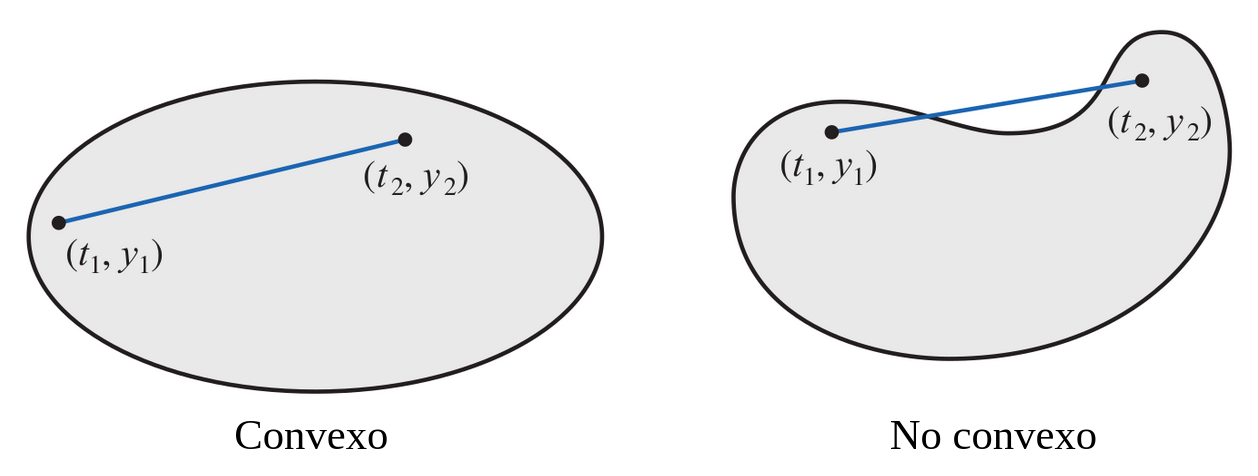
\includegraphics[width=6.25in,height=\textheight,keepaspectratio]{images/definition_5-2.png}

}

\caption{\label{fig-convx-set}Ejemplo geométrico de un conjunto
\emph{convexo} y \emph{no convexo} (\citeproc{ref-burden2011}{Burden y
Faires 2010}).}

\end{figure}%

\begin{theorem}[]\protect\hypertarget{thm-Lib-teo}{}\label{thm-Lib-teo}

Supongamos que \(f(t, y)\) está definida en un conjunto convexo
\(D \in \mathbb{R}^2\). Si existe una constante \(L > 0\) con
\begin{equation}\phantomsection\label{eq-Lib-teo}{
\left|\dfrac{\partial f}{\partial y}(t,y) \right| \leq L, \quad \text{para todo} \ \ (t,y)\in D,
}\end{equation}

entonces \(f\) satisface una condición de Lipschitz en \(D\) en la
variable \(y\) con una constante de Lipschitz \(L\).

\end{theorem}

Como se mostrará en el siguiente teorema, suele ser de gran interés
determinar si la función involucrada en un problema de valor inicial
satisface una condición de Lipschitz en su segunda variable, y la
condición \ref{eq-Lib-teo} suele ser más fácil de aplicar que la
definición. Cabe destacar, sin embargo, que el Teorema~\ref{thm-Lib-teo}
solo proporciona condiciones suficientes para que se cumpla una
condición de Lipschitz.

\begin{theorem}[]\protect\hypertarget{thm-uniq-sol}{}\label{thm-uniq-sol}

Supóngase que
\(D = \{(t, y) | \ \ a \leq t \leq b, \ \  -\infty < y < \infty \}\) y
que \(f (t, y)\) es continua en \(D\). Si \(f\) satisface una condición
de Lipschitz en \(D\) en la variable \(y\), entonces el problema del
valor inicial \[
y'(t)= f(t,y), \quad a\leq t \leq b, \quad y(a) = \alpha,
\]

tiene una solución única \(y(t)\) para \(a\leq t \leq b\).

\end{theorem}

\begin{tcolorbox}[enhanced jigsaw, breakable, titlerule=0mm, opacityback=0, left=2mm, toprule=.15mm, arc=.35mm, colbacktitle=quarto-callout-caution-color!10!white, toptitle=1mm, colback=white, title={Ejemplo}, leftrule=.75mm, bottomtitle=1mm, colframe=quarto-callout-caution-color-frame, bottomrule=.15mm, rightrule=.15mm, opacitybacktitle=0.6, coltitle=black]

Use el Teorema~\ref{thm-uniq-sol} para mostrar que hay una única
solución al problema de valor inicial: \[
y'(t)= 1 + t\sin(ty), \quad 0\leq t \leq 2, \quad y(0) = 0.
\] \textbf{Solución:} Manteniendo a \(t\) constante y usando el
\emph{Teorema de valor medio} a la función \[
f(t,y) = 1 + t\sin(ty),
\] notamos que cuando \(y_1<y_2\), un número \(\xi\) existe en
\((y_1,y_2)\) tal que: \[
\dfrac{f(t,y_2)-f(t,y_1)}{y_2-y_1} = \dfrac{\partial}{\partial y} f(t,\xi) = t^2\cos(\xi t).
\] De este modo: \[
|f(t,y_2)-f(t,y_1)| = |y_2-y_1||t^2\cos(\xi t)| \leq 4|y_2-y_1|,
\] y \(f\) satisface una condición de Lipschitz en la variable y con
constante de Lipschitz \(L = 4\). Además, \(f(t, y)\) es continua cuando
\(0 ≤ t ≤ 2\) y \(−∞ < y < ∞\), por lo que el Teorema~\ref{thm-uniq-sol}
implica que existe una solución única para este problema de valor
inicial.

\end{tcolorbox}

\section{Problemas bien planteados}\label{problemas-bien-planteados}

Ahora que hemos abordado, hasta cierto punto, la cuestión de cuándo los
problemas de valor inicial tienen soluciones únicas, podemos pasar a la
segunda consideración importante: cuándo aproximar la solución de un
problema de valor inicial. Los problemas de valor inicial obtenidos
mediante la observación de fenómenos físicos generalmente solo se
aproximan a la situación real, por lo que necesitamos saber si pequeños
cambios en el planteamiento del problema introducen cambios
correspondientemente pequeños en la solución
(\citeproc{ref-burden2011}{Burden y Faires 2010}).

A continuación se presentan otras definiciones así como teoremas que
brindarán un conocimiento más sólido acerca de los problemas bien
planteados. Se usará como referencia a Burden y Faires
(\citeproc{ref-burden2011}{2010}).

\begin{definition}[]\protect\hypertarget{def-well-posed}{}\label{def-well-posed}

Se dice que el problema de valor inicial
\begin{equation}\phantomsection\label{eq-original-problem}{
\dfrac{dy}{dt} = f(t,y), \quad a\leq t \leq b, \quad y(a) = \alpha,
}\end{equation} es un \textbf{problema bien planteado} si:

\begin{itemize}
\tightlist
\item
  Existe una única solución \(y(t)\) para el problema, y
\item
  Existen constantes \(ε_0 > 0\) y \(k > 0\) tales que para cualquier
  \(\varepsilon\), con \(\varepsilon_0 > \varepsilon > 0\), siempre que
  \(δ(t)\) sea continua con \(|δ(t)| < \varepsilon\) para todo \(t\) en
  \([a, b]\), y cuando \(|δ_0| < \varepsilon\), el problema del valor
  inicial \begin{equation}\phantomsection\label{eq-perturbed-rpoblem}{
  \dfrac{dz}{dt} = f(t,z) + δ(t), \quad a\leq t \leq b, \quad z(a) = \alpha + δ_0
  }\end{equation} tenga una única solución \(z(t)\) que satisface: \[
  |z(t)-y(t)| < k\varepsilon \quad \forall t \in[a,b].
  \]
\end{itemize}

\end{definition}

El problema especificado por la Ecuación~\ref{eq-perturbed-rpoblem} se
denomina \textbf{problema perturbado} asociado al problema original
Ecuación~\ref{eq-original-problem}. Se asume la posibilidad de que se
introduzca un error en el planteamiento de la ecuación diferencial, así
como la presencia de un error \(δ_0\) en la condición inicial.

Los métodos numéricos siempre se centrarán en la solución de un problema
perturbado, ya que cualquier error de redondeo introducido en la
representación perturba el problema original. A menos que el problema
original esté bien planteado, hay pocas razones para esperar que la
solución numérica de un problema perturbado se aproxime con precisión a
la solución del problema original.

\begin{theorem}[]\protect\hypertarget{thm-well-posed}{}\label{thm-well-posed}

Supongamos
\(D = \{(t, y) | \ \ a \leq t \leq b, \ \  -\infty < y < \infty \}\). Si
\(f\) es continua y satisface una condición de Lipschitz en la variable
\(y\) en el conjunto \(D\), entonces el problema de valor inicial \[
\dfrac{dy}{dt} = f(t,y), \quad a\leq t \leq b, \quad y(a) = \alpha
\] es bien planteado.

\end{theorem}

\begin{tcolorbox}[enhanced jigsaw, breakable, titlerule=0mm, opacityback=0, left=2mm, toprule=.15mm, arc=.35mm, colbacktitle=quarto-callout-caution-color!10!white, toptitle=1mm, colback=white, title={Ejemplo}, leftrule=.75mm, bottomtitle=1mm, colframe=quarto-callout-caution-color-frame, bottomrule=.15mm, rightrule=.15mm, opacitybacktitle=0.6, coltitle=black]

Demostrar que el problema de valor inicial\\
\[
\frac{dy}{dt} = y - t^2 + 1, \quad 0 \leq t \leq 2, \quad y(0) = 0.5,
\]

está bien planteado en el dominio
\(D = \{(t, y) \mid \ \ 0 \leq t \leq 2 \ \ \text{ y } \ \ -\infty < y < \infty \}\).

\textbf{Solución:} Dado que\\
\begin{equation}\phantomsection\label{eq-1-exm}{
\left| \frac{\partial (y - t^2 + 1)}{\partial y} \right| = |1| = 1,
}\end{equation}

el Teorema~\ref{thm-Lib-teo} implica que la función
\(f(t, y) = y - t^2 + 1\) satisface una condición de Lipschitz en \(y\)
sobre \(D\) con constante de Lipschitz igual a 1. Además, como \(f\) es
continua en \(D\), el Teorema~\ref{thm-well-posed} garantiza que el
problema está bien planteado.

A modo de ilustración, consideremos ahora la solución del problema
perturbado:\\
\begin{equation}\phantomsection\label{eq-2-exm}{
\frac{dz}{dt} = z - t^2 + 1 + \delta, \quad 0 \leq t \leq 2, \quad z(0) = 0.5 + \delta_0,
}\end{equation}

donde \(\delta\) y \(\delta_0\) son constantes pequeñas, las soluciones
respectivas de las ecuaciones \ref{eq-1-exm} y \ref{eq-2-exm} son:

\begin{align*}
y(t) &= (t + 1)^2 - 0.5e^t \\ \\
z(t) &= (t + 1)^2 + (\delta + \delta_0 - 0.5)e^t - \delta
\end{align*}

Sea \(\varepsilon\) un número positivo. Si \(|\delta| < \varepsilon\) y
\(|\delta_0| < \varepsilon\), entonces \[
|y(t) - z(t)| = |(\delta + \delta_0)e^t - \delta| \leq |\delta + \delta_0|e^2 + |\delta| \leq (2e^2 + 1)\varepsilon,
\]

para todo \(t\). Esta desigualdad demuestra que \ref{eq-1-exm} está bien
planteado, con una constante de estabilidad
\(k(\varepsilon) = 2e^2 + 1\) para cualquier \(\varepsilon > 0\).

\end{tcolorbox}

\chapter{Método de Crank Nickolson}\label{muxe9todo-de-crank-nickolson}

Existen métodos implícitos de diferencias finitas para resolver
ecuaciones diferenciales parciales parabólicas ec~\ref{eq-heat}. Estos
métodos requieren la resolución de un sistema de ecuaciones para
determinar los valores aproximados de \(u\) en la línea de tiempo
\((j + 1)\). Sin embargo, los métodos implícitos no presentan problemas
de inestabilidad (\citeproc{ref-zill2008}{Zill y Cullen 2008}).

El algoritmo introducido por \textbf{J. Crank} y \textbf{P. Nicholson}
en 1947 se utiliza principalmente para resolver la ecuación del calor.
El algoritmo consiste en sustituir la segunda derivada parcial en
\(c\frac{\partial^2 u}{\partial x^2} = \frac{\partial u}{\partial t}\)
por el promedio de dos cocientes de diferencias centrales, uno evaluado
en \(t\) y el otro en \(t+k\):
\begin{equation}\phantomsection\label{eq-cn-completa}{
\begin{split}
\dfrac{c}{2}& \left[\dfrac{u(x+h,t)-2u(x,t)+u(x-h,t)}{h^2}\right] + \\
    + &\dfrac{c}{2} \left[\dfrac{u(x+h,t+k)-2u(x,t+k)+u(x-h,t+k)}{h^2} \right] \\
            &= \dfrac{1}{k}[u(x,t+k)-u(x,t)]
\end{split}
}\end{equation}

si se define \(\lambda = \frac{ck}{h^2}\) y \[
\begin{split}
u(x+h,t) &=u_{i+1,j}, \quad u(x,t)=u_{ij}, \quad u(x-h,t)=u_{i-1,j}, \\
u(x+h,t+k) &=u_{i+1,j+1}, \quad u(x,t+k)=u_{i.j+1}, \quad u(x-h,t+k)=u_{i-1,j+1},
\end{split}
\]

es posible reescribir a la ec~\ref{eq-cn-completa} como:
\begin{equation}\phantomsection\label{eq-cn-reducida}{
-u_{i-1,j+1} + \alpha u_{i,j+1} - u_{i+1,j+1} = u_{i+1,j} - \beta u_{ij} + u_{i-1,j},
}\end{equation}

donde \(\alpha=2(1+\frac{1}{\lambda})\),
\(\beta=2(1-\frac{1}{\lambda})\),
\(j=0,1,\dots m-1 \ \ \ \text{e} \ \ \ i=0,1,\dots n-1\).

Para cada elección de \(j\) la ecuación diferencial
ec~\ref{eq-cn-reducida} para \(i=0,1,\dots n-1\) da \(n-1\) ecuaciones
en \(n-1\) incógnitas \(u_{i,j+1}\). Debido a las condiciones de
contorno preestablecidas, los valores de \(u_{i, j+1}\) se conocen para
\(i=0\) y para \(i=n\). Por ejemplo, en el caso \(n=4\), el sistema de
ecuaciones para determinar los valores aproximados de \(u\) en la línea
de tiempo \((j+1)\) es:

\[
\begin{split}
-u_{0,j+1} + \alpha u_{1,j+1} - u_{2,j+1} =& u_{2,j} - \beta u_{1,j} + u_{0,j} \\
-u_{1,j+1} + \alpha u_{2,j+1} - u_{3,j+1} =& u_{3,j} - \beta u_{2,j} + u_{1,j} \\
-u_{2,j+1} + \alpha u_{3,j+1} - u_{4,j+1} =& u_{4,j} - \beta u_{3,j} + u_{2,j}
\end{split}
\]

reordenando se llega a
\begin{equation}\phantomsection\label{eq-cn-matrix}{
\begin{matrix}
\alpha u_{1,j+1} &-& u_{2,j+1}&& &= b_1 \\
-u_{1,j+1} &+& \alpha u_{2,j+1} &-& u_{3,j+1} &= b_2 \\
&-&u_{2,j+1} &+& \alpha u_{3,j+1} &= b_3
\end{matrix}
}\end{equation}

donde \begin{align*}
b_1 &= u_{2,j} - \beta u_{1,j} + u_{0,j} + u_{0,j+1}, \\
b_2 &= u_{3,j} - \beta u_{2,j} + u_{1,j}, \\
b_3 &= u_{4,j} - \beta u_{3,j} + u_{2,j} + u_{4,j+1}.
\end{align*}

En general, si utilizamos la ecuación diferencial
ec~\ref{eq-cn-reducida} para determinar valores de \(u\) en la línea de
tiempo \((j -1)\), es necesario resolver un sistema lineal
\(\mathbf{AX=B}\), donde la matriz de coeficientes \(\mathbf{A}\) es una
\textbf{matriz tridiagonal}, \[
A = 
\begin{pmatrix}
\alpha & -1    & 0      & 0      & 0      & \cdots & 0 & 0      \\
-1     & \alpha & -1     & 0      & 0      & \cdots & 0 & 0      \\
0      & -1     & \alpha & -1     & 0      & \cdots & 0 & 0      \\
0      & 0      & -1     & \alpha & -1     & \cdots & 0 & 0      \\
\vdots & \vdots & \vdots & \vdots & \vdots & \ddots & \vdots & \vdots \\
0      & 0      & 0      & 0      & 0      & \cdots & \alpha & -1 \\
0      & 0      & 0      & 0      & 0      & \cdots & -1     & \alpha
\end{pmatrix},
\]

y las componentes de la matriz columna \(\mathbf{B}\) son

\begin{align*}
b_1 &= u_{2,j} - \beta u_{1,j} + u_{0,j} + u_{0,j+1}, \\
b_2 &= u_{3,j} - \beta u_{2,j} + u_{1,j}, \\
b_3 &= u_{4,j} - \beta u_{3,j} + u_{2,j}, \\
    &\vdots \\
b_{n-1} &= u_{n,j} - \beta u_{n-1,j} + u_{n-2,j} + u_{n,j+1}.
\end{align*}

\part{Redes neuronales}

\chapter{Physics Informed Neural Networks (PINNs)}\label{sec-pinns}

Las Physics-Informed Neural Networks (PINNs) son un enfoque innovador
que combina redes neuronales con ecuaciones diferenciales gobernantes
para resolver problemas complejos de física
(\citeproc{ref-blechs2021}{Blechschmidt y Ernst 2021}). A diferencia de
métodos tradicionales, las PINNs incorporan directamente las ecuaciones
físicas en su función de pérdida mediante diferenciación automática, lo
que permite minimizar simultáneamente el error en los datos y el
residual de las PDEs (\citeproc{ref-karniadakis2021}{George Em
Karniadakis 2021}). Esta característica las hace particularmente
valiosas en escenarios con datos limitados, donde el conocimiento físico
actúa como un regularizador efectivo. La capacidad de aproximación de
las PINNs se fundamenta en el teorema de aproximación universal de las
redes neuronales, adaptado para incorporar restricciones físicas a
través de términos de penalización en la función de optimización
(\citeproc{ref-karniadakis2021}{George Em Karniadakis 2021}).

Como ejemplo, se considera la \textbf{ecuación de Burgers para
viscocidad}:

\[
\frac{\partial u}{\partial t} + u \frac{\partial u}{\partial x} = \nu \frac{\partial^2 u}{\partial x^2}
\]

Con una condición inicial adecuada y condiciones de contorno de
Dirichlet. En la Figura~\ref{fig-pinn_graph}, la red izquierda
(physics-\hspace{0pt}uninformed) representa el sustituto de la solución
de EDP \(u(x, t)\), mientras que la red derecha
(physics-\hspace{0pt}informed) describe el residuo de EDP
\(\frac{\partial u}{\partial t} + u \frac{\partial u}{\partial x} - \nu \frac{\partial^2 u}{\partial x^2}\).
La función de pérdida incluye una pérdida supervisada de las mediciones
de datos de \(u\) de las condiciones iniciales y de contorno, y una
pérdida no supervisada de EDP:

\begin{equation}\phantomsection\label{eq-loss-funct}{
\mathcal{L} = w_{\text{data}} \mathcal{L}_{\text{data}} + w_{\text{PDE}} \mathcal{L}_{\text{PDE}}
}\end{equation}

donde:

\begin{align*}
\mathcal{L}_{\text{data}} =& \frac{1}{N_{\text{data}}} \sum_{i=1}^{N_{\text{data}}} \left( u(x_i, t_i) - u_i \right)^2 \\ \\
\mathcal{L}_{\text{PDE}} =& \frac{1}{N_{\text{PDE}}} \sum_{j=1}^{N_{\text{PDE}}} \left( \frac{\partial u}{\partial t}(x_j, t_j) + u \frac{\partial u}{\partial x}(x_j, t_j) - \nu \frac{\partial^2 u}{\partial x^2}(x_j, t_j) \right)^2
\end{align*}

Aquí, \((x_i, t_i)\) representan puntos donde se conocen valores de la
solución y \((x_j, t_j)\) son puntos interiores del dominio. Los pesos
\(w_{\text{data}}\) y \(w_{\text{PDE}}\) equilibran la contribución de
cada término. La red se entrena minimizando \(\mathcal{L}\) usando
optimizadores como Adam o L-BFGS hasta alcanzar un umbral
\(\varepsilon\) (\citeproc{ref-karniadakis2021}{George Em Karniadakis
2021}).

Este enfoque permite resolver EDPs (clásicas, fraccionarias o
estocásticas) sin mallas, en dominios complejos o con datos escasos y
ruidosos, siendo una herramienta flexible y poderosa para la modelación
científica.

\begin{figure}

\centering{

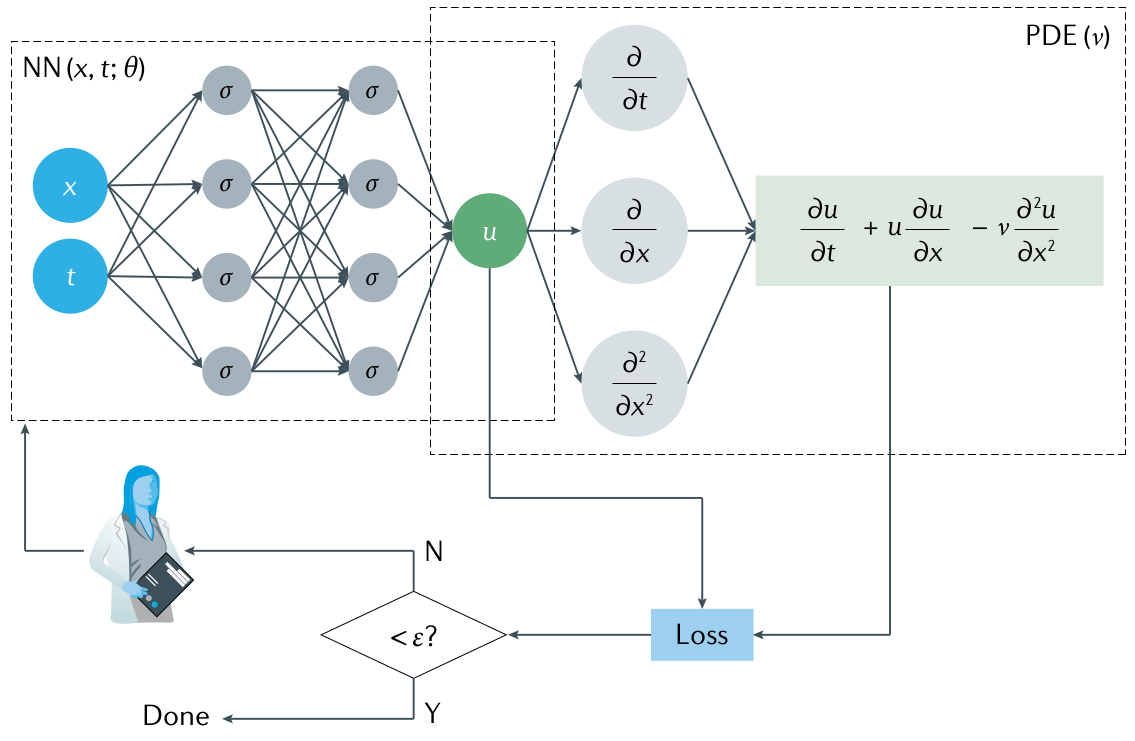
\includegraphics[width=6.25in,height=\textheight,keepaspectratio]{images/PINN_diagram.png}

}

\caption{\label{fig-pinn_graph}\textbf{El algoritmo de una PINN.}
Construya una red neuronal (NN) \(u(x, t; \theta)\) donde \(\theta\)
representa el conjunto de pesos entrenables \(w\) y sesgos \(b\), y
\(\sigma\) representa una función de activación no lineal. Especifique
los datos de medición \({x_i, t_i, u_i}\) para \(u\) y los puntos
residuales \({x_j, t_j}\) para la EDP. Especifique la pérdida
\(\mathcal{L}\) en la Ecuación~\ref{eq-loss-funct} sumando las pérdidas
ponderadas de los datos y la EDP. Entrene la NN para encontrar los
mejores parámetros \(\mathbb{\theta^*}\) minimizando la pérdida
\(\mathcal{L}\) (\citeproc{ref-karniadakis2021}{George Em Karniadakis
2021}).}

\end{figure}%

\section{Ejemplo de resolución de la ecuación de Burger 1D con
deepxde}\label{ejemplo-de-resoluciuxf3n-de-la-ecuaciuxf3n-de-burger-1d-con-deepxde}

Dada la ecuación: \[
\dfrac{\partial u}{\partial t} + u\dfrac{\partial u}{\partial x} = v\dfrac{\partial^2 u}{\partial x^2} \quad, x \in[-1,1], \ t\in[0,1]
\]

con la condición de frontera de Dirichlet y condición inicial: \[
u(-1,t) = u(1,t) = 0, \quad u(x,0)=-\sin(\pi x)
\]

\begin{Shaded}
\begin{Highlighting}[]
\ImportTok{import}\NormalTok{ deepxde }\ImportTok{as}\NormalTok{ dde}
\ImportTok{import}\NormalTok{ numpy }\ImportTok{as}\NormalTok{ np}


\KeywordTok{def}\NormalTok{ gen\_testdata():}
\NormalTok{    data }\OperatorTok{=}\NormalTok{ np.load(}\StringTok{"data/Burgers.npz"}\NormalTok{)}
\NormalTok{    t, x, exact }\OperatorTok{=}\NormalTok{ data[}\StringTok{"t"}\NormalTok{], data[}\StringTok{"x"}\NormalTok{], data[}\StringTok{"usol"}\NormalTok{].T}
\NormalTok{    xx, tt }\OperatorTok{=}\NormalTok{ np.meshgrid(x, t)}
\NormalTok{    X }\OperatorTok{=}\NormalTok{ np.vstack((np.ravel(xx), np.ravel(tt))).T}
\NormalTok{    y }\OperatorTok{=}\NormalTok{ exact.flatten()[:, }\VariableTok{None}\NormalTok{]}
    \ControlFlowTok{return}\NormalTok{ X, y}


\KeywordTok{def}\NormalTok{ pde(x, y):}
\NormalTok{    dy\_x }\OperatorTok{=}\NormalTok{ dde.grad.jacobian(y, x, i}\OperatorTok{=}\DecValTok{0}\NormalTok{, j}\OperatorTok{=}\DecValTok{0}\NormalTok{)}
\NormalTok{    dy\_t }\OperatorTok{=}\NormalTok{ dde.grad.jacobian(y, x, i}\OperatorTok{=}\DecValTok{0}\NormalTok{, j}\OperatorTok{=}\DecValTok{1}\NormalTok{)}
\NormalTok{    dy\_xx }\OperatorTok{=}\NormalTok{ dde.grad.hessian(y, x, i}\OperatorTok{=}\DecValTok{0}\NormalTok{, j}\OperatorTok{=}\DecValTok{0}\NormalTok{)}
    \ControlFlowTok{return}\NormalTok{ dy\_t }\OperatorTok{+}\NormalTok{ y }\OperatorTok{*}\NormalTok{ dy\_x }\OperatorTok{{-}} \FloatTok{0.01} \OperatorTok{/}\NormalTok{ np.pi }\OperatorTok{*}\NormalTok{ dy\_xx}


\NormalTok{geom }\OperatorTok{=}\NormalTok{ dde.geometry.Interval(}\OperatorTok{{-}}\DecValTok{1}\NormalTok{, }\DecValTok{1}\NormalTok{)}
\NormalTok{timedomain }\OperatorTok{=}\NormalTok{ dde.geometry.TimeDomain(}\DecValTok{0}\NormalTok{, }\FloatTok{0.99}\NormalTok{)}
\NormalTok{geomtime }\OperatorTok{=}\NormalTok{ dde.geometry.GeometryXTime(geom, timedomain)}

\NormalTok{bc }\OperatorTok{=}\NormalTok{ dde.icbc.DirichletBC(}
\NormalTok{    geomtime,}
    \KeywordTok{lambda}\NormalTok{ x: }\DecValTok{0}\NormalTok{,}
    \KeywordTok{lambda}\NormalTok{ \_, on\_boundary: on\_boundary)}
\NormalTok{ic }\OperatorTok{=}\NormalTok{ dde.icbc.IC(}
\NormalTok{    geomtime,}
    \KeywordTok{lambda}\NormalTok{ x: }\OperatorTok{{-}}\NormalTok{np.sin(np.pi }\OperatorTok{*}\NormalTok{ x[:, }\DecValTok{0}\NormalTok{:}\DecValTok{1}\NormalTok{]),}
    \KeywordTok{lambda}\NormalTok{ \_, on\_initial: on\_initial}
\NormalTok{)}

\NormalTok{data }\OperatorTok{=}\NormalTok{ dde.data.TimePDE(}
\NormalTok{    geomtime, pde, [bc, ic],}
\NormalTok{    num\_domain}\OperatorTok{=}\DecValTok{2540}\NormalTok{,}
\NormalTok{    num\_boundary}\OperatorTok{=}\DecValTok{80}\NormalTok{,}
\NormalTok{    num\_initial}\OperatorTok{=}\DecValTok{160}\NormalTok{,}
\NormalTok{    num\_test}\OperatorTok{=}\DecValTok{300}
\NormalTok{)}
\NormalTok{net }\OperatorTok{=}\NormalTok{ dde.nn.FNN([}\DecValTok{2}\NormalTok{] }\OperatorTok{+}\NormalTok{ [}\DecValTok{20}\NormalTok{] }\OperatorTok{*} \DecValTok{3} \OperatorTok{+}\NormalTok{ [}\DecValTok{1}\NormalTok{], }\StringTok{"tanh"}\NormalTok{, }\StringTok{"Glorot normal"}\NormalTok{)}
\NormalTok{model }\OperatorTok{=}\NormalTok{ dde.Model(data, net)}

\NormalTok{model.}\BuiltInTok{compile}\NormalTok{(}\StringTok{"adam"}\NormalTok{, lr}\OperatorTok{=}\FloatTok{1e{-}3}\NormalTok{)}
\NormalTok{losshistory, train\_state }\OperatorTok{=}\NormalTok{ model.train(iterations}\OperatorTok{=}\DecValTok{5000}\NormalTok{)}
\NormalTok{model.}\BuiltInTok{compile}\NormalTok{(}\StringTok{"L{-}BFGS"}\NormalTok{)}
\NormalTok{losshistory, train\_state }\OperatorTok{=}\NormalTok{ model.train()}
\CommentTok{\#dde.saveplot(losshistory, train\_state, issave=False, isplot=True)}
\end{Highlighting}
\end{Shaded}

\begin{Shaded}
\begin{Highlighting}[]
\ImportTok{import}\NormalTok{ matplotlib.pyplot }\ImportTok{as}\NormalTok{ plt }
\ImportTok{from}\NormalTok{ mpl\_toolkits.mplot3d }\ImportTok{import}\NormalTok{ Axes3D}

\NormalTok{X, y\_true }\OperatorTok{=}\NormalTok{ gen\_testdata()}
\NormalTok{y\_pred }\OperatorTok{=}\NormalTok{ model.predict(X)}
\NormalTok{f }\OperatorTok{=}\NormalTok{ model.predict(X, operator}\OperatorTok{=}\NormalTok{pde)}

\CommentTok{\# Extraer componentes de X}
\NormalTok{x\_coords }\OperatorTok{=}\NormalTok{ X[:, }\DecValTok{0}\NormalTok{]  }\CommentTok{\# coordenadas x (espacio)}
\NormalTok{time }\OperatorTok{=}\NormalTok{ X[:, }\DecValTok{1}\NormalTok{]      }\CommentTok{\# coordenadas t (tiempo)}

\CommentTok{\# Crear figura con dos subgráficos 3D}
\NormalTok{fig }\OperatorTok{=}\NormalTok{ plt.figure(figsize}\OperatorTok{=}\NormalTok{(}\DecValTok{12}\NormalTok{, }\DecValTok{8}\NormalTok{))}
\NormalTok{ax1 }\OperatorTok{=}\NormalTok{ fig.add\_subplot(}\DecValTok{121}\NormalTok{, projection}\OperatorTok{=}\StringTok{\textquotesingle{}3d\textquotesingle{}}\NormalTok{)}
\NormalTok{ax2 }\OperatorTok{=}\NormalTok{ fig.add\_subplot(}\DecValTok{122}\NormalTok{, projection}\OperatorTok{=}\StringTok{\textquotesingle{}3d\textquotesingle{}}\NormalTok{)}

\CommentTok{\# Calcular límites comunes para los ejes z}
\NormalTok{z\_min }\OperatorTok{=} \BuiltInTok{min}\NormalTok{(y\_true.}\BuiltInTok{min}\NormalTok{(), y\_pred.}\BuiltInTok{min}\NormalTok{())}
\NormalTok{z\_max }\OperatorTok{=} \BuiltInTok{max}\NormalTok{(y\_true.}\BuiltInTok{max}\NormalTok{(), y\_pred.}\BuiltInTok{max}\NormalTok{())}

\CommentTok{\# Gráfico 1: Valores reales}
\NormalTok{sc1 }\OperatorTok{=}\NormalTok{ ax1.scatter(x\_coords, time, y\_true, c}\OperatorTok{=}\NormalTok{y\_true,}
\NormalTok{                cmap}\OperatorTok{=}\StringTok{\textquotesingle{}viridis\textquotesingle{}}\NormalTok{, marker}\OperatorTok{=}\StringTok{\textquotesingle{}o\textquotesingle{}}\NormalTok{, vmin}\OperatorTok{=}\NormalTok{z\_min, vmax}\OperatorTok{=}\NormalTok{z\_max)}
\NormalTok{ax1.set\_xlabel(}\StringTok{\textquotesingle{}Posición (x)\textquotesingle{}}\NormalTok{)}
\NormalTok{ax1.set\_ylabel(}\StringTok{\textquotesingle{}Tiempo (t)\textquotesingle{}}\NormalTok{)}
\NormalTok{ax1.set\_zlabel(}\StringTok{\textquotesingle{}u(x,t)\textquotesingle{}}\NormalTok{)}
\NormalTok{ax1.set\_title(}\StringTok{\textquotesingle{}Valores reales de u(x,t)\textquotesingle{}}\NormalTok{)}
\NormalTok{ax1.set\_zlim([z\_min, z\_max])}

\CommentTok{\# Gráfico 2: Valores predichos}
\NormalTok{sc2 }\OperatorTok{=}\NormalTok{ ax2.scatter(x\_coords, time, y\_pred, c}\OperatorTok{=}\NormalTok{y\_pred,}
\NormalTok{                cmap}\OperatorTok{=}\StringTok{\textquotesingle{}viridis\textquotesingle{}}\NormalTok{, marker}\OperatorTok{=}\StringTok{\textquotesingle{}\^{}\textquotesingle{}}\NormalTok{, vmin}\OperatorTok{=}\NormalTok{z\_min, vmax}\OperatorTok{=}\NormalTok{z\_max)}
\NormalTok{ax2.set\_xlabel(}\StringTok{\textquotesingle{}Posición (x)\textquotesingle{}}\NormalTok{)}
\NormalTok{ax2.set\_ylabel(}\StringTok{\textquotesingle{}Tiempo (t)\textquotesingle{}}\NormalTok{)}
\NormalTok{ax2.set\_zlabel(}\StringTok{\textquotesingle{}u(x,t)\textquotesingle{}}\NormalTok{)}
\NormalTok{ax2.set\_title(}\StringTok{\textquotesingle{}Valores predichos de u(x,t)\textquotesingle{}}\NormalTok{)}
\NormalTok{ax2.set\_zlim([z\_min, z\_max])}

\NormalTok{cbar }\OperatorTok{=}\NormalTok{ fig.colorbar(sc1, ax}\OperatorTok{=}\NormalTok{(ax1,ax2),}
\NormalTok{                    shrink}\OperatorTok{=}\FloatTok{0.9}\NormalTok{, aspect}\OperatorTok{=}\DecValTok{90}\NormalTok{,}
\NormalTok{                    pad}\OperatorTok{=}\FloatTok{0.1}\NormalTok{, orientation}\OperatorTok{=}\StringTok{\textquotesingle{}horizontal\textquotesingle{}}\NormalTok{)}
\NormalTok{cbar.set\_label(}\StringTok{\textquotesingle{}Magnitud de u(x,t)\textquotesingle{}}\NormalTok{)}

\NormalTok{plt.show()}


\BuiltInTok{print}\NormalTok{(}\StringTok{"Mean residual:"}\NormalTok{, np.mean(np.absolute(f)))}
\BuiltInTok{print}\NormalTok{(}\StringTok{"L2 relative error:"}\NormalTok{, dde.metrics.l2\_relative\_error(y\_true, y\_pred))}
\end{Highlighting}
\end{Shaded}

\begin{figure}[H]

{\centering \pandocbounded{\includegraphics[keepaspectratio]{pinns_files/figure-pdf/cell-3-output-1.pdf}}

}

\caption{Resultados de la red neuronal.}

\end{figure}%

\begin{verbatim}
Mean residual: 0.0040262598
L2 relative error: 0.0027004616220110216
\end{verbatim}

\section{Comparación con Redes Neuronales
Tradicionales}\label{comparaciuxf3n-con-redes-neuronales-tradicionales}

Mientras que las redes neuronales tradicionales dependen exclusivamente
de grandes volúmenes de datos etiquetados para su entrenamiento
(\citeproc{ref-karniadakis2021}{George Em Karniadakis 2021}), las PINNs
integran el conocimiento físico como parte esencial de su arquitectura
(\citeproc{ref-blechs2021}{Blechschmidt y Ernst 2021}). Esta diferencia
clave permite a las PINNs generar soluciones físicamente consistentes
incluso con datos escasos, evitando el sobreajuste común en enfoques
puramente basados en datos. Otra ventaja significativa de las PINNs es
su naturaleza mesh-free, que contrasta con los métodos numéricos
tradicionales como FEM o FDM que requieren discretización espacial. Sin
embargo, el entrenamiento de PINNs puede ser más desafiante debido a la
necesidad de optimizar múltiples objetivos simultáneamente (ajuste a
datos y cumplimiento de leyes físicas)
(\citeproc{ref-blechs2021}{Blechschmidt y Ernst 2021};
\citeproc{ref-karniadakis2021}{George Em Karniadakis 2021}).

\chapter{DeepONet}\label{deeponet}

\textbf{DeepONet} (Deep Operator Network) es una arquitectura de red
neuronal profunda diseñada para aprender operadores no lineales que
mapean funciones de entrada a funciones de salida. A diferencia de las
redes convencionales que aprenden funciones escalares, DeepONet se
enfoca en representar operadores completos, como soluciones de
ecuaciones diferenciales, a partir de datos observados o simulaciones
numéricas (\citeproc{ref-lu2021deeponet}{Lu, Jin, et~al. 2021}).

\section{Arquitectura}\label{arquitectura}

La arquitectura de DeepONet está compuesta por dos redes principales: la
red de \emph{branch} y la red de \emph{trunk}. La red \emph{branch}
procesa las evaluaciones discretas de la función de entrada (por
ejemplo, condiciones iniciales o de frontera), mientras que la red
\emph{trunk} recibe como entrada los puntos del dominio donde se desea
evaluar la función de salida. La salida final se obtiene mediante el
producto punto de los vectores generados por ambas redes, lo que permite
representar operadores complejos con alta generalización a nuevos datos
(\citeproc{ref-lu2021deeponet}{Lu, Jin, et~al. 2021}).

\begin{figure}

\centering{

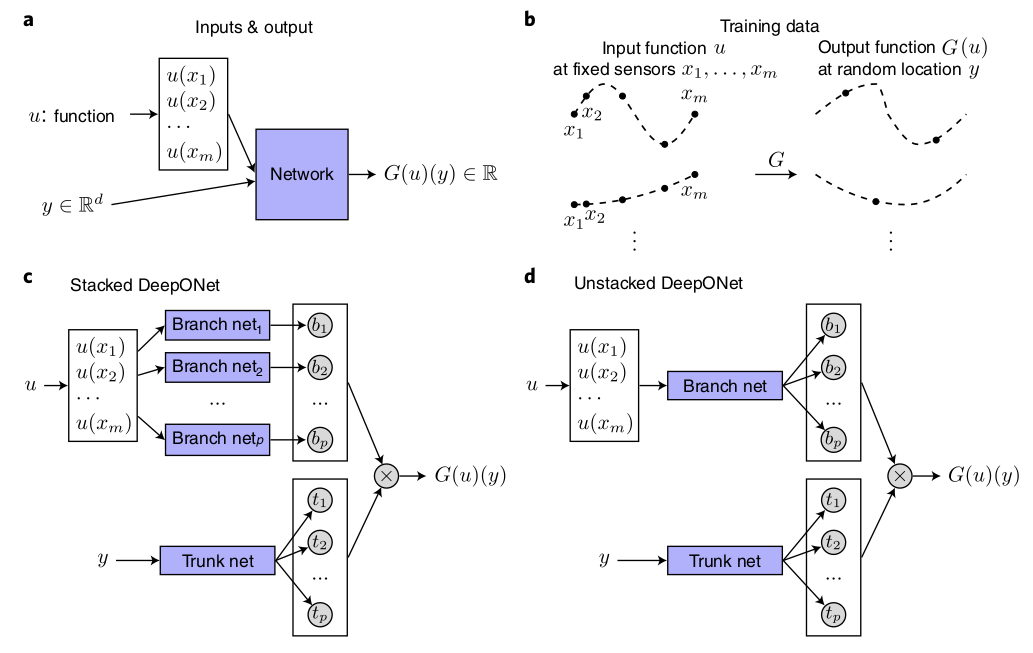
\includegraphics[width=6.25in,height=\textheight,keepaspectratio]{images/deeponet_architecture.png}

}

\caption{\label{fig-deeponet-arch}\textbf{Ilustraciones del
planteamiento del problema y arquitectura DeepONet que conducen a una
buena generalización. a)} Para que la red aprenda un operador
\(G : u \rightarrow G(u)\) se necesitan dos entradas
\([u(x_1), u(x_2), ..., u(x_m)]\) e \(y\). \textbf{b)} Ilustración de
los datos de entrenamiento. Para cada función de entrada \(u\), se
requiere el mismo número de evaluaciones en los mismos sensores
dispersos \(x_1, x_2, ..., x_m\). Sin embargo, no se impone ninguna
restricción sobre el número ni las ubicaciones para la evaluación de las
funciones de salida. \textbf{c)} La DeepONet \emph{stacked} se inspira
en el \textbf{Teorema de aproximación universal para operadores} y
consta de una red \emph{Trunk} y \(p\) redes \emph{Branch} apiladas. La
red cuya construcción se inspira en el mismo teorema es una DeepONet
\emph{stacked} formada al elegir la red \emph{Trunk} como una red de una
capa de ancho \(p\) y cada red \emph{Branch} como una red de una capa
oculta de ancho \(n\). \textbf{d)} La red DeepONet \emph{unstacked} se
inspira en el \textbf{Teorema general de aproximación universal para
operadores} y consta de una red \emph{Trunk} y una red \emph{Branch}.
Una red DeepONet \emph{unstacked} puede considerarse como una red
DeepONet \emph{stacked}, en la que todas las redes \emph{Branch}
comparten el mismo conjunto de parámetros
(\citeproc{ref-lu2021deeponet}{Lu, Jin, et~al. 2021}).}

\end{figure}%

\section{Ejemplo de resolución de un operador usando
DeepONet}\label{ejemplo-de-resoluciuxf3n-de-un-operador-usando-deeponet}

Se resolverá el operador \[
G: f\rightarrow u
\]

para el problema unidimensional de Poisson: \[
u''(x) = f(x), \quad x\in[0,1]
\]

con la condición de frontera de Dirichlet \[
u(0)=u(1)=0
\]

el término \(f\) representa a una función continua arbitraria.

\begin{Shaded}
\begin{Highlighting}[]
\ImportTok{import}\NormalTok{ deepxde }\ImportTok{as}\NormalTok{ dde}
\ImportTok{import}\NormalTok{ matplotlib.pyplot }\ImportTok{as}\NormalTok{ plt}
\ImportTok{import}\NormalTok{ numpy }\ImportTok{as}\NormalTok{ np}


\CommentTok{\# Poisson equation: {-}u\_xx = f}
\KeywordTok{def}\NormalTok{ equation(x, y, f):}
\NormalTok{    dy\_xx }\OperatorTok{=}\NormalTok{ dde.grad.hessian(y, x)}
    \ControlFlowTok{return} \OperatorTok{{-}}\NormalTok{dy\_xx }\OperatorTok{{-}}\NormalTok{ f}

\CommentTok{\# Domain is interval [0, 1]}
\NormalTok{geom }\OperatorTok{=}\NormalTok{ dde.geometry.Interval(}\DecValTok{0}\NormalTok{, }\DecValTok{1}\NormalTok{)}

\CommentTok{\# Zero Dirichlet BC}
\KeywordTok{def}\NormalTok{ u\_boundary(\_):}
    \ControlFlowTok{return} \DecValTok{0}

\KeywordTok{def}\NormalTok{ boundary(\_, on\_boundary):}
    \ControlFlowTok{return}\NormalTok{ on\_boundary}

\NormalTok{bc }\OperatorTok{=}\NormalTok{ dde.icbc.DirichletBC(geom, u\_boundary, boundary)}

\CommentTok{\# Define PDE}
\NormalTok{pde }\OperatorTok{=}\NormalTok{ dde.data.PDE(geom, equation, bc, num\_domain}\OperatorTok{=}\DecValTok{100}\NormalTok{, num\_boundary}\OperatorTok{=}\DecValTok{2}\NormalTok{)}

\CommentTok{\# Function space for f(x) are polynomials}
\NormalTok{degree }\OperatorTok{=} \DecValTok{3}
\NormalTok{space }\OperatorTok{=}\NormalTok{ dde.data.PowerSeries(N}\OperatorTok{=}\NormalTok{degree }\OperatorTok{+} \DecValTok{1}\NormalTok{)}

\CommentTok{\# Choose evaluation points}
\NormalTok{num\_eval\_points }\OperatorTok{=} \DecValTok{10}
\NormalTok{evaluation\_points }\OperatorTok{=}\NormalTok{ geom.uniform\_points(num\_eval\_points, boundary}\OperatorTok{=}\VariableTok{True}\NormalTok{)}

\CommentTok{\# Define PDE operator}
\NormalTok{pde\_op }\OperatorTok{=}\NormalTok{ dde.data.PDEOperatorCartesianProd(}
\NormalTok{    pde,}
\NormalTok{    space,}
\NormalTok{    evaluation\_points,}
\NormalTok{    num\_function}\OperatorTok{=}\DecValTok{100}\NormalTok{,}
\NormalTok{    num\_test}\OperatorTok{=}\DecValTok{20}
\NormalTok{)}

\CommentTok{\# Setup DeepONet}
\NormalTok{dim\_x }\OperatorTok{=} \DecValTok{1}
\NormalTok{p }\OperatorTok{=} \DecValTok{32}
\NormalTok{net }\OperatorTok{=}\NormalTok{ dde.nn.DeepONetCartesianProd(}
\NormalTok{    [num\_eval\_points, }\DecValTok{32}\NormalTok{, p],}
\NormalTok{    [dim\_x, }\DecValTok{32}\NormalTok{, p],}
\NormalTok{    activation}\OperatorTok{=}\StringTok{"tanh"}\NormalTok{,}
\NormalTok{    kernel\_initializer}\OperatorTok{=}\StringTok{"Glorot normal"}\NormalTok{,}
\NormalTok{)}

\CommentTok{\# Define and train model}
\NormalTok{model }\OperatorTok{=}\NormalTok{ dde.Model(pde\_op, net)}
\NormalTok{dde.optimizers.set\_LBFGS\_options(maxiter}\OperatorTok{=}\DecValTok{1000}\NormalTok{)}
\NormalTok{model.}\BuiltInTok{compile}\NormalTok{(}\StringTok{"L{-}BFGS"}\NormalTok{)}
\NormalTok{model.train()}

\CommentTok{\# Plot realisations of f(x)}
\NormalTok{n }\OperatorTok{=} \DecValTok{3}
\NormalTok{features }\OperatorTok{=}\NormalTok{ space.random(n)}
\NormalTok{fx }\OperatorTok{=}\NormalTok{ space.eval\_batch(features, evaluation\_points)}

\NormalTok{x }\OperatorTok{=}\NormalTok{ geom.uniform\_points(}\DecValTok{100}\NormalTok{, boundary}\OperatorTok{=}\VariableTok{True}\NormalTok{)}
\NormalTok{y }\OperatorTok{=}\NormalTok{ model.predict((fx, x))}
\end{Highlighting}
\end{Shaded}

\begin{Shaded}
\begin{Highlighting}[]
\CommentTok{\# Setup figure}
\NormalTok{fig }\OperatorTok{=}\NormalTok{ plt.figure(figsize}\OperatorTok{=}\NormalTok{(}\DecValTok{7}\NormalTok{, }\DecValTok{8}\NormalTok{))}
\NormalTok{plt.subplot(}\DecValTok{2}\NormalTok{, }\DecValTok{1}\NormalTok{, }\DecValTok{1}\NormalTok{)}
\NormalTok{plt.title(}\StringTok{"Ecuación de Poisson: término f(x) y solución u(x)"}\NormalTok{)}
\NormalTok{plt.ylabel(}\StringTok{"f(x)"}\NormalTok{)}
\NormalTok{z }\OperatorTok{=}\NormalTok{ np.zeros\_like(x)}
\NormalTok{plt.plot(x, z, }\StringTok{"k{-}"}\NormalTok{, alpha}\OperatorTok{=}\FloatTok{0.1}\NormalTok{)}

\CommentTok{\# Plot source term f(x)}
\ControlFlowTok{for}\NormalTok{ i }\KeywordTok{in} \BuiltInTok{range}\NormalTok{(n):}
\NormalTok{    plt.plot(evaluation\_points, fx[i], }\StringTok{"{-}{-}"}\NormalTok{)}

\CommentTok{\# Plot solution u(x)}
\NormalTok{plt.subplot(}\DecValTok{2}\NormalTok{, }\DecValTok{1}\NormalTok{, }\DecValTok{2}\NormalTok{)}
\NormalTok{plt.ylabel(}\StringTok{"u(x)"}\NormalTok{)}
\NormalTok{plt.plot(x, z, }\StringTok{"k{-}"}\NormalTok{, alpha}\OperatorTok{=}\FloatTok{0.1}\NormalTok{)}
\ControlFlowTok{for}\NormalTok{ i }\KeywordTok{in} \BuiltInTok{range}\NormalTok{(n):}
\NormalTok{    plt.plot(x, y[i], }\StringTok{"{-}"}\NormalTok{)}
\NormalTok{plt.xlabel(}\StringTok{"x"}\NormalTok{)}

\NormalTok{plt.show()}
\end{Highlighting}
\end{Shaded}

\begin{figure}[H]

{\centering \pandocbounded{\includegraphics[keepaspectratio]{deeponet_files/figure-pdf/cell-3-output-1.pdf}}

}

\caption{Resultados de la red DeepONet.}

\end{figure}%

\section{Comparación con una PINN}\label{comparaciuxf3n-con-una-pinn}

En contraste con una red PINN convencional (Physics-Informed Neural
Network), que resuelve una instancia específica de una ecuación
diferencial para un conjunto dado de condiciones, DeepONet aprende el
operador general que resuelve muchas instancias a la vez. Mientras que
una PINN debe ser reentrenada para cada nuevo problema, DeepONet, una
vez entrenado, puede predecir soluciones rápidamente para múltiples
condiciones nuevas. Esto lo hace especialmente eficiente en aplicaciones
donde se requiere realizar inferencias repetidas, como en control o
diseño inverso (\citeproc{ref-kumar2024deeponet}{Kumar et~al. 2024}).

\part{Ecuación del Bio-Calor}

La ecuación del bio-calor, formulada por Pennes
(\citeproc{ref-pennes1948}{1948}), surgió de su estudio pionero
\emph{``Analysis of Tissue and Arterial Blood Temperatures in the
Resting Human Forearm''}. Publicado en el \emph{Journal of Applied
Physiology}, este trabajo fue el primero en cuantificar la interacción
entre la temperatura arterial y tisular en humanos. Pennes combinó
principios termodinámicos con mediciones experimentales en el antebrazo,
estableciendo un modelo matemático que relacionaba el flujo sanguíneo,
la producción metabólica de calor y la conducción térmica en tejidos.

\section*{Experimento}\label{experimento}
\addcontentsline{toc}{section}{Experimento}

\markright{Experimento}

Durante su estudio, Pennes diseñó un experimento riguroso para medir la
temperatura interna del antebrazo humano. Utilizó termopares tipo ``Y''
insertados transversalmente en la musculatura del antebrazo mediante una
aguja estéril, como se ilustra en la Figura~\ref{fig-pennes_art}. Esta
configuración permitía capturar un perfil térmico a lo largo del eje
transversal, minimizando interferencias derivadas del contacto externo o
la conducción axial no deseada.

La técnica experimental buscó máxima precisión geométrica y térmica: los
termopares eran fijados con tensión controlada mediante un sistema
mecánico que aseguraba trayectorias rectas y repetibles dentro del
tejido. La inserción se realizaba con anestesia tópica mínima y bajo
condiciones ambientales estables, lo cual garantizaba que los gradientes
de temperatura registrados fueran atribuibles principalmente al
metabolismo local y al efecto del flujo sanguíneo arterial.

\begin{figure}

\centering{

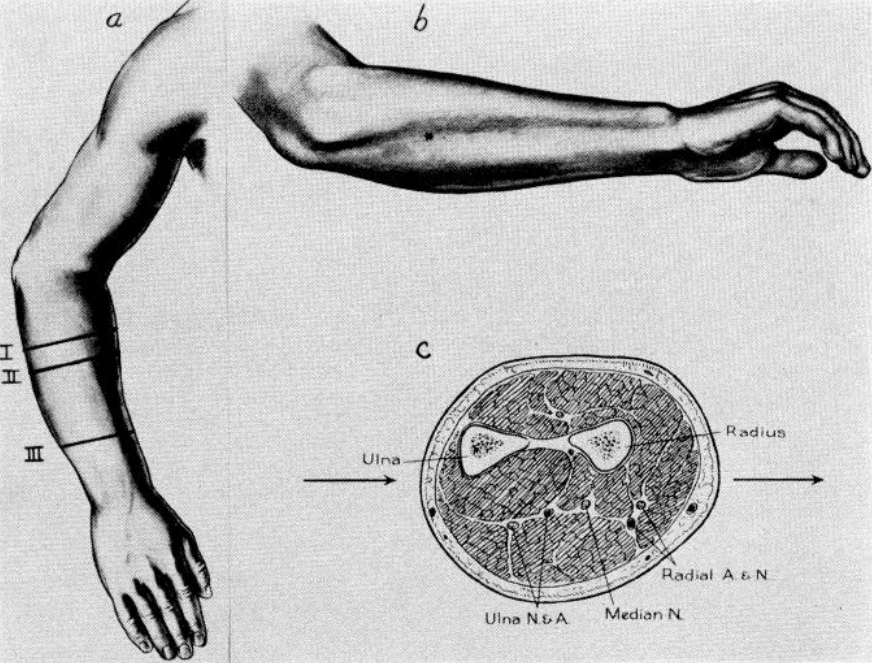
\includegraphics[width=5.20833in,height=\textheight,keepaspectratio]{images/pennes_art.png}

}

\caption{\label{fig-pennes_art}\textbf{a)} Posición del brazo derecho
(vista superior). La linea horizontal II indica el nivel de la figura
c). \textbf{b)} Posición del brazo derecho (vista lateral).
\textbf{c)}Sección transversal anatómica del antebrazo en el nivel II
(\citeproc{ref-pennes1948}{Pennes 1948}).}

\end{figure}%

\section*{Trascendencia}\label{trascendencia}
\addcontentsline{toc}{section}{Trascendencia}

\markright{Trascendencia}

El modelo de Pennes simplificó la complejidad biológica al asumir un
flujo sanguíneo uniforme y una transferencia de calor proporcional a la
diferencia entre la temperatura arterial y la tisular. Aunque
posteriores investigaciones refinaron sus supuestos, su ecuación sigue
siendo un referente en bioingeniería térmica. Su trabajo no solo sentó
las bases para aplicaciones clínicas, como la hipertermia oncológica,
sino que también inspiró avances en el estudio de la termorregulación
humana y el diseño de dispositivos médicos.

\chapter{Forma de la ecuación}\label{forma-de-la-ecuaciuxf3n}

La ecuación diferencial de bio-calor de Pennes
(\citeproc{ref-pennes1948}{1948}) modela la transferencia de calor en
tejidos biológicos, integrando efectos de conducción, perfusión
sanguínea y metabolismo. Su forma general es:

\begin{equation}\phantomsection\label{eq-PBHE_completa}{
\rho c \frac{\partial T}{\partial t} = k_{\text{eff}} \frac{\partial^{2} T}{\partial x^{2}} - \rho_b c_b \omega_b (T - T_a) + Q, \quad x \in \Omega, \, t \in [0, t_f]
}\end{equation}

\begin{longtable}[]{@{}lll@{}}
\caption{Tabla de nomenclaturas de la
Ecuación~\ref{eq-PBHE_completa}.}\label{tbl-nomenclatura-PBHE_completa}\tabularnewline
\toprule\noalign{}
Símbolo & Descripción & Unidades \\
\midrule\noalign{}
\endfirsthead
\toprule\noalign{}
Símbolo & Descripción & Unidades \\
\midrule\noalign{}
\endhead
\bottomrule\noalign{}
\endlastfoot
\(T\) & Temperatura del tejido & °C \\
\(\rho\) & Densidad del tejido & \(\frac{kg}{m^3}\) \\
\(c\) & Calor específico del tejido & \(\frac{J}{kg °C}\) \\
\(k_{\text{eff}}\) & Conductividad térmica & \(\frac{W}{m °C}\) \\
\(\rho_b\) & Densidad de la sangre & \(\frac{kg}{m^3}\) \\
\(c_b\) & Calor específico de la sangre & \(\frac{J}{kg °C}\) \\
\(\omega_b\) & Tasa de perfusión sanguínea & \(1/s\) \\
\(T_a\) & Temperatura arterial & °C \\
\(Q = q_m + q_p\) & Fuente de calor & \(\frac{W}{m^3}\) \\
\(q_m\) & Metabolismo & \(\frac{W}{m^3}\) \\
\(q_p\) & Externa & \(\frac{W}{m^3}\) \\
\end{longtable}

\section{Versión reducida
(adimensionalizada)}\label{versiuxf3n-reducida-adimensionalizada}

Mediante escalamiento: \begin{equation*}
T' = T - T_a \qquad \theta = \dfrac{T'}{T_M - T_a} \qquad X = \dfrac{x}{L_0} \qquad \tau = \dfrac{t}{t_f}
\end{equation*}

\begin{longtable}[]{@{}lll@{}}
\caption{Tabla de nomenclatura de las relaciones para
escalamiento.}\label{tbl-}\tabularnewline
\toprule\noalign{}
Símbolo & Descripción & Unidades \\
\midrule\noalign{}
\endfirsthead
\toprule\noalign{}
Símbolo & Descripción & Unidades \\
\midrule\noalign{}
\endhead
\bottomrule\noalign{}
\endlastfoot
\(L_0\) & Longitud característica del dominio & \(m\) \\
\(t_f\) & Tiempo final de simulación & \(s\) \\
\end{longtable}

la Ecuación~\ref{eq-PBHE_completa} se convierte en:

\begin{equation}\phantomsection\label{eq-PBHE-reduced}{
\partial_{\tau} \theta = a_1 \partial_{XX} \theta - a_2 W \theta + a_3
}\end{equation}

\textbf{Parámetros adimensionales}:\\
- \(a_1 = \frac{t_f}{\alpha L_0^2}\) (difusividad térmica
\(\alpha = \frac{k_{\text{eff}}}{\rho c}\)).\\
- \(a_2 = \frac{t_f c_b}{\rho c}\).\\
- \(a_3 = \frac{t_f Q}{\rho c (T_M - T_a)}\).\\
- \(W = \rho_b \omega_b\): Tasa volumétrica de perfusión (kg/m³·s).

\section{Condiciones de uso
adecuadas}\label{condiciones-de-uso-adecuadas}

\begin{enumerate}
\def\labelenumi{\arabic{enumi}.}
\tightlist
\item
  \textbf{Tejidos homogéneos}: Aproximación válida para regiones con
  propiedades térmicas uniformes.\\
\item
  \textbf{Perfusión sanguínea constante}: Supone flujo sanguíneo estable
  en el dominio.\\
\item
  \textbf{Aplicaciones clínicas}: Hipertermia, crioterapia y modelado
  térmico en terapias oncológicas.
\end{enumerate}

\chapter{Modelado del Bio-Calor en
Hipertermia}\label{modelado-del-bio-calor-en-hipertermia}

La ecuación del bio-calor, formulada por Pennes
(\citeproc{ref-pennes1948}{1948}), permite modelar la distribución de
temperatura en tejidos biológicos considerando el flujo sanguíneo, la
conductividad térmica y fuentes internas o externas de calor. Su
modelación es fundamental en la física médica para predecir el
comportamiento térmico durante tratamientos como la hipertermia. Además,
constituye una herramienta poderosa en el desarrollo de simulaciones
computacionales aplicadas al diseño y control de terapias térmicas en
tejidos vivos.

\section{Aplicaciones recientes de la ecuación del
bio-calor}\label{aplicaciones-recientes-de-la-ecuaciuxf3n-del-bio-calor}

Quintero et~al. (\citeproc{ref-quintero2017}{2017}) desarrollan un
modelo basado en ecuaciones diferenciales parciales que integra la
ecuación del bio-calor y la ley de Arrhenius para estimar el daño
térmico en tratamientos de hipertermia superficial. Utilizan el método
de líneas para resolver el sistema y plantean un problema de
optimización que busca maximizar el daño al tejido tumoral minimizando
el daño colateral. Su trabajo demuestra cómo la modelación matemática
puede guiar estrategias terapéuticas más seguras y eficaces.

Dutta y Rangarajan (\citeproc{ref-dutta2018}{2018}) presentan una
solución analítica cerrada en dos dimensiones para la ecuación del
bio-calor, considerando modelos de conducción tanto de tipo Fourier como
no-Fourier. Mediante el uso de la transformada de Laplace, analizan la
influencia de parámetros fisiológicos como la perfusión sanguínea y el
tiempo de relajación térmica sobre la evolución de la temperatura. Su
investigación aporta una base teórica sólida para comprender la
propagación térmica en tejidos vivos durante la hipertermia terapéutica.

Yang et~al. (\citeproc{ref-yang2014}{2014}) propone una estrategia
numérica para resolver problemas inversos de conducción térmica en
tejidos biológicos multicapa, utilizando un enfoque en diferencias
finitas y el concepto de tiempo futuro. El estudio se enfoca en predecir
las condiciones de frontera necesarias para generar distribuciones de
temperatura deseadas. La implementación de este método permite estimar
parámetros relevantes en tiempo real, lo cual resulta esencial para el
control térmico preciso en procedimientos médicos no invasivos como la
hipertermia localizada.

\part{Estudio de caso}

\section*{Hipertermia como opción terapéutica complementaria en el
manejo de
cáncer}\label{hipertermia-como-opciuxf3n-terapuxe9utica-complementaria-en-el-manejo-de-cuxe1ncer}
\addcontentsline{toc}{section}{Hipertermia como opción terapéutica
complementaria en el manejo de cáncer}

\markright{Hipertermia como opción terapéutica complementaria en el
manejo de cáncer}

La Organización Mundial de la Salud (\citeproc{ref-omscancer}{2022}) en
su página web define Cáncer como:

\emph{«Cáncer» es un término genérico utilizado para designar un amplio
grupo de enfermedades que pueden afectar a cualquier parte del
organismo; también se habla de «tumores malignos» o «neoplasias
malignas». Una característica definitoria del cáncer es la
multiplicación rápida de células anormales que se extienden más allá de
sus límites habituales y pueden invadir partes adyacentes del cuerpo o
propagarse a otros órganos, en un proceso que se denomina «metástasis».
La extensión de las metástasis es la principal causa de muerte por la
enfermedad.}

Por su parte Instituto Nacional del Cáncer
(\citeproc{ref-nci2021}{2021}) aporta lo siguiente:

\emph{Es posible que el cáncer comience en cualquier parte del cuerpo
humano, formado por billones de células. En condiciones normales, las
células humanas se forman y se multiplican (mediante un proceso que se
llama división celular) para formar células nuevas a medida que el
cuerpo las necesita. Cuando las células envejecen o se dañan, mueren y
las células nuevas las reemplazan.} \emph{A veces el proceso no sigue
este orden y las células anormales o células dañadas se forman y se
multiplican cuando no deberían. Estas células tal vez formen tumores,
que son bultos de tejido. Los tumores son cancerosos (malignos) o no
cancerosos (benignos).}

\begin{figure}

\centering{

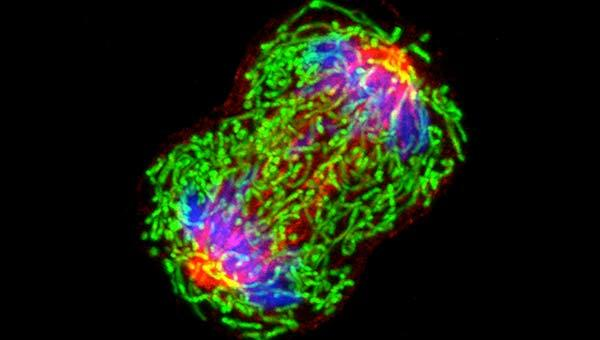
\includegraphics[width=5.20833in,height=\textheight,keepaspectratio]{images/dividing-breast-cancer-cell.jpg}

}

\caption{\label{fig-breast-cancer}Una célula de cáncer de seno que se
multiplica (\citeproc{ref-nci2021}{Instituto Nacional del Cáncer
2021}).}

\end{figure}%

Ésta enfermedad es la principal causa de muerte a nivel mundial, solo en
2020 arrebató casi 10 millones de vidas y según datos de Organización
Mundial de la Salud (\citeproc{ref-omscancer}{2022}) los cánceres más
comunes en 2020 fueron:

\begin{itemize}
\tightlist
\item
  De mama (2.26 millones de casos)
\item
  De pulmón (2.21 millones de casos)
\item
  De colon (1.93 millones de casos)
\item
  De próstata (1.41 millones de casos)
\item
  De piel (distinto del melanoma) (1.20 millones de casos)
\item
  Gástrico (1.09 millones de casos)
\end{itemize}

Es ante este panorama que distintos tratamientos surgen con el objetivo
de erradicar la enfermedad siempre que se tenga una detección oportuna.
Uno de dichos tratamientos es la hipertermia, según en el National
Cancer Institute (\citeproc{ref-hyperthermia}{2021}) es un método que
consiste en calentar el tejido corporal hasta los 39-45 °C para ayudar a
erradicar células cancerígenas con pequeñas o nulas lesiones en el
tejido sano. La hipertermia también es llamada terapia térmica o
termoterapia.

Uno de los principales retos de este tratamiento es la creación de un
modelo óptimo que se adecue al comportamiento de la transferencia de
calor que se hace a los tejidos con el fin de dañar únicamente el área
en el que se encuentran las células cancerígenas, es por ello que los
modelos de inteligencia artificial y más precisamente las PINN's
Capítulo~\ref{sec-pinns} surgen como posible solución a este reto.

El presente estudio utilizó como punto de partida el trabajo realizado
por Alessio Borgi (\citeproc{ref-medical_rep}{2023}) para modelar el
calentamiento del tejido corporal usando la ecuación del Bio-Calor en
dos dimensiones.

\chapter{Metodología}\label{metodologuxeda}

En esta sección se describe el enfoque metodológico utilizado para
evaluar la efectividad de una PINN utilizando una arquitectura DeepONet
con el objetivo de resolver la ecuacion del Bio-Calor. El proceso
metodológico se divide en las siguientes etapas:

\section{Aportaciones del modelo}\label{aportaciones-del-modelo}

Ya que se parte del trabajo de Alessio Borgi
(\citeproc{ref-medical_rep}{2023}), se examinó que dos de los puntos a
mejorar de la red neuronal que plantearon son:

\begin{enumerate}
\def\labelenumi{\arabic{enumi}.}
\tightlist
\item
  Desarrollar nuevas arquitecturas para la red neuronal y explorar
  nuevas configuraciones.
\item
  Combinar las fortalezas de los algoritmos de optimización Adam y
  L-BFGS para mejorar la velocidad de convergencia y la precisión.
\end{enumerate}

Teniendo los anteriores puntos en cuenta, se procedió a abordarlos e
implementarlos dentro del diseño del modelo.

\section{Diseño del modelo}\label{diseuxf1o-del-modelo}

El lenguaje seleccionado fué Python, a su vez el código se basa
enteramente en la librería Deepxde creada por Lu, Meng, et~al.
(\citeproc{ref-deepxde}{2021}) la cual está directamente enfocada a
resolver ecuaciones diferenciales, se usó además como backend
\emph{tensorflow\_compat\_v1} siendo su elección debida únicamente a la
familiarización previa que se tenía con ella. Finalmente el entorno
donde se programó y optimizó el código fué en \emph{Google Colab} ya que
la potencia de cómputo ofrecida por la plataforma era necesaria para
ejecutar el modelo.

\section{Implementación del modelo}\label{implementaciuxf3n-del-modelo}

La implementación del modelo se llevó a cabo en dos etapas clave:
\textbf{(1) el desarrollo del código base para resolver la ecuación del
Bio-Calor mediante DeepXDE}, y \textbf{(2) la optimización sistemática
de los hiperparámetros}. Para esta última, se siguieron las
recomendaciones del estudio de Alessio Borgi
(\citeproc{ref-medical_rep}{2023}), adaptadas a las particularidades del
problema. Se ajustaron parámetros críticos como el número de épocas de
entrenamiento (\emph{iterations}), el ratio de aprendizaje
(\emph{learning rate}) así como un decaimiento en el mismo dependiente
de la iteración actual (\emph{decay}), la función de activación
(\emph{elu}) y el esquema de inicialización de pesos (\emph{Glorot
normal}). Estos ajustes se realizaron mediante un proceso iterativo que
buscaba minimizar la función de pérdida mientras se mantenía un tiempo
de entrenamiento computacionalmente viable.

\section{Evaluación del modelo}\label{evaluaciuxf3n-del-modelo}

Para validar el desempeño del modelo propuesto, se realizó una
evaluación exhaustiva utilizando un \emph{conjunto de datos
independiente}, el cual no fue empleado durante las fases de
entrenamiento o ajuste de hiperparámetros. Este enfoque garantiza una
medición objetiva de la capacidad de generalización del modelo ante
datos no vistos.

Las predicciones generadas por el modelo fueron analizadas mediante
visualizaciones espaciotemporales, las cuales permiten comparar
cualitativamente el comportamiento de las soluciones pronosticadas
frente a los rangos físicos y temporales definidos en el problema. En
particular, se generaron gráficas de superficies 3D que muestran la
evolución de las variables de interés a lo largo del dominio espacial y
temporal bajo estudio. Adicionalmente, se incluyeron representaciones de
cortes transversales y series temporales en puntos estratégicos para
facilitar la interpretación de los resultados.

Cabe destacar que este análisis preliminar se centró en examinar la
coherencia física y la estabilidad numérica de las predicciones. Para la
evaluación cuantitativa del modelo, se implementó una comparación
directa con las soluciones obtenidas mediante el método numérico de
\textbf{Crank-Nicolson}, resuelto en \emph{Julia} utilizando la librería
\emph{DifferentialEquations.jl}.

\section{Comparación de resultados}\label{comparaciuxf3n-de-resultados}

Para evaluar el desempeño predictivo del modelo propuesto, se realizaron
dos tipos de comparaciones:

\begin{enumerate}
\def\labelenumi{\arabic{enumi}.}
\tightlist
\item
  Una evaluación cualitativa basada en visualizaciones.
\item
  Un análisis cuantitativo mediante métricas de error estandarizadas.
\end{enumerate}

En primer lugar, se llevó a cabo una comparación visual con los
resultados reportados en el trabajo de Alessio Borgi
(\citeproc{ref-medical_rep}{2023}), dado que dicho estudio no incluye
datos numéricos tabulados, sino únicamente representaciones gráficas de
las soluciones. Esta comparación permitió identificar coincidencias y
discrepancias en el comportamiento espaciotemporal de las variables de
interés, destacando las fortalezas del modelo propuesto en términos de
estabilidad numérica.

En segundo lugar, para una evaluación cuantitativa rigurosa, se
compararon las predicciones del modelo con soluciones de referencia
generadas mediante el método de Crank-Nicolson, implementado en Julia
utilizando la librería DifferentialEquations.jl. La comparación se
realizó sobre una malla uniforme de 26×26 puntos en el cuadrado de
\([0,1]\times[0,1]\), calculando para cada instante de tiempo relevante
las siguientes métricas:

\begin{itemize}
\tightlist
\item
  Error Absoluto Medio (MAE).
\item
  Error Absoluto Máximo (MaxAE).
\item
  Error L2 (norma euclidiana).
\end{itemize}

Estos criterios permitieron cuantificar no solo la precisión global del
modelo, sino también sus desviaciones locales más significativas,
particularmente en regiones con alta variabilidad espacial. Los
resultados detallados de este análisis, junto con una discusión sobre la
eficiencia computacional relativa entre ambos métodos, se presentan en
la Tabla~\ref{tbl-errores}.

\section{Análisis y conclusión}\label{anuxe1lisis-y-conclusiuxf3n}

Finalmente, se realizó un análisis detallado de los resultados obtenidos
para extraer conclusiones significativas. Se proporcionaron
recomendaciones basadas en los hallazgos del estudio, lo que permitió
establecer un marco para interpretaciones analíticas profundas y
recomendaciones bien fundamentadas en la sección de conclusiones del
estudio.

Este enfoque metodológico proporcionó una base sólida para los
resultados obtenidos, asegurando la integridad y la calidad del análisis
realizado en el estudio.

\chapter{Predicciones del método
numérico}\label{predicciones-del-muxe9todo-numuxe9rico}

Para validar los resultados del modelo propuesto, se implementó el
método de Crank-Nicolson en Julia utilizando la librería
\emph{DifferentialEquations.jl}. El método se resolvió sobre una malla
refinada de 51×51 puntos para garantizar alta precisión en la solución
numérica, calculando las predicciones en los tiempos clave: t = {[}0.0,
0.25, 0.50, 0.75, 1.0{]}. En la Figura~\ref{fig-met-crank-nick} se
muestran las cinco gráficas generadas, las cuales ilustran la evolución
temporal de la solución en el dominio de estudio.

\begin{Shaded}
\begin{Highlighting}[]
\ImportTok{using} \BuiltInTok{DifferentialEquations}\NormalTok{, }\BuiltInTok{LinearAlgebra}
\ImportTok{using} \BuiltInTok{DataFrames}\NormalTok{, }\BuiltInTok{CSV}

\CommentTok{\# {-}{-}{-} PARÁMETROS FÍSICOS Y DIMENSIONALES {-}{-}{-}{-}{-}{-}{-}{-}{-}{-}{-}{-}{-}{-}{-}{-}{-}{-}{-}{-}{-}{-}{-}{-}{-}{-}{-}{-}{-}{-}{-}{-}{-}{-}}
\NormalTok{p, c  }\OperatorTok{=} \FloatTok{1050.0}\NormalTok{, }\FloatTok{3639.0}                       \CommentTok{\# densidad, calor específico }
\NormalTok{k\_eff }\OperatorTok{=} \FloatTok{5.0}                                  \CommentTok{\# conductividad}
\NormalTok{t\_f   }\OperatorTok{=} \FloatTok{1800.0}                               \CommentTok{\# tiempo final }
\NormalTok{L     }\OperatorTok{=} \FloatTok{0.05}                                 \CommentTok{\# longitud del dominio}
\NormalTok{c\_b   }\OperatorTok{=} \FloatTok{3825.0}                               \CommentTok{\# coef. perfusión}
\NormalTok{Q     }\OperatorTok{=} \FloatTok{0.0}                                  \CommentTok{\# fuente térmica}
\NormalTok{T\_M, T\_a }\OperatorTok{=} \FloatTok{45.0}\NormalTok{, }\FloatTok{37.0}                        \CommentTok{\# temp máxima, temp ambiente}

\CommentTok{\# {-}{-}{-} COEFICIENTES ADIMENSIONALES {-}{-}{-}{-}{-}{-}{-}{-}{-}{-}{-}{-}{-}{-}{-}{-}{-}{-}{-}{-}{-}{-}{-}{-}{-}{-}{-}{-}{-}{-}{-}{-}{-}{-}{-}{-}{-}{-}{-}{-}{-}}
\NormalTok{α }\OperatorTok{=}\NormalTok{ p }\OperatorTok{*}\NormalTok{ c }\OperatorTok{/}\NormalTok{ k\_eff}
\NormalTok{a₁ }\OperatorTok{=}\NormalTok{ t\_f }\OperatorTok{/}\NormalTok{ (α }\OperatorTok{*}\NormalTok{ L}\OperatorTok{\^{}}\FloatTok{2}\NormalTok{)}
\NormalTok{a₂ }\OperatorTok{=}\NormalTok{ t\_f }\OperatorTok{*}\NormalTok{ c\_b }\OperatorTok{/}\NormalTok{ (p }\OperatorTok{*}\NormalTok{ c)}
\NormalTok{a₃ }\OperatorTok{=}\NormalTok{ (t\_f }\OperatorTok{*}\NormalTok{ Q) }\OperatorTok{/}\NormalTok{ (p }\OperatorTok{*}\NormalTok{ c }\OperatorTok{*}\NormalTok{ (T\_M }\OperatorTok{{-}}\NormalTok{ T\_a))}

\CommentTok{\# {-}{-}{-} MALLA ESPACIAL {-}{-}{-}{-}{-}{-}{-}{-}{-}{-}{-}{-}{-}{-}{-}{-}{-}{-}{-}{-}{-}{-}{-}{-}{-}{-}{-}{-}{-}{-}{-}{-}{-}{-}{-}{-}{-}{-}{-}{-}{-}{-}{-}{-}{-}{-}{-}{-}{-}{-}{-}{-}{-}{-}}
\NormalTok{Nx, Ny }\OperatorTok{=} \FloatTok{51}\NormalTok{, }\FloatTok{51}
\NormalTok{dx, dy }\OperatorTok{=} \FloatTok{1.0} \OperatorTok{/}\NormalTok{ (Nx }\OperatorTok{{-}} \FloatTok{1}\NormalTok{), }\FloatTok{1.0} \OperatorTok{/}\NormalTok{ (Ny }\OperatorTok{{-}} \FloatTok{1}\NormalTok{)}
\NormalTok{x }\OperatorTok{=} \FunctionTok{range}\NormalTok{(}\FloatTok{0}\NormalTok{, }\FloatTok{1}\NormalTok{, length}\OperatorTok{=}\NormalTok{Nx)}
\NormalTok{y }\OperatorTok{=} \FunctionTok{range}\NormalTok{(}\FloatTok{0}\NormalTok{, }\FloatTok{1}\NormalTok{, length}\OperatorTok{=}\NormalTok{Ny)}
\NormalTok{N }\OperatorTok{=}\NormalTok{ Nx }\OperatorTok{*}\NormalTok{ Ny  }\CommentTok{\# total de puntos}

\CommentTok{\# {-}{-}{-} CONDICIÓN INICIAL {-}{-}{-}{-}{-}{-}{-}{-}{-}{-}{-}{-}{-}{-}{-}{-}{-}{-}{-}{-}{-}{-}{-}{-}{-}{-}{-}{-}{-}{-}{-}{-}{-}{-}{-}{-}{-}{-}{-}{-}{-}{-}{-}{-}{-}{-}{-}{-}{-}{-}{-}}
\NormalTok{u0 }\OperatorTok{=} \FunctionTok{zeros}\NormalTok{(N)}

\CommentTok{\# {-}{-}{-} SISTEMA DE EDOs DEL PDE {-}{-}{-}{-}{-}{-}{-}{-}{-}{-}{-}{-}{-}{-}{-}{-}{-}{-}{-}{-}{-}{-}{-}{-}{-}{-}{-}{-}{-}{-}{-}{-}{-}{-}{-}{-}{-}{-}{-}{-}{-}{-}{-}{-}{-}}
\KeywordTok{function} \FunctionTok{f!}\NormalTok{(du, u, \_, τ)}
\NormalTok{    U }\OperatorTok{=} \FunctionTok{reshape}\NormalTok{(u, Nx, Ny)}
\NormalTok{    D }\OperatorTok{=} \FunctionTok{similar}\NormalTok{(U)}
    \PreprocessorTok{@inbounds} \ControlFlowTok{for}\NormalTok{ i }\KeywordTok{in} \FloatTok{1}\OperatorTok{:}\NormalTok{Nx, j }\KeywordTok{in} \FloatTok{1}\OperatorTok{:}\NormalTok{Ny}
        \CommentTok{\# Derivadas segunda en x}
\NormalTok{        d2x }\OperatorTok{=} \ControlFlowTok{if}\NormalTok{ i }\OperatorTok{==} \FloatTok{1}
\NormalTok{            (U[}\FloatTok{2}\NormalTok{, j] }\OperatorTok{{-}} \FloatTok{0}\NormalTok{) }\OperatorTok{/}\NormalTok{ dx}\OperatorTok{\^{}}\FloatTok{2}
        \ControlFlowTok{elseif}\NormalTok{ i }\OperatorTok{==}\NormalTok{ Nx}
\NormalTok{            U\_ghost }\OperatorTok{=}\NormalTok{ U[Nx, j] }\OperatorTok{+}\NormalTok{ τ }\OperatorTok{*}\NormalTok{ dx}
\NormalTok{            (U\_ghost }\OperatorTok{{-}} \FloatTok{2}\NormalTok{U[Nx, j] }\OperatorTok{+}\NormalTok{ U[Nx}\OperatorTok{{-}}\FloatTok{1}\NormalTok{, j]) }\OperatorTok{/}\NormalTok{ dx}\OperatorTok{\^{}}\FloatTok{2}
        \ControlFlowTok{else}
\NormalTok{            (U[i}\OperatorTok{+}\FloatTok{1}\NormalTok{, j] }\OperatorTok{{-}} \FloatTok{2}\NormalTok{U[i, j] }\OperatorTok{+}\NormalTok{ U[i}\OperatorTok{{-}}\FloatTok{1}\NormalTok{, j]) }\OperatorTok{/}\NormalTok{ dx}\OperatorTok{\^{}}\FloatTok{2}
        \ControlFlowTok{end}

        \CommentTok{\# Derivadas segunda en y}
\NormalTok{        d2y }\OperatorTok{=} \ControlFlowTok{if}\NormalTok{ j }\OperatorTok{==} \FloatTok{1}
\NormalTok{            (U[i, }\FloatTok{2}\NormalTok{] }\OperatorTok{{-}}\NormalTok{ U[i, }\FloatTok{1}\NormalTok{]) }\OperatorTok{/}\NormalTok{ dy}\OperatorTok{\^{}}\FloatTok{2}
        \ControlFlowTok{elseif}\NormalTok{ j }\OperatorTok{==}\NormalTok{ Ny}
\NormalTok{            (U[i, Ny}\OperatorTok{{-}}\FloatTok{1}\NormalTok{] }\OperatorTok{{-}}\NormalTok{ U[i, Ny]) }\OperatorTok{/}\NormalTok{ dy}\OperatorTok{\^{}}\FloatTok{2}
        \ControlFlowTok{else}
\NormalTok{            (U[i, j}\OperatorTok{+}\FloatTok{1}\NormalTok{] }\OperatorTok{{-}} \FloatTok{2}\NormalTok{U[i, j] }\OperatorTok{+}\NormalTok{ U[i, j}\OperatorTok{{-}}\FloatTok{1}\NormalTok{]) }\OperatorTok{/}\NormalTok{ dy}\OperatorTok{\^{}}\FloatTok{2}
        \ControlFlowTok{end}

\NormalTok{        D[i, j] }\OperatorTok{=}\NormalTok{ (d2x }\OperatorTok{+}\NormalTok{ d2y }\OperatorTok{{-}}\NormalTok{ a₂ }\OperatorTok{*}\NormalTok{ U[i, j] }\OperatorTok{+}\NormalTok{ a₃) }\OperatorTok{/}\NormalTok{ a₁}
    \ControlFlowTok{end}
\NormalTok{    du }\OperatorTok{.=} \FunctionTok{vec}\NormalTok{(D)}
\KeywordTok{end}

\CommentTok{\# {-}{-}{-} RESOLVER PDE {-}{-}{-}{-}{-}{-}{-}{-}{-}{-}{-}{-}{-}{-}{-}{-}{-}{-}{-}{-}{-}{-}{-}{-}{-}{-}{-}{-}{-}{-}{-}{-}{-}{-}{-}{-}{-}{-}{-}{-}{-}{-}{-}{-}{-}{-}{-}{-}{-}{-}{-}{-}{-}{-}{-}}
\NormalTok{τspan }\OperatorTok{=}\NormalTok{ (}\FloatTok{0.0}\NormalTok{, }\FloatTok{1.0}\NormalTok{)}
\NormalTok{prob }\OperatorTok{=} \FunctionTok{ODEProblem}\NormalTok{(f!, u0, τspan)}
\NormalTok{taus }\OperatorTok{=}\NormalTok{ [}\FloatTok{0.0}\NormalTok{, }\FloatTok{0.25}\NormalTok{, }\FloatTok{0.5}\NormalTok{, }\FloatTok{0.75}\NormalTok{, }\FloatTok{1.0}\NormalTok{]}
\NormalTok{sol }\OperatorTok{=} \FunctionTok{solve}\NormalTok{(prob, }\FunctionTok{Trapezoid}\NormalTok{(), dt}\OperatorTok{=}\FloatTok{8e{-}4}\NormalTok{, saveat}\OperatorTok{=}\NormalTok{taus)}

\CommentTok{\# {-}{-}{-} PROCESAR SOLUCIÓN EN GRILLA REDUCIDA {-}{-}{-}{-}{-}{-}{-}{-}{-}{-}{-}{-}{-}{-}{-}{-}{-}{-}{-}{-}{-}{-}{-}{-}{-}{-}{-}{-}{-}{-}{-}}
\NormalTok{idxs }\OperatorTok{=} \FloatTok{1}\OperatorTok{:}\FloatTok{2}\OperatorTok{:}\NormalTok{Nx  }\CommentTok{\# índices para submuestreo}
\NormalTok{npts }\OperatorTok{=} \FunctionTok{length}\NormalTok{(idxs)}\OperatorTok{\^{}}\FloatTok{2} \OperatorTok{*} \FunctionTok{length}\NormalTok{(taus)}

\CommentTok{\# Preasignar vectores para crear el DataFrame}
\NormalTok{times }\OperatorTok{=} \DataTypeTok{Float64}\NormalTok{[]}
\NormalTok{Xs }\OperatorTok{=} \DataTypeTok{Float64}\NormalTok{[]}
\NormalTok{Ys }\OperatorTok{=} \DataTypeTok{Float64}\NormalTok{[]}
\NormalTok{Thetas }\OperatorTok{=} \DataTypeTok{Float64}\NormalTok{[]}

\ControlFlowTok{for}\NormalTok{ (k, τ) }\KeywordTok{in} \FunctionTok{enumerate}\NormalTok{(taus)}
\NormalTok{    Θ }\OperatorTok{=} \FunctionTok{reshape}\NormalTok{(}\FunctionTok{sol}\NormalTok{(τ), Nx, Ny)}
    \ControlFlowTok{for}\NormalTok{ j }\KeywordTok{in}\NormalTok{ idxs, i }\KeywordTok{in}\NormalTok{ idxs}
        \FunctionTok{push!}\NormalTok{(times, τ)}
        \FunctionTok{push!}\NormalTok{(Xs, x[i])}
        \FunctionTok{push!}\NormalTok{(Ys, y[j])}
        \FunctionTok{push!}\NormalTok{(Thetas, Θ[i, j])}
    \ControlFlowTok{end}
\ControlFlowTok{end}

\NormalTok{df }\OperatorTok{=} \FunctionTok{DataFrame}\NormalTok{(time}\OperatorTok{=}\NormalTok{times, X}\OperatorTok{=}\NormalTok{Xs, Y}\OperatorTok{=}\NormalTok{Ys, Theta}\OperatorTok{=}\NormalTok{Thetas)}

\CommentTok{\# {-}{-}{-} GUARDAR CSV {-}{-}{-}{-}{-}{-}{-}{-}{-}{-}{-}{-}{-}{-}{-}{-}{-}{-}{-}{-}{-}{-}{-}{-}{-}{-}{-}{-}{-}{-}{-}{-}{-}{-}{-}{-}{-}{-}{-}{-}{-}{-}{-}{-}{-}{-}{-}{-}{-}{-}{-}{-}{-}{-}{-}{-}{-}}
\NormalTok{ruta }\OperatorTok{=} \StringTok{"data"}
\NormalTok{CSV.}\FunctionTok{write}\NormalTok{(}\FunctionTok{joinpath}\NormalTok{(ruta, }\StringTok{"crank\_nick.csv"}\NormalTok{), df)}
\end{Highlighting}
\end{Shaded}

\begin{Shaded}
\begin{Highlighting}[]
\ImportTok{using} \BuiltInTok{DataFrames}\NormalTok{, }\BuiltInTok{CSV}\NormalTok{, }\BuiltInTok{Plots}\NormalTok{, }\BuiltInTok{Statistics}
\FunctionTok{pyplot}\NormalTok{()}

\CommentTok{\# {-}{-}{-} OBTENER VALORES ÚNICOS Y ORDENADOS DE X, Y, TIME {-}{-}{-}{-}{-}{-}{-}{-}{-}{-}{-}{-}{-}{-}{-}{-}{-}{-}{-}{-}}
\NormalTok{x\_vals }\OperatorTok{=} \FunctionTok{sort}\NormalTok{(}\FunctionTok{unique}\NormalTok{(df.X))}
\NormalTok{y\_vals }\OperatorTok{=} \FunctionTok{sort}\NormalTok{(}\FunctionTok{unique}\NormalTok{(df.Y))}
\NormalTok{times }\OperatorTok{=} \FunctionTok{sort}\NormalTok{(}\FunctionTok{unique}\NormalTok{(df.time))  }\CommentTok{\# tiempos}

\NormalTok{Nx, Ny }\OperatorTok{=} \FunctionTok{length}\NormalTok{(x\_vals), }\FunctionTok{length}\NormalTok{(y\_vals)}

\CommentTok{\# {-}{-}{-} RECONSTRUIR MATRICES 2D DE THETA PARA CADA TIEMPO {-}{-}{-}{-}{-}{-}{-}{-}{-}{-}{-}{-}{-}{-}{-}{-}{-}{-}{-}}
\NormalTok{solutions }\OperatorTok{=}\NormalTok{ []}

\ControlFlowTok{for}\NormalTok{ t }\KeywordTok{in}\NormalTok{ times}
\NormalTok{    dft }\OperatorTok{=} \FunctionTok{filter}\NormalTok{(}\OperatorTok{:}\NormalTok{time }\OperatorTok{=\textgreater{}} \OperatorTok{==}\NormalTok{(t), df)}

    \CommentTok{\# Crear matriz vacía}
\NormalTok{    Θ }\OperatorTok{=} \FunctionTok{fill}\NormalTok{(}\ConstantTok{NaN}\NormalTok{, Nx, Ny)}

    \CommentTok{\# Llenar la matriz con los valores correspondientes}
    \ControlFlowTok{for}\NormalTok{ row }\KeywordTok{in} \FunctionTok{eachrow}\NormalTok{(dft)}
\NormalTok{        ix }\OperatorTok{=} \FunctionTok{findfirst}\NormalTok{(}\OperatorTok{==}\NormalTok{(row.X), x\_vals)}
\NormalTok{        iy }\OperatorTok{=} \FunctionTok{findfirst}\NormalTok{(}\OperatorTok{==}\NormalTok{(row.Y), y\_vals)}
\NormalTok{        Θ[ix, iy] }\OperatorTok{=}\NormalTok{ row.Theta}
    \ControlFlowTok{end}

    \FunctionTok{push!}\NormalTok{(solutions, Θ)}
\ControlFlowTok{end}

\CommentTok{\# {-}{-}{-} DETERMINAR ESCALA GLOBAL DE COLORES {-}{-}{-}{-}{-}{-}{-}{-}{-}{-}{-}{-}{-}{-}{-}{-}{-}{-}{-}{-}{-}{-}{-}{-}{-}{-}{-}{-}{-}{-}{-}{-}{-}}
\NormalTok{zmin }\OperatorTok{=} \FunctionTok{minimum}\NormalTok{([}\FunctionTok{minimum}\NormalTok{(u) for u }\KeywordTok{in}\NormalTok{ solutions])}
\NormalTok{zmax }\OperatorTok{=} \FunctionTok{maximum}\NormalTok{([}\FunctionTok{maximum}\NormalTok{(u) for u }\KeywordTok{in}\NormalTok{ solutions])}

\CommentTok{\# {-}{-}{-} GRAFICAR EN LAYOUT 3x2 {-}{-}{-}{-}{-}{-}{-}{-}{-}{-}{-}{-}{-}{-}{-}{-}{-}{-}{-}{-}{-}{-}{-}{-}{-}{-}{-}{-}{-}{-}{-}{-}{-}{-}{-}{-}{-}{-}{-}{-}{-}{-}{-}{-}{-}{-}}
\NormalTok{p }\OperatorTok{=} \FunctionTok{plot}\NormalTok{(layout }\OperatorTok{=}\NormalTok{ (}\FloatTok{3}\NormalTok{, }\FloatTok{2}\NormalTok{), size }\OperatorTok{=}\NormalTok{ (}\FloatTok{800}\NormalTok{, }\FloatTok{900}\NormalTok{))}

\ControlFlowTok{for}\NormalTok{ (i, (t, Θ)) }\KeywordTok{in} \FunctionTok{enumerate}\NormalTok{(}\FunctionTok{zip}\NormalTok{(times, solutions))}
    \FunctionTok{surface!}\NormalTok{(}
\NormalTok{        p, y\_vals, x\_vals, Θ;}
\NormalTok{        camera }\OperatorTok{=}\NormalTok{ (}\FloatTok{45}\NormalTok{,}\FloatTok{30}\NormalTok{),}
\NormalTok{        xlabel }\OperatorTok{=} \StringTok{"Y"}\NormalTok{,}
\NormalTok{        ylabel }\OperatorTok{=} \StringTok{"X"}\NormalTok{,}
\NormalTok{        zlabel }\OperatorTok{=} \StringTok{"T   "}\NormalTok{,}
\NormalTok{        title }\OperatorTok{=} \StringTok{"t = }\SpecialCharTok{$}\NormalTok{(t)}\StringTok{"}\NormalTok{,}
\NormalTok{        subplot }\OperatorTok{=}\NormalTok{ i,}
\NormalTok{        c }\OperatorTok{=} \OperatorTok{:}\NormalTok{thermal,}
\NormalTok{        clim }\OperatorTok{=}\NormalTok{ (zmin, zmax),}
\NormalTok{        legend }\OperatorTok{=} \ConstantTok{false}
\NormalTok{    )}
\ControlFlowTok{end}

\CommentTok{\# Eliminar ejes y contenido del subplot 6}
\FunctionTok{plot!}\NormalTok{(p[}\FloatTok{6}\NormalTok{], framestyle }\OperatorTok{=} \OperatorTok{:}\NormalTok{none,}
\NormalTok{            grid }\OperatorTok{=} \ConstantTok{false}\NormalTok{,}
\NormalTok{            xticks }\OperatorTok{=} \ConstantTok{false}\NormalTok{,}
\NormalTok{            yticks }\OperatorTok{=} \ConstantTok{false}\NormalTok{)}
\FunctionTok{close}\NormalTok{(}\StringTok{"all"}\NormalTok{)}

\FunctionTok{display}\NormalTok{(p)}
\end{Highlighting}
\end{Shaded}

\begin{figure}[H]

\centering{

\pandocbounded{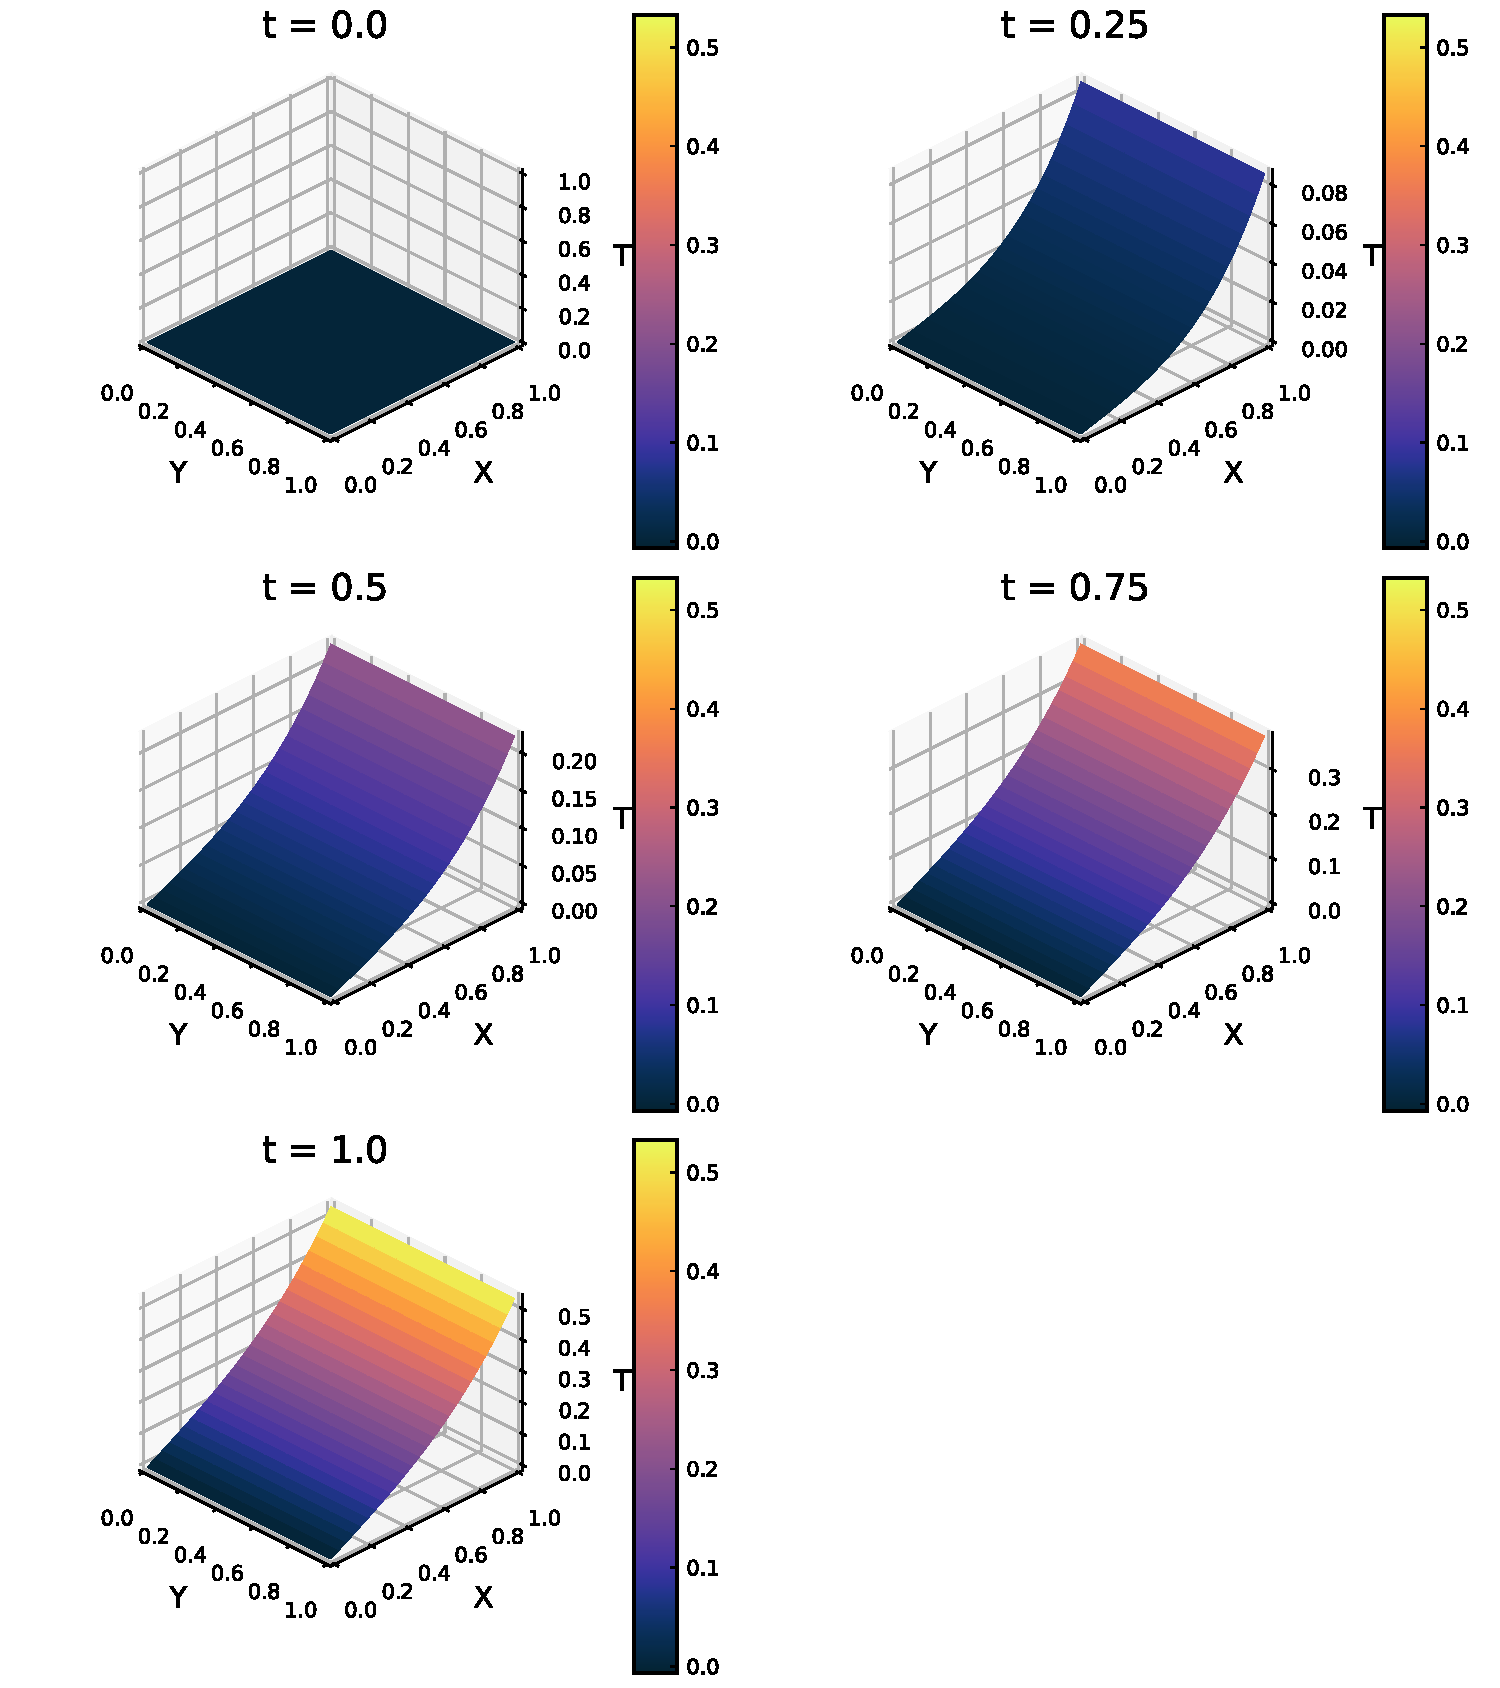
\includegraphics[keepaspectratio]{index_files/mediabag/pred_crank_nick_files/figure-pdf/fig-met-crank-nick-output-1.pdf}}

}

\caption{\label{fig-met-crank-nick}Resultados obtenidos mediante el
método numérico de Crank Nickolson.}

\end{figure}%

\section{Guardado de datos}\label{guardado-de-datos}

Con el objetivo de optimizar el proceso de comparación cuantitativa con
el modelo de redes neuronales, se exportó un subconjunto representativo
de los resultados. Aunque la simulación original utilizó una malla de
51×51 puntos, se almacenaron únicamente los valores correspondientes a
una grilla de 26×26 puntos. Esta decisión se basó en:

\begin{enumerate}
\def\labelenumi{\arabic{enumi}.}
\tightlist
\item
  Suficiencia estadística: La densidad de puntos conserva los patrones
  espaciales críticos.
\item
  Eficiencia computacional: Reduce el tamaño del archivo sin perder
  información relevante.
\end{enumerate}

Los datos se guardaron en un archivo CSV estructurado con las siguientes
columnas:

\begin{itemize}
\tightlist
\item
  Coordenadas espacio-temporales (t, x, y) para cada punto de la grilla
  26×26.
\item
  Valores de la solución en los tiempos de interés.
\end{itemize}

Este archivo permitió calcular de manera estandarizada las métricas de
error (MAE, MaxAE, error L2) en la sección de comparación de resultados.

\chapter{Métricas del modelo}\label{muxe9tricas-del-modelo}

Conforme se ha referido previamente, el desarrollo del modelo predictivo
se realizó utilizando el framework DeepXDE (versión 1.10.1) con backend
de TensorFlow 1.x (configurado mediante tensorflow.compat.v1). Para
asegurar reproducibilidad, se fijó la semilla aleatoria en 123 a nivel
de DeepXDE, TensorFlow y NumPy. La red neuronal se implementó como un
DeepONetCartesianProd con la siguiente estructura especializada:

\begin{itemize}
\tightlist
\item
  Rama (\emph{branch})

  \begin{itemize}
  \tightlist
  \item
    Capa de entrada: (num\_sensors + 1)² = 25 neuronas.
  \item
    3 capas ocultas de 20 neuronas cada una.
  \end{itemize}
\item
  Tronco (\emph{trunk})

  \begin{itemize}
  \tightlist
  \item
    Capa de entrada: 3 neuronas (coordenadas espaciotemporales x, y, t).
  \item
    Misma configuración de capas ocultas que la rama.
  \end{itemize}
\item
  Hiperparámetros clave

  \begin{itemize}
  \tightlist
  \item
    Función de activación: ELU (Exponential Linear Unit).
  \item
    Inicialización de pesos: Glorot normal.
  \item
    Optimizador: Adam con tasa de aprendizaje inicial de 2×10⁻³ y
    decaimiento exponencial (decay\_rate=0.05 cada 1000 pasos).
  \end{itemize}
\end{itemize}

\begin{Shaded}
\begin{Highlighting}[]
\ImportTok{import}\NormalTok{ deepxde }\ImportTok{as}\NormalTok{ dde}
\ImportTok{import}\NormalTok{ numpy }\ImportTok{as}\NormalTok{ np}
\ImportTok{import}\NormalTok{ tensorflow }\ImportTok{as}\NormalTok{ tf}

\CommentTok{\# {-}{-}{-}{-}{-}{-}{-}{-}{-}{-}{-}{-}{-}{-}{-}{-}{-}{-}{-}{-}{-}{-}{-}{-}{-}{-}{-}{-}{-}{-}{-}{-}{-}{-}{-}{-}{-}{-}{-}{-}{-}{-}{-}{-}{-}{-}{-}{-}{-}{-}{-}{-}{-}{-}{-}{-}{-}{-}{-}{-}{-}{-}{-}{-}{-}{-}{-}{-}{-}{-}{-}{-}{-}}
\CommentTok{\# Constants and Parameters}
\CommentTok{\# {-}{-}{-}{-}{-}{-}{-}{-}{-}{-}{-}{-}{-}{-}{-}{-}{-}{-}{-}{-}{-}{-}{-}{-}{-}{-}{-}{-}{-}{-}{-}{-}{-}{-}{-}{-}{-}{-}{-}{-}{-}{-}{-}{-}{-}{-}{-}{-}{-}{-}{-}{-}{-}{-}{-}{-}{-}{-}{-}{-}{-}{-}{-}{-}{-}{-}{-}{-}{-}{-}{-}{-}{-}}

\CommentTok{\# Backend and seed}
\NormalTok{dde.backend.set\_default\_backend(}\StringTok{"tensorflow.compat.v1"}\NormalTok{)}
\NormalTok{dde.config.set\_random\_seed(}\DecValTok{123}\NormalTok{)}

\CommentTok{\# Physical parameters}
\NormalTok{p }\OperatorTok{=} \DecValTok{1050}
\NormalTok{c }\OperatorTok{=} \DecValTok{3639}
\NormalTok{keff }\OperatorTok{=} \DecValTok{5}
\NormalTok{tf }\OperatorTok{=} \DecValTok{1800}
\NormalTok{L0 }\OperatorTok{=} \FloatTok{0.05}
\NormalTok{cb }\OperatorTok{=} \DecValTok{3825}
\NormalTok{Q }\OperatorTok{=} \DecValTok{0}
\NormalTok{TM }\OperatorTok{=} \DecValTok{45}
\NormalTok{Ta }\OperatorTok{=} \DecValTok{37}
\NormalTok{alpha }\OperatorTok{=}\NormalTok{ p }\OperatorTok{*}\NormalTok{ c }\OperatorTok{/}\NormalTok{ keff}

\CommentTok{\# Dimensionless coefficients}
\NormalTok{a1 }\OperatorTok{=}\NormalTok{ tf }\OperatorTok{/}\NormalTok{ (alpha }\OperatorTok{*}\NormalTok{ L0}\OperatorTok{**}\DecValTok{2}\NormalTok{)}
\NormalTok{a2 }\OperatorTok{=}\NormalTok{ tf }\OperatorTok{*}\NormalTok{ cb }\OperatorTok{/}\NormalTok{ (p }\OperatorTok{*}\NormalTok{ c)}
\NormalTok{a3 }\OperatorTok{=}\NormalTok{ (tf }\OperatorTok{*}\NormalTok{ Q) }\OperatorTok{/}\NormalTok{ (p }\OperatorTok{*}\NormalTok{ c }\OperatorTok{*}\NormalTok{ (TM }\OperatorTok{{-}}\NormalTok{ Ta))}

\CommentTok{\# Domain boundaries}
\NormalTok{x\_initial, x\_boundary }\OperatorTok{=} \FloatTok{0.0}\NormalTok{, }\FloatTok{1.0}
\NormalTok{y\_initial, y\_boundary }\OperatorTok{=} \FloatTok{0.0}\NormalTok{, }\FloatTok{1.0}
\NormalTok{t\_initial, t\_final }\OperatorTok{=} \FloatTok{0.0}\NormalTok{, }\FloatTok{1.0}

\CommentTok{\# Dataset configuration}
\NormalTok{pts\_dom }\OperatorTok{=} \DecValTok{30}
\NormalTok{pts\_bc }\OperatorTok{=} \DecValTok{15}
\NormalTok{pts\_ic }\OperatorTok{=} \DecValTok{30}
\NormalTok{num\_test }\OperatorTok{=} \DecValTok{25}

\CommentTok{\# Sensor grid and function space}
\NormalTok{num\_sensors }\OperatorTok{=} \DecValTok{4}
\NormalTok{size\_cov\_matrix }\OperatorTok{=} \DecValTok{40}

\CommentTok{\# Network architecture}
\NormalTok{width\_net }\OperatorTok{=} \DecValTok{30}
\NormalTok{len\_net }\OperatorTok{=} \DecValTok{3}
\NormalTok{AF }\OperatorTok{=} \StringTok{"elu"}
\NormalTok{k\_initializer }\OperatorTok{=} \StringTok{"Glorot normal"}

\CommentTok{\# Training parameters}
\NormalTok{num\_iterations }\OperatorTok{=} \DecValTok{10000}
\NormalTok{learning\_rate }\OperatorTok{=} \FloatTok{2e{-}3}
\NormalTok{decay\_rate }\OperatorTok{=} \FloatTok{0.05}
\NormalTok{decay\_steps }\OperatorTok{=} \DecValTok{1000}

\CommentTok{\# {-}{-}{-}{-}{-}{-}{-}{-}{-}{-}{-}{-}{-}{-}{-}{-}{-}{-}{-}{-}{-}{-}{-}{-}{-}{-}{-}{-}{-}{-}{-}{-}{-}{-}{-}{-}{-}{-}{-}{-}{-}{-}{-}{-}{-}{-}{-}{-}{-}{-}{-}{-}{-}{-}{-}{-}{-}{-}{-}{-}{-}{-}{-}{-}{-}{-}{-}{-}{-}{-}{-}{-}{-}}
\CommentTok{\# Geometry and Time Domain}
\CommentTok{\# {-}{-}{-}{-}{-}{-}{-}{-}{-}{-}{-}{-}{-}{-}{-}{-}{-}{-}{-}{-}{-}{-}{-}{-}{-}{-}{-}{-}{-}{-}{-}{-}{-}{-}{-}{-}{-}{-}{-}{-}{-}{-}{-}{-}{-}{-}{-}{-}{-}{-}{-}{-}{-}{-}{-}{-}{-}{-}{-}{-}{-}{-}{-}{-}{-}{-}{-}{-}{-}{-}{-}{-}{-}}

\NormalTok{spatial\_domain }\OperatorTok{=}\NormalTok{ dde.geometry.Rectangle([x\_initial, y\_initial],}
\NormalTok{                                        [x\_boundary, y\_boundary])}
\NormalTok{time\_domain }\OperatorTok{=}\NormalTok{ dde.geometry.TimeDomain(t\_initial, t\_final)}
\NormalTok{geomtime }\OperatorTok{=}\NormalTok{ dde.geometry.GeometryXTime(spatial\_domain, time\_domain)}

\CommentTok{\# {-}{-}{-}{-}{-}{-}{-}{-}{-}{-}{-}{-}{-}{-}{-}{-}{-}{-}{-}{-}{-}{-}{-}{-}{-}{-}{-}{-}{-}{-}{-}{-}{-}{-}{-}{-}{-}{-}{-}{-}{-}{-}{-}{-}{-}{-}{-}{-}{-}{-}{-}{-}{-}{-}{-}{-}{-}{-}{-}{-}{-}{-}{-}{-}{-}{-}{-}{-}{-}{-}{-}{-}{-}}
\CommentTok{\# PDE and Conditions}
\CommentTok{\# {-}{-}{-}{-}{-}{-}{-}{-}{-}{-}{-}{-}{-}{-}{-}{-}{-}{-}{-}{-}{-}{-}{-}{-}{-}{-}{-}{-}{-}{-}{-}{-}{-}{-}{-}{-}{-}{-}{-}{-}{-}{-}{-}{-}{-}{-}{-}{-}{-}{-}{-}{-}{-}{-}{-}{-}{-}{-}{-}{-}{-}{-}{-}{-}{-}{-}{-}{-}{-}{-}{-}{-}{-}}

\KeywordTok{def}\NormalTok{ initial\_condition(X):}
    \ControlFlowTok{return} \DecValTok{0}

\KeywordTok{def}\NormalTok{ heat\_equation(func, u, coords):}
\NormalTok{    u\_t }\OperatorTok{=}\NormalTok{ dde.grad.jacobian(u, func, i}\OperatorTok{=}\DecValTok{0}\NormalTok{, j}\OperatorTok{=}\DecValTok{2}\NormalTok{)}
\NormalTok{    u\_xx }\OperatorTok{=}\NormalTok{ dde.grad.hessian(u, func, i}\OperatorTok{=}\DecValTok{0}\NormalTok{, j}\OperatorTok{=}\DecValTok{0}\NormalTok{)}
\NormalTok{    u\_yy }\OperatorTok{=}\NormalTok{ dde.grad.hessian(u, func, i}\OperatorTok{=}\DecValTok{1}\NormalTok{, j}\OperatorTok{=}\DecValTok{1}\NormalTok{)}
    \ControlFlowTok{return}\NormalTok{ a1 }\OperatorTok{*}\NormalTok{ u\_t }\OperatorTok{{-}}\NormalTok{ (u\_xx }\OperatorTok{+}\NormalTok{ u\_yy) }\OperatorTok{+}\NormalTok{ a2 }\OperatorTok{*}\NormalTok{ u}

\KeywordTok{def}\NormalTok{ zero\_value(X):}
    \ControlFlowTok{return} \DecValTok{0}

\KeywordTok{def}\NormalTok{ time\_value(X):}
    \ControlFlowTok{return}\NormalTok{ X[:, }\DecValTok{2}\NormalTok{]}

\KeywordTok{def}\NormalTok{ is\_on\_vertex(x):}
\NormalTok{    vertices }\OperatorTok{=}\NormalTok{ np.array([[x\_initial, y\_initial],}
\NormalTok{                         [x\_boundary, y\_initial],}
\NormalTok{                         [x\_initial, y\_boundary],}
\NormalTok{                         [x\_boundary, y\_boundary]])}
    \ControlFlowTok{return} \BuiltInTok{any}\NormalTok{(np.allclose(x, v) }\ControlFlowTok{for}\NormalTok{ v }\KeywordTok{in}\NormalTok{ vertices)}

\KeywordTok{def}\NormalTok{ is\_initial(X, on\_initial):}
    \ControlFlowTok{return}\NormalTok{ on\_initial }\KeywordTok{and}\NormalTok{ np.isclose(X[}\DecValTok{2}\NormalTok{], t\_initial)}

\KeywordTok{def}\NormalTok{ left\_boundary(X, on\_boundary):}
\NormalTok{    spatial }\OperatorTok{=}\NormalTok{ X[}\DecValTok{0}\NormalTok{:}\DecValTok{2}\NormalTok{]}
\NormalTok{    t }\OperatorTok{=}\NormalTok{ X[}\DecValTok{2}\NormalTok{]}
    \ControlFlowTok{return}\NormalTok{ (}
\NormalTok{        on\_boundary }
        \KeywordTok{and}\NormalTok{ np.isclose(spatial[}\DecValTok{0}\NormalTok{], x\_initial) }
        \KeywordTok{and} \KeywordTok{not}\NormalTok{ np.isclose(t, t\_initial) }
        \KeywordTok{and} \KeywordTok{not}\NormalTok{ is\_on\_vertex(spatial)}
\NormalTok{    )}

\KeywordTok{def}\NormalTok{ right\_boundary(X, on\_boundary):}
\NormalTok{    spatial }\OperatorTok{=}\NormalTok{ X[}\DecValTok{0}\NormalTok{:}\DecValTok{2}\NormalTok{]}
\NormalTok{    t }\OperatorTok{=}\NormalTok{ X[}\DecValTok{2}\NormalTok{]}
    \ControlFlowTok{return}\NormalTok{ (}
\NormalTok{        on\_boundary }
        \KeywordTok{and}\NormalTok{ np.isclose(spatial[}\DecValTok{0}\NormalTok{], x\_boundary) }
        \KeywordTok{and} \KeywordTok{not}\NormalTok{ np.isclose(t, t\_initial) }
        \KeywordTok{and} \KeywordTok{not}\NormalTok{ is\_on\_vertex(spatial)}
\NormalTok{    )}

\KeywordTok{def}\NormalTok{ up\_low\_boundary(X, on\_boundary):}
\NormalTok{    spatial }\OperatorTok{=}\NormalTok{ X[}\DecValTok{0}\NormalTok{:}\DecValTok{2}\NormalTok{]}
\NormalTok{    t }\OperatorTok{=}\NormalTok{ X[}\DecValTok{2}\NormalTok{]}
    \ControlFlowTok{return}\NormalTok{ (on\_boundary }
    \KeywordTok{and}\NormalTok{ (np.isclose(spatial[}\DecValTok{1}\NormalTok{], y\_initial) }
    \KeywordTok{or}\NormalTok{ np.isclose(spatial[}\DecValTok{1}\NormalTok{], y\_boundary)) }
    \KeywordTok{and} \KeywordTok{not}\NormalTok{ np.isclose(t, t\_initial) }
    \KeywordTok{and} \KeywordTok{not}\NormalTok{ is\_on\_vertex(spatial)}
\NormalTok{    )}

\CommentTok{\# Initial and boundary conditions}
\NormalTok{ic }\OperatorTok{=}\NormalTok{ dde.icbc.IC(geomtime, initial\_condition, is\_initial)}
\NormalTok{left\_bc }\OperatorTok{=}\NormalTok{ dde.icbc.DirichletBC(geomtime, }
\NormalTok{                                zero\_value, left\_boundary)}
\NormalTok{right\_bc }\OperatorTok{=}\NormalTok{ dde.icbc.NeumannBC(geomtime,}
\NormalTok{                                time\_value, right\_boundary)}
\NormalTok{up\_low\_bc }\OperatorTok{=}\NormalTok{ dde.icbc.NeumannBC(geomtime, }
\NormalTok{                                zero\_value, up\_low\_boundary)}

\CommentTok{\# {-}{-}{-}{-}{-}{-}{-}{-}{-}{-}{-}{-}{-}{-}{-}{-}{-}{-}{-}{-}{-}{-}{-}{-}{-}{-}{-}{-}{-}{-}{-}{-}{-}{-}{-}{-}{-}{-}{-}{-}{-}{-}{-}{-}{-}{-}{-}{-}{-}{-}{-}{-}{-}{-}{-}{-}{-}{-}{-}{-}{-}{-}{-}{-}{-}{-}{-}{-}{-}{-}{-}{-}{-}}
\CommentTok{\# Dataset Construction}
\CommentTok{\# {-}{-}{-}{-}{-}{-}{-}{-}{-}{-}{-}{-}{-}{-}{-}{-}{-}{-}{-}{-}{-}{-}{-}{-}{-}{-}{-}{-}{-}{-}{-}{-}{-}{-}{-}{-}{-}{-}{-}{-}{-}{-}{-}{-}{-}{-}{-}{-}{-}{-}{-}{-}{-}{-}{-}{-}{-}{-}{-}{-}{-}{-}{-}{-}{-}{-}{-}{-}{-}{-}{-}{-}{-}}

\NormalTok{pde\_data }\OperatorTok{=}\NormalTok{ dde.data.TimePDE(}
\NormalTok{    geomtime,}
\NormalTok{    heat\_equation,}
\NormalTok{    [ic, left\_bc, right\_bc, up\_low\_bc],}
\NormalTok{    num\_domain}\OperatorTok{=}\NormalTok{pts\_dom,}
\NormalTok{    num\_boundary}\OperatorTok{=}\NormalTok{pts\_bc,}
\NormalTok{    num\_initial}\OperatorTok{=}\NormalTok{pts\_ic }
\NormalTok{)}

\CommentTok{\# {-}{-}{-}{-}{-}{-}{-}{-}{-}{-}{-}{-}{-}{-}{-}{-}{-}{-}{-}{-}{-}{-}{-}{-}{-}{-}{-}{-}{-}{-}{-}{-}{-}{-}{-}{-}{-}{-}{-}{-}{-}{-}{-}{-}{-}{-}{-}{-}{-}{-}{-}{-}{-}{-}{-}{-}{-}{-}{-}{-}{-}{-}{-}{-}{-}{-}{-}{-}{-}{-}{-}{-}{-}}
\CommentTok{\# Sensor Points and Function Space}
\CommentTok{\# {-}{-}{-}{-}{-}{-}{-}{-}{-}{-}{-}{-}{-}{-}{-}{-}{-}{-}{-}{-}{-}{-}{-}{-}{-}{-}{-}{-}{-}{-}{-}{-}{-}{-}{-}{-}{-}{-}{-}{-}{-}{-}{-}{-}{-}{-}{-}{-}{-}{-}{-}{-}{-}{-}{-}{-}{-}{-}{-}{-}{-}{-}{-}{-}{-}{-}{-}{-}{-}{-}{-}{-}{-}}

\NormalTok{side }\OperatorTok{=}\NormalTok{ np.linspace(x\_initial, x\_boundary, num\_sensors }\OperatorTok{+} \DecValTok{1}\NormalTok{)}
\NormalTok{x, y }\OperatorTok{=}\NormalTok{ np.meshgrid(side, side, indexing}\OperatorTok{=}\StringTok{\textquotesingle{}xy\textquotesingle{}}\NormalTok{)}
\NormalTok{sensor\_pts }\OperatorTok{=}\NormalTok{ np.stack([x.ravel(), y.ravel()], axis}\OperatorTok{=}\DecValTok{1}\NormalTok{)}

\NormalTok{fs }\OperatorTok{=}\NormalTok{ dde.data.function\_spaces.GRF2D(N}\OperatorTok{=}\NormalTok{size\_cov\_matrix, }
\NormalTok{                                    interp}\OperatorTok{=}\StringTok{"linear"}\NormalTok{)}

\NormalTok{data }\OperatorTok{=}\NormalTok{ dde.data.PDEOperatorCartesianProd(}
\NormalTok{    pde\_data,}
\NormalTok{    fs,}
\NormalTok{    sensor\_pts,}
\NormalTok{    num\_function}\OperatorTok{=}\DecValTok{50}\NormalTok{,}
\NormalTok{    function\_variables}\OperatorTok{=}\NormalTok{[}\DecValTok{0}\NormalTok{, }\DecValTok{1}\NormalTok{],}
\NormalTok{    num\_test}\OperatorTok{=}\NormalTok{num\_test}
\NormalTok{)}

\CommentTok{\# {-}{-}{-}{-}{-}{-}{-}{-}{-}{-}{-}{-}{-}{-}{-}{-}{-}{-}{-}{-}{-}{-}{-}{-}{-}{-}{-}{-}{-}{-}{-}{-}{-}{-}{-}{-}{-}{-}{-}{-}{-}{-}{-}{-}{-}{-}{-}{-}{-}{-}{-}{-}{-}{-}{-}{-}{-}{-}{-}{-}{-}{-}{-}{-}{-}{-}{-}{-}{-}{-}{-}{-}{-}}
\CommentTok{\# Network Definition}
\CommentTok{\# {-}{-}{-}{-}{-}{-}{-}{-}{-}{-}{-}{-}{-}{-}{-}{-}{-}{-}{-}{-}{-}{-}{-}{-}{-}{-}{-}{-}{-}{-}{-}{-}{-}{-}{-}{-}{-}{-}{-}{-}{-}{-}{-}{-}{-}{-}{-}{-}{-}{-}{-}{-}{-}{-}{-}{-}{-}{-}{-}{-}{-}{-}{-}{-}{-}{-}{-}{-}{-}{-}{-}{-}{-}}

\NormalTok{branch\_layers }\OperatorTok{=}\NormalTok{ [(num\_sensors }\OperatorTok{+} \DecValTok{1}\NormalTok{)}\OperatorTok{**}\DecValTok{2}\NormalTok{] }\OperatorTok{+}\NormalTok{ len\_net }\OperatorTok{*}\NormalTok{ [width\_net]}
\NormalTok{trunk\_layers }\OperatorTok{=}\NormalTok{ [}\DecValTok{3}\NormalTok{] }\OperatorTok{+}\NormalTok{ len\_net }\OperatorTok{*}\NormalTok{ [width\_net]}

\NormalTok{net }\OperatorTok{=}\NormalTok{ dde.nn.DeepONetCartesianProd(}
\NormalTok{    branch\_layers,}
\NormalTok{    trunk\_layers,}
\NormalTok{    activation}\OperatorTok{=}\NormalTok{AF,}
\NormalTok{    kernel\_initializer}\OperatorTok{=}\NormalTok{k\_initializer}
\NormalTok{)}

\CommentTok{\# {-}{-}{-}{-}{-}{-}{-}{-}{-}{-}{-}{-}{-}{-}{-}{-}{-}{-}{-}{-}{-}{-}{-}{-}{-}{-}{-}{-}{-}{-}{-}{-}{-}{-}{-}{-}{-}{-}{-}{-}{-}{-}{-}{-}{-}{-}{-}{-}{-}{-}{-}{-}{-}{-}{-}{-}{-}{-}{-}{-}{-}{-}{-}{-}{-}{-}{-}{-}{-}{-}{-}{-}{-}}
\CommentTok{\# Model Compilation and Training}
\CommentTok{\# {-}{-}{-}{-}{-}{-}{-}{-}{-}{-}{-}{-}{-}{-}{-}{-}{-}{-}{-}{-}{-}{-}{-}{-}{-}{-}{-}{-}{-}{-}{-}{-}{-}{-}{-}{-}{-}{-}{-}{-}{-}{-}{-}{-}{-}{-}{-}{-}{-}{-}{-}{-}{-}{-}{-}{-}{-}{-}{-}{-}{-}{-}{-}{-}{-}{-}{-}{-}{-}{-}{-}{-}{-}}

\NormalTok{model }\OperatorTok{=}\NormalTok{ dde.Model(data, net)}
\NormalTok{model.}\BuiltInTok{compile}\NormalTok{(}\StringTok{"adam"}\NormalTok{, lr}\OperatorTok{=}\NormalTok{learning\_rate,}
\NormalTok{            decay}\OperatorTok{=}\NormalTok{(}\StringTok{"inverse time"}\NormalTok{, decay\_steps, decay\_rate))}
\NormalTok{losshistory, train\_state }\OperatorTok{=}\NormalTok{ model.train(iterations}\OperatorTok{=}\NormalTok{num\_iterations)}

\CommentTok{\# Fine{-}tuning with LBFGS optimizer}
\NormalTok{model.}\BuiltInTok{compile}\NormalTok{(}\StringTok{"L{-}BFGS"}\NormalTok{)}
\NormalTok{losshistory, train\_state }\OperatorTok{=}\NormalTok{ model.train()}
\end{Highlighting}
\end{Shaded}

\section{Gráficas de pérdida del
modelo}\label{gruxe1ficas-de-puxe9rdida-del-modelo}

El proceso de entrenamiento del modelo se monitoreó mediante el
seguimiento detallado de cinco componentes de pérdida, cada una asociada
a restricciones físicas y matemáticas específicas del problema:

\begin{enumerate}
\def\labelenumi{\arabic{enumi}.}
\tightlist
\item
  Pérdida residual de la EDP

  \begin{itemize}
  \tightlist
  \item
    Función: Mide el cumplimiento de la ecuación de Bio-Calor en el
    dominio interior.
  \item
    Importancia: Garantiza que la solución aprendida satisfaga la física
    subyacente.
  \item
    Comportamiento esperado: Debe converger a valores cercanos a cero
    (típicamente \textless{} 1e-3).
  \end{itemize}
\item
  Pérdida de condición inicial

  \begin{itemize}
  \tightlist
  \item
    Función: Controla la precisión en t=0.
  \item
    Importancia: Asegura coherencia con el estado inicial del sistema.
  \item
    Patrón típico: Suele ser la primera en converger por su carácter
    puntual.
  \end{itemize}
\item
  Pérdida de frontera izquierda (Dirichlet)

  \begin{itemize}
  \tightlist
  \item
    Función: Evalúa el cumplimiento de condiciones de valor prescrito.
  \item
    Relevancia: Mantiene valores fijos en bordes específicos.
  \item
    Convergencia: Normalmente rápida por ser restrictiva.
  \end{itemize}
\item
  Pérdida de frontera derecha (Neumann)

  \begin{itemize}
  \tightlist
  \item
    Función: Verifica gradientes normales en esta frontera
  \item
    Dificultad característica: Puede mostrar oscilaciones iniciales
  \end{itemize}
\item
  Pérdida de fronteras superior/inferior (Neumann)

  \begin{itemize}
  \tightlist
  \item
    Función: Controla condiciones de flujo en estos bordes
  \item
    Complejidad: En problemas 2D/3D suele ser la última en estabilizarse
  \end{itemize}
\end{enumerate}

\subsection{Perdida para el conjunto de
entrenamiento}\label{perdida-para-el-conjunto-de-entrenamiento}

\begin{Shaded}
\begin{Highlighting}[]
\ImportTok{import}\NormalTok{ plotly.graph\_objects }\ImportTok{as}\NormalTok{ go}

\CommentTok{\# Nombres de las componentes del loss}
\NormalTok{loss\_labels }\OperatorTok{=}\NormalTok{ [}
    \StringTok{"Pérdida residual PDE"}\NormalTok{,}
    \StringTok{"Pérdida de condición inicial"}\NormalTok{,}
    \StringTok{"Pérdida de frontera izquierda (Dirichlet)"}\NormalTok{,}
    \StringTok{"Pérdida de frontera derecha (Neumann)"}\NormalTok{,}
    \StringTok{"Pérdida de fronteras superior/inferior (Neumann)"}
\NormalTok{]}

\CommentTok{\# Extraer pasos y pérdida de entrenamiento}
\NormalTok{steps }\OperatorTok{=}\NormalTok{ losshistory.steps}
\NormalTok{train\_loss }\OperatorTok{=}\NormalTok{ np.array(losshistory.loss\_train)}

\CommentTok{\# Crear figura}
\NormalTok{fig\_train }\OperatorTok{=}\NormalTok{ go.Figure()}

\ControlFlowTok{for}\NormalTok{ i }\KeywordTok{in} \BuiltInTok{range}\NormalTok{(train\_loss.shape[}\DecValTok{1}\NormalTok{]):}
\NormalTok{    fig\_train.add\_trace(go.Scatter(}
\NormalTok{        x}\OperatorTok{=}\NormalTok{steps,}
\NormalTok{        y}\OperatorTok{=}\NormalTok{train\_loss[:, i],}
\NormalTok{        mode}\OperatorTok{=}\StringTok{\textquotesingle{}lines\textquotesingle{}}\NormalTok{,}
\NormalTok{        name}\OperatorTok{=}\NormalTok{loss\_labels[i]}
\NormalTok{    ))}

\NormalTok{fig\_train.update\_layout(}
\NormalTok{    title}\OperatorTok{=}\StringTok{"Historial de pérdida en el entrenamiento"}\NormalTok{,}
\NormalTok{    xaxis}\OperatorTok{=}\BuiltInTok{dict}\NormalTok{(title}\OperatorTok{=}\StringTok{"Iteración"}\NormalTok{, tickformat}\OperatorTok{=}\StringTok{".1e"}\NormalTok{),}
\NormalTok{    yaxis}\OperatorTok{=}\BuiltInTok{dict}\NormalTok{(title}\OperatorTok{=}\StringTok{"Pérdida (log)"}\NormalTok{, }\BuiltInTok{type}\OperatorTok{=}\StringTok{"log"}\NormalTok{, tickformat}\OperatorTok{=}\StringTok{".1e"}\NormalTok{),}
\NormalTok{    template}\OperatorTok{=}\StringTok{"plotly\_white"}\NormalTok{,}
\NormalTok{    legend}\OperatorTok{=}\BuiltInTok{dict}\NormalTok{(x}\OperatorTok{=}\FloatTok{0.99}\NormalTok{, y}\OperatorTok{=}\FloatTok{0.99}\NormalTok{),}
\NormalTok{    font}\OperatorTok{=}\BuiltInTok{dict}\NormalTok{(size}\OperatorTok{=}\DecValTok{14}\NormalTok{)}
\NormalTok{)}
\end{Highlighting}
\end{Shaded}

\begin{figure}

\centering{

\pandocbounded{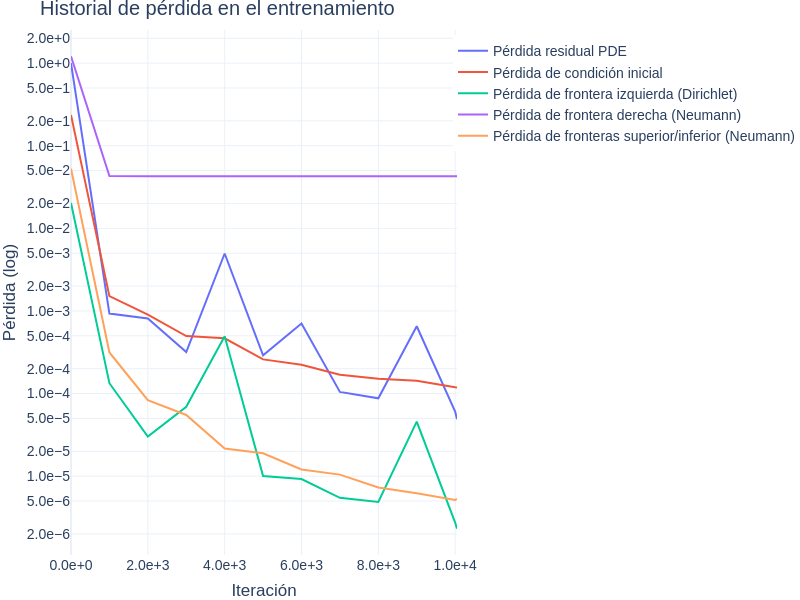
\includegraphics[keepaspectratio]{images/fig-training_loss.png}}

}

\caption{\label{fig-loss_training}Gráfica de la perdida en el
entrenamiento.}

\end{figure}%

\subsection{Pérdida para el conjunto de
prueba}\label{puxe9rdida-para-el-conjunto-de-prueba}

\begin{Shaded}
\begin{Highlighting}[]
\ImportTok{import}\NormalTok{ plotly.graph\_objects }\ImportTok{as}\NormalTok{ go}

\CommentTok{\# Nombres de las componentes del loss}
\NormalTok{loss\_labels }\OperatorTok{=}\NormalTok{ [}
    \StringTok{"Pérdida residual PDE"}\NormalTok{,}
    \StringTok{"Pérdida de condición inicial"}\NormalTok{,}
    \StringTok{"Pérdida de frontera izquierda (Dirichlet)"}\NormalTok{,}
    \StringTok{"Pérdida de frontera derecha (Neumann)"}\NormalTok{,}
    \StringTok{"Pérdida de fronteras superior/inferior (Neumann)"}
\NormalTok{]}

\CommentTok{\# Extraer pasos y pérdida de entrenamiento}
\NormalTok{steps }\OperatorTok{=}\NormalTok{ losshistory.steps}
\NormalTok{test\_loss }\OperatorTok{=}\NormalTok{ np.array(losshistory.loss\_test)}

\CommentTok{\# Crear figura}
\NormalTok{fig\_test }\OperatorTok{=}\NormalTok{ go.Figure()}

\ControlFlowTok{for}\NormalTok{ i }\KeywordTok{in} \BuiltInTok{range}\NormalTok{(test\_loss.shape[}\DecValTok{1}\NormalTok{]):}
\NormalTok{    fig\_test.add\_trace(go.Scatter(}
\NormalTok{        x}\OperatorTok{=}\NormalTok{steps,}
\NormalTok{        y}\OperatorTok{=}\NormalTok{test\_loss[:, i],}
\NormalTok{        mode}\OperatorTok{=}\StringTok{\textquotesingle{}lines\textquotesingle{}}\NormalTok{,}
\NormalTok{        name}\OperatorTok{=}\NormalTok{loss\_labels[i]}
\NormalTok{    ))}

\NormalTok{fig\_test.update\_layout(}
\NormalTok{    title}\OperatorTok{=}\StringTok{"Historial de pérdida en el conjunto de prueba"}\NormalTok{,}
\NormalTok{    xaxis}\OperatorTok{=}\BuiltInTok{dict}\NormalTok{(title}\OperatorTok{=}\StringTok{"Iteración"}\NormalTok{, tickformat}\OperatorTok{=}\StringTok{".1e"}\NormalTok{),}
\NormalTok{    yaxis}\OperatorTok{=}\BuiltInTok{dict}\NormalTok{(title}\OperatorTok{=}\StringTok{"Pérdida (log)"}\NormalTok{, }\BuiltInTok{type}\OperatorTok{=}\StringTok{"log"}\NormalTok{, tickformat}\OperatorTok{=}\StringTok{".1e"}\NormalTok{),}
\NormalTok{    template}\OperatorTok{=}\StringTok{"plotly\_white"}\NormalTok{,}
\NormalTok{    legend}\OperatorTok{=}\BuiltInTok{dict}\NormalTok{(x}\OperatorTok{=}\FloatTok{0.99}\NormalTok{, y}\OperatorTok{=}\FloatTok{0.99}\NormalTok{),}
\NormalTok{    font}\OperatorTok{=}\BuiltInTok{dict}\NormalTok{(size}\OperatorTok{=}\DecValTok{14}\NormalTok{)}
\NormalTok{)}
\end{Highlighting}
\end{Shaded}

\begin{figure}

\centering{

\pandocbounded{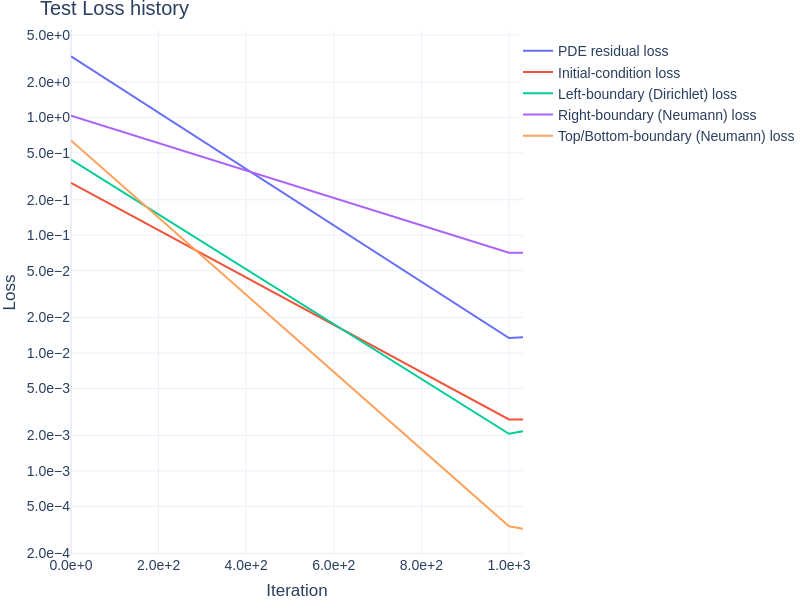
\includegraphics[keepaspectratio]{images/fig-test_loss.png}}

}

\caption{\label{fig-loss_test}Gráfica de la perdida en el conjunto de
prueba.}

\end{figure}%

\section{Guardado de datos}\label{guardado-de-datos-1}

Para permitir la comparación cuantitativa con el método de
Crank-Nicolson y facilitar la generación de visualizaciones
consistentes, se exportaron las predicciones del modelo neuronal en
formato CSV. El proceso consistió en:

\begin{enumerate}
\def\labelenumi{\arabic{enumi}.}
\tightlist
\item
  Generación de la malla de evaluación:

  \begin{itemize}
  \tightlist
  \item
    Dominio espacial: Cuadrado unitario {[}0,1{]} × {[}0,1{]}.
  \item
    Discretización: 26 segmentos equiespaciados en cada eje (x, y).
  \item
    Puntos totales: 676 (26 × 26).
  \item
    Tiempos evaluados: t = {[}0.0, 0.25, 0.50, 0.75, 1.0{]}.
  \end{itemize}
\item
  Estructura del archivo:

  \begin{itemize}
  \tightlist
  \item
    Coordenadas espacio-temporales (t, x, y) para cada punto de la
    grilla 26×26.
  \item
    Valores de la solución en los tiempos de interés.
  \end{itemize}
\end{enumerate}

\begin{Shaded}
\begin{Highlighting}[]
\ImportTok{import}\NormalTok{ pandas }\ImportTok{as}\NormalTok{ pd}
\CommentTok{\# Lista de tiempos}
\NormalTok{times }\OperatorTok{=}\NormalTok{ [}\FloatTok{0.0}\NormalTok{, }\FloatTok{0.25}\NormalTok{, }\FloatTok{0.5}\NormalTok{, }\FloatTok{0.75}\NormalTok{, }\FloatTok{1.0}\NormalTok{]}

\CommentTok{\# Crear la malla (x, y)}
\NormalTok{num\_points }\OperatorTok{=} \DecValTok{26}
\NormalTok{x }\OperatorTok{=}\NormalTok{ np.linspace(}\DecValTok{0}\NormalTok{, }\DecValTok{1}\NormalTok{, num\_points)}
\NormalTok{y }\OperatorTok{=}\NormalTok{ np.linspace(}\DecValTok{0}\NormalTok{, }\DecValTok{1}\NormalTok{, num\_points)}
\NormalTok{X, Y }\OperatorTok{=}\NormalTok{ np.meshgrid(x, y)}

\CommentTok{\# Lista para almacenar resultados}
\NormalTok{results }\OperatorTok{=}\NormalTok{ []}

\ControlFlowTok{for}\NormalTok{ t\_val }\KeywordTok{in}\NormalTok{ times:}
    \CommentTok{\# Crear entrada trunk: (num\_points\^{}2, 3)}
\NormalTok{    points }\OperatorTok{=}\NormalTok{ np.vstack((X.flatten(), Y.flatten(),}
\NormalTok{                         t\_val }\OperatorTok{*}\NormalTok{ np.ones\_like(X.flatten()))).T}

    \CommentTok{\# Crear entrada branch: condición inicial constante cero}
\NormalTok{    branch\_input }\OperatorTok{=}\NormalTok{ np.zeros((}\DecValTok{1}\NormalTok{, sensor\_pts.shape[}\DecValTok{0}\NormalTok{]))}

    \CommentTok{\# Predecir}
\NormalTok{    predicted }\OperatorTok{=}\NormalTok{ model.predict((branch\_input, points)).flatten()}

    \CommentTok{\# Agregar los datos al resultado}
    \ControlFlowTok{for}\NormalTok{ xi, yi, thetai }\KeywordTok{in} \BuiltInTok{zip}\NormalTok{(points[:, }\DecValTok{0}\NormalTok{], points[:, }\DecValTok{1}\NormalTok{], predicted):}
\NormalTok{        results.append([t\_val, xi, yi, thetai])}

\CommentTok{\# Crear el DataFrame}
\NormalTok{df }\OperatorTok{=}\NormalTok{ pd.DataFrame(results, columns}\OperatorTok{=}\NormalTok{[}\StringTok{"time"}\NormalTok{, }\StringTok{"X"}\NormalTok{, }\StringTok{"Y"}\NormalTok{, }\StringTok{"Theta"}\NormalTok{])}

\CommentTok{\# Obtener la ruta del script actual y guardar el archivo CSV}
\NormalTok{ruta }\OperatorTok{=} \VerbatimStringTok{r"data/model\_DoN}\DecValTok{.}\VerbatimStringTok{csv"}
\NormalTok{df.to\_csv(ruta, index}\OperatorTok{=}\VariableTok{False}\NormalTok{)}
\end{Highlighting}
\end{Shaded}

\chapter{Comparación de
resultados}\label{comparaciuxf3n-de-resultados-1}

\section{Comparativa visual de las
predicciones}\label{comparativa-visual-de-las-predicciones}

Esta sección presenta un análisis cualitativo de los resultados mediante
la comparación directa entre las predicciones del modelo, las soluciones
reportadas en el estudio de Alessio Borgi
(\citeproc{ref-medical_rep}{2023}) y las obtenidas mediante el método de
Crank Nickolson. La visualización paralela permite evaluar:

\begin{itemize}
\tightlist
\item
  Dominio espacial: Cuadrado unitario {[}0,1{]} × {[}0,1{]} con malla
  26×26.
\item
  Escala de colores: Mapa térmico viridis (consistente en ambas
  columnas).
\end{itemize}

\subsection{\texorpdfstring{Modelo contra resultados de Alessio Borgi
(\citeproc{ref-medical_rep}{2023})}{Modelo contra resultados de Alessio Borgi (2023)}}\label{modelo-contra-resultados-de-medical_rep}

\begin{Shaded}
\begin{Highlighting}[]
\ImportTok{import}\NormalTok{ matplotlib.pyplot }\ImportTok{as}\NormalTok{ plt}
\ImportTok{from}\NormalTok{ mpl\_toolkits.mplot3d }\ImportTok{import}\NormalTok{ Axes3D}
\ImportTok{import}\NormalTok{ matplotlib.gridspec }\ImportTok{as}\NormalTok{ gridspec}
\ImportTok{import}\NormalTok{ pandas }\ImportTok{as}\NormalTok{ pd}
\ImportTok{import}\NormalTok{ numpy }\ImportTok{as}\NormalTok{ np}

\CommentTok{\# Lista de tiempos}
\NormalTok{times }\OperatorTok{=}\NormalTok{ [}\FloatTok{0.0}\NormalTok{, }\FloatTok{0.25}\NormalTok{, }\FloatTok{0.5}\NormalTok{, }\FloatTok{0.75}\NormalTok{, }\FloatTok{1.0}\NormalTok{]}

\CommentTok{\# Cargar el dataframe}
\NormalTok{df }\OperatorTok{=}\NormalTok{ pd.read\_csv(}\VerbatimStringTok{r\textquotesingle{}data/model\_DoN}\DecValTok{.}\VerbatimStringTok{csv\textquotesingle{}}\NormalTok{)  }

\CommentTok{\# Crear figura con subplots 3D en 1 fila y 5 columnas}
\NormalTok{fig, axes }\OperatorTok{=}\NormalTok{ plt.subplots(nrows}\OperatorTok{=}\DecValTok{1}\NormalTok{, ncols}\OperatorTok{=}\BuiltInTok{len}\NormalTok{(times), }
\NormalTok{                        figsize}\OperatorTok{=}\NormalTok{(}\DecValTok{22}\NormalTok{, }\DecValTok{6}\NormalTok{),}
\NormalTok{                        subplot\_kw}\OperatorTok{=}\NormalTok{\{}\StringTok{\textquotesingle{}projection\textquotesingle{}}\NormalTok{: }\StringTok{\textquotesingle{}3d\textquotesingle{}}\NormalTok{\})}

\CommentTok{\# Asumimos que el grid es regular}
\NormalTok{num\_points }\OperatorTok{=} \BuiltInTok{int}\NormalTok{(np.sqrt(df[df[}\StringTok{"time"}\NormalTok{] }\OperatorTok{==}\NormalTok{ times[}\DecValTok{0}\NormalTok{]].shape[}\DecValTok{0}\NormalTok{]))}

\CommentTok{\# Lista para almacenar los objetos surface}
\NormalTok{surf\_list }\OperatorTok{=}\NormalTok{ []}

\CommentTok{\# Reordenar para graficar}
\ControlFlowTok{for}\NormalTok{ i, (t\_val, ax) }\KeywordTok{in} \BuiltInTok{enumerate}\NormalTok{(}\BuiltInTok{zip}\NormalTok{(times, axes)):}
    \CommentTok{\# Filtrar por tiempo actual}
\NormalTok{    df\_t }\OperatorTok{=}\NormalTok{ df[df[}\StringTok{"time"}\NormalTok{] }\OperatorTok{==}\NormalTok{ t\_val]}

    \CommentTok{\# Obtener los valores de X, Y, Theta}
\NormalTok{    X\_vals }\OperatorTok{=}\NormalTok{ df\_t[}\StringTok{"X"}\NormalTok{].values.reshape((num\_points, num\_points))}
\NormalTok{    Y\_vals }\OperatorTok{=}\NormalTok{ df\_t[}\StringTok{"Y"}\NormalTok{].values.reshape((num\_points, num\_points))}
\NormalTok{    Z\_vals }\OperatorTok{=}\NormalTok{ df\_t[}\StringTok{"Theta"}\NormalTok{].values.reshape((num\_points, num\_points))}

    \CommentTok{\# Dibujar la superficie}
\NormalTok{    surf }\OperatorTok{=}\NormalTok{ ax.plot\_surface(}
\NormalTok{        Y\_vals, X\_vals, Z\_vals,}
\NormalTok{        rstride}\OperatorTok{=}\DecValTok{1}\NormalTok{, cstride}\OperatorTok{=}\DecValTok{1}\NormalTok{,}
\NormalTok{        cmap}\OperatorTok{=}\StringTok{"YlGnBu"}\NormalTok{,}
\NormalTok{        edgecolor}\OperatorTok{=}\StringTok{"none"}\NormalTok{,}
\NormalTok{        antialiased}\OperatorTok{=}\VariableTok{True}
\NormalTok{    )}
\NormalTok{    surf\_list.append(surf)}

\NormalTok{    ax.set\_title(}\SpecialStringTok{f"Time = }\SpecialCharTok{\{}\NormalTok{t\_val}\SpecialCharTok{:.2f\}}\SpecialStringTok{ s"}\NormalTok{, pad}\OperatorTok{=}\DecValTok{10}\NormalTok{)}
\NormalTok{    ax.set\_xlabel(}\StringTok{"Y"}\NormalTok{, labelpad}\OperatorTok{=}\DecValTok{10}\NormalTok{)}
\NormalTok{    ax.set\_ylabel(}\StringTok{"X"}\NormalTok{, labelpad}\OperatorTok{=}\DecValTok{10}\NormalTok{)}
\NormalTok{    ax.set\_zlabel(}\StringTok{"T [K]"}\NormalTok{, labelpad}\OperatorTok{=}\DecValTok{10}\NormalTok{, rotation}\OperatorTok{=}\DecValTok{90}\NormalTok{)}


\CommentTok{\# Añadir barra de color común}
\NormalTok{cbar }\OperatorTok{=}\NormalTok{ fig.colorbar(surf\_list[}\OperatorTok{{-}}\DecValTok{1}\NormalTok{], ax}\OperatorTok{=}\NormalTok{axes,}
\NormalTok{                    shrink}\OperatorTok{=}\FloatTok{0.9}\NormalTok{, aspect}\OperatorTok{=}\DecValTok{90}\NormalTok{,}
\NormalTok{                    pad}\OperatorTok{=}\FloatTok{0.1}\NormalTok{, orientation}\OperatorTok{=}\StringTok{\textquotesingle{}horizontal\textquotesingle{}}\NormalTok{)}
\NormalTok{cbar.set\_label(}\StringTok{\textquotesingle{}Temperatura [K]\textquotesingle{}}\NormalTok{)}

\NormalTok{plt.show()}
\end{Highlighting}
\end{Shaded}

\begin{figure}[H]

\centering{

\pandocbounded{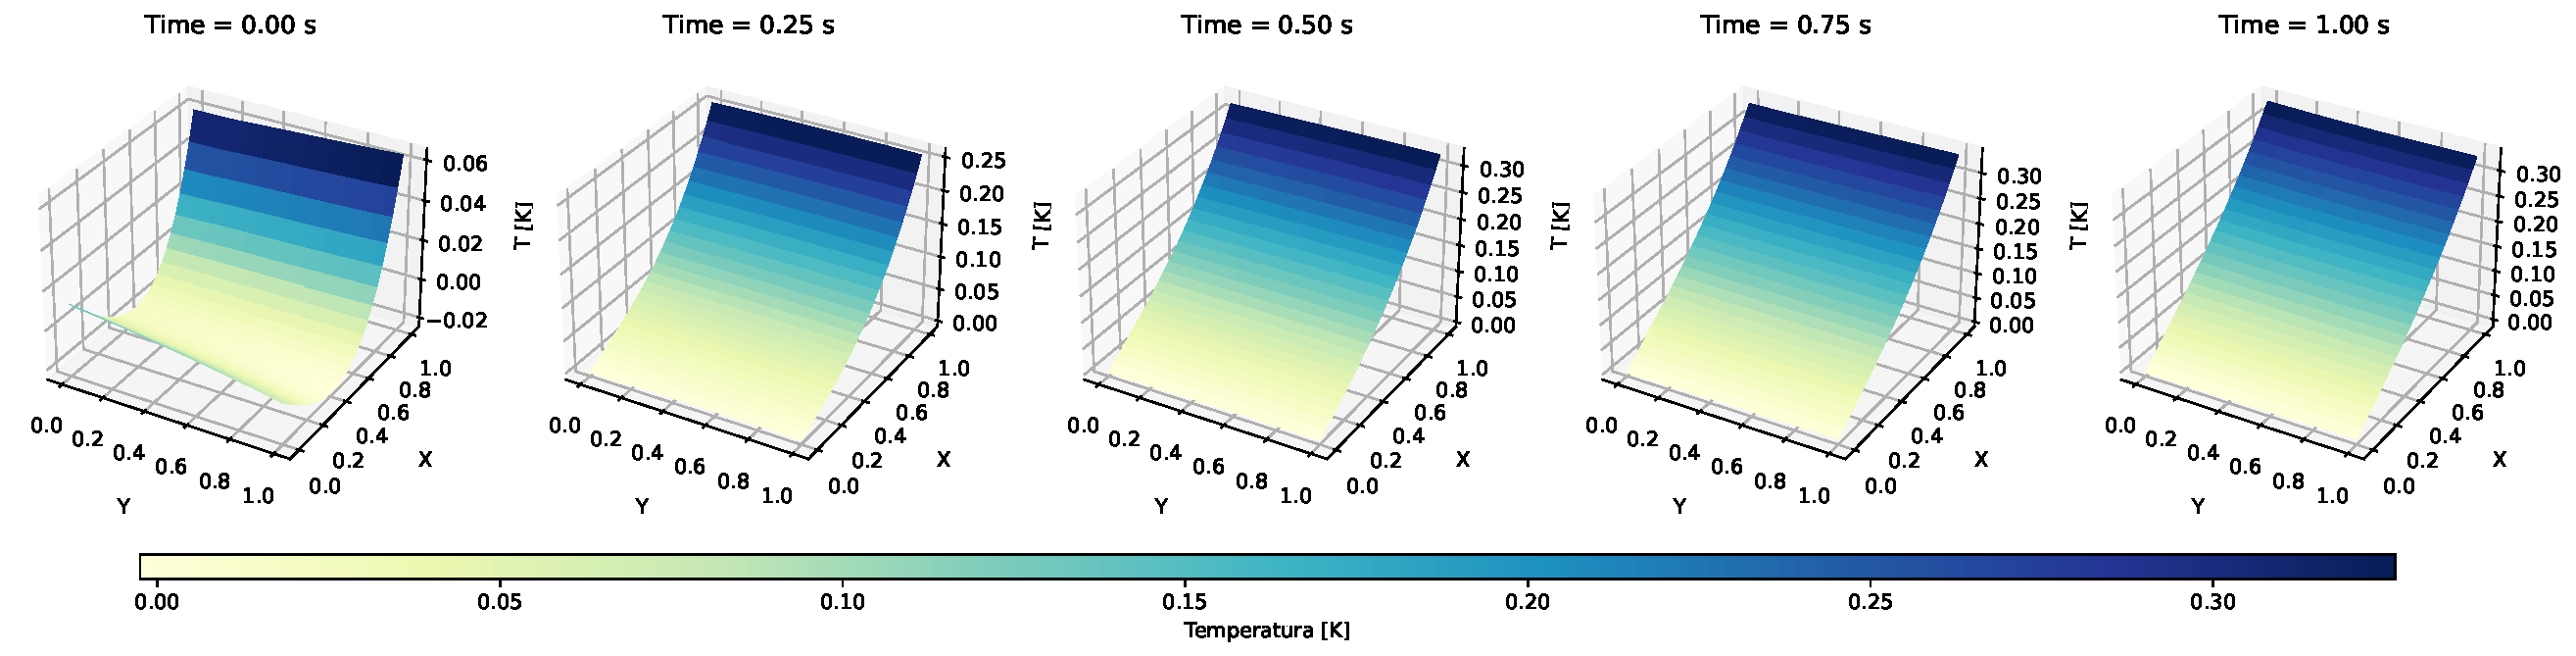
\includegraphics[keepaspectratio]{comparaciones_files/figure-pdf/fig-my_results-output-1.pdf}}

}

\caption{\label{fig-my_results}Predicciones de la red neuronal a
distintos tiempos.}

\end{figure}%

\begin{figure}

\centering{

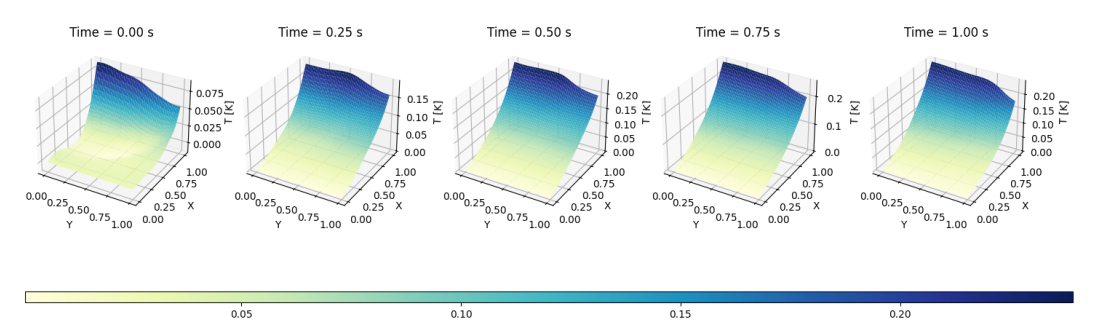
\includegraphics[width=5.72917in,height=\textheight,keepaspectratio]{images/results_paper.png}

}

\caption{\label{fig-results_fnn}Resultados reportados por Alessio Borgi
(\citeproc{ref-medical_rep}{2023}) en el caso 2D.}

\end{figure}%

\subsection{Modelo contra método
numérico}\label{modelo-contra-muxe9todo-numuxe9rico}

\begin{Shaded}
\begin{Highlighting}[]
\NormalTok{crank\_nick\_data }\OperatorTok{=}\NormalTok{ pd.read\_csv(}\VerbatimStringTok{r\textquotesingle{}data/crank\_nick}\DecValTok{.}\VerbatimStringTok{csv\textquotesingle{}}\NormalTok{)}
\NormalTok{model\_don\_data }\OperatorTok{=}\NormalTok{ pd.read\_csv(}\VerbatimStringTok{r\textquotesingle{}data/model\_DoN}\DecValTok{.}\VerbatimStringTok{csv\textquotesingle{}}\NormalTok{)}

\CommentTok{\# Determinar los límites comunes para el colorbar}
\NormalTok{min\_temp }\OperatorTok{=} \BuiltInTok{min}\NormalTok{(model\_don\_data[}\StringTok{\textquotesingle{}Theta\textquotesingle{}}\NormalTok{].}\BuiltInTok{min}\NormalTok{(),}
\NormalTok{                crank\_nick\_data[}\StringTok{\textquotesingle{}Theta\textquotesingle{}}\NormalTok{].}\BuiltInTok{min}\NormalTok{())}
\NormalTok{max\_temp }\OperatorTok{=} \BuiltInTok{max}\NormalTok{(model\_don\_data[}\StringTok{\textquotesingle{}Theta\textquotesingle{}}\NormalTok{].}\BuiltInTok{max}\NormalTok{(), }
\NormalTok{                crank\_nick\_data[}\StringTok{\textquotesingle{}Theta\textquotesingle{}}\NormalTok{].}\BuiltInTok{max}\NormalTok{())}

\CommentTok{\# Crear figura con subplots 3D en 2 filas y 5 columnas}
\NormalTok{fig }\OperatorTok{=}\NormalTok{ plt.figure(figsize}\OperatorTok{=}\NormalTok{(}\DecValTok{22}\NormalTok{, }\DecValTok{12}\NormalTok{))}
\NormalTok{axes }\OperatorTok{=}\NormalTok{ []}

\CommentTok{\# Crear los subplots}
\ControlFlowTok{for}\NormalTok{ i }\KeywordTok{in} \BuiltInTok{range}\NormalTok{(}\DecValTok{2}\NormalTok{):  }\CommentTok{\# 2 filas}
    \ControlFlowTok{for}\NormalTok{ j }\KeywordTok{in} \BuiltInTok{range}\NormalTok{(}\DecValTok{5}\NormalTok{):  }\CommentTok{\# 5 columnas}
\NormalTok{        axes.append(fig.add\_subplot(}\DecValTok{2}\NormalTok{, }\DecValTok{5}\NormalTok{, i}\OperatorTok{*}\DecValTok{5} \OperatorTok{+}\NormalTok{ j }\OperatorTok{+} \DecValTok{1}\NormalTok{, projection}\OperatorTok{=}\StringTok{\textquotesingle{}3d\textquotesingle{}}\NormalTok{))}

\NormalTok{axes }\OperatorTok{=}\NormalTok{ np.array(axes).reshape(}\DecValTok{2}\NormalTok{, }\DecValTok{5}\NormalTok{)}

\CommentTok{\# Añadir títulos generales para cada fila}
\NormalTok{fig.text(}\FloatTok{0.5}\NormalTok{, }\FloatTok{0.92}\NormalTok{, }\StringTok{"Predicciones modelo DON"}\NormalTok{, }
\NormalTok{        ha}\OperatorTok{=}\StringTok{\textquotesingle{}center\textquotesingle{}}\NormalTok{, va}\OperatorTok{=}\StringTok{\textquotesingle{}center\textquotesingle{}}\NormalTok{, fontsize}\OperatorTok{=}\DecValTok{14}\NormalTok{,fontweight}\OperatorTok{=}\StringTok{\textquotesingle{}bold\textquotesingle{}}\NormalTok{)}
\NormalTok{fig.text(}\FloatTok{0.5}\NormalTok{, }\FloatTok{0.56}\NormalTok{, }\StringTok{"Predicciones método numérico"}\NormalTok{,}
\NormalTok{        ha}\OperatorTok{=}\StringTok{\textquotesingle{}center\textquotesingle{}}\NormalTok{, va}\OperatorTok{=}\StringTok{\textquotesingle{}center\textquotesingle{}}\NormalTok{, fontsize}\OperatorTok{=}\DecValTok{14}\NormalTok{, fontweight}\OperatorTok{=}\StringTok{\textquotesingle{}bold\textquotesingle{}}\NormalTok{)}

\CommentTok{\# Función para graficar un dataframe en una fila específica}
\KeywordTok{def}\NormalTok{ plot\_dataframe(df, row, num\_points, cmap}\OperatorTok{=}\StringTok{"viridis"}\NormalTok{):}
\NormalTok{    surf\_list }\OperatorTok{=}\NormalTok{ []}
    \ControlFlowTok{for}\NormalTok{ col, t\_val }\KeywordTok{in} \BuiltInTok{enumerate}\NormalTok{(times):}
\NormalTok{        ax }\OperatorTok{=}\NormalTok{ axes[row, col]}
        
        \CommentTok{\# Filtrar por tiempo actual}
\NormalTok{        df\_t }\OperatorTok{=}\NormalTok{ df[df[}\StringTok{"time"}\NormalTok{] }\OperatorTok{==}\NormalTok{ t\_val]}

        \CommentTok{\# Obtener los valores de X, Y, Theta}
\NormalTok{        X\_vals }\OperatorTok{=}\NormalTok{ df\_t[}\StringTok{"X"}\NormalTok{].values.reshape((num\_points, num\_points))}
\NormalTok{        Y\_vals }\OperatorTok{=}\NormalTok{ df\_t[}\StringTok{"Y"}\NormalTok{].values.reshape((num\_points, num\_points))}
\NormalTok{        Z\_vals }\OperatorTok{=}\NormalTok{ df\_t[}\StringTok{"Theta"}\NormalTok{].values.reshape((num\_points, num\_points))}

        \CommentTok{\# Dibujar la superficie con límites comunes}
\NormalTok{        surf }\OperatorTok{=}\NormalTok{ ax.plot\_surface(}
\NormalTok{            Y\_vals, X\_vals, Z\_vals,}
\NormalTok{            rstride}\OperatorTok{=}\DecValTok{1}\NormalTok{, cstride}\OperatorTok{=}\DecValTok{1}\NormalTok{,}
\NormalTok{            cmap}\OperatorTok{=}\NormalTok{cmap,}
\NormalTok{            edgecolor}\OperatorTok{=}\StringTok{"none"}\NormalTok{,}
\NormalTok{            antialiased}\OperatorTok{=}\VariableTok{True}\NormalTok{,}
\NormalTok{            vmin}\OperatorTok{=}\NormalTok{min\_temp,}
\NormalTok{            vmax}\OperatorTok{=}\NormalTok{max\_temp}
\NormalTok{        )}
\NormalTok{        surf\_list.append(surf)}

\NormalTok{        ax.set\_title(}\SpecialStringTok{f"Time = }\SpecialCharTok{\{}\NormalTok{t\_val}\SpecialCharTok{:.2f\}}\SpecialStringTok{ s"}\NormalTok{, pad}\OperatorTok{=}\DecValTok{10}\NormalTok{)}
\NormalTok{        ax.set\_xlabel(}\StringTok{"Y"}\NormalTok{, labelpad}\OperatorTok{=}\DecValTok{10}\NormalTok{)}
\NormalTok{        ax.set\_ylabel(}\StringTok{"X"}\NormalTok{, labelpad}\OperatorTok{=}\DecValTok{10}\NormalTok{)}
\NormalTok{        ax.set\_zlabel(}\StringTok{"T [K]"}\NormalTok{, labelpad}\OperatorTok{=}\DecValTok{10}\NormalTok{, rotation}\OperatorTok{=}\DecValTok{90}\NormalTok{)}
    
    \ControlFlowTok{return}\NormalTok{ surf\_list}

\CommentTok{\# Asumimos que el grid es regular para ambos dataframes}
\NormalTok{num\_points }\OperatorTok{=} \BuiltInTok{int}\NormalTok{(np.sqrt(}
\NormalTok{        model\_don\_data[model\_don\_data[}\StringTok{"time"}\NormalTok{] }\OperatorTok{==}\NormalTok{ times[}\DecValTok{0}\NormalTok{]].shape[}\DecValTok{0}\NormalTok{]))}

\CommentTok{\# Graficar el primer dataframe en la fila superior}
\NormalTok{surf\_model\_don }\OperatorTok{=}\NormalTok{ plot\_dataframe(model\_don\_data, }\DecValTok{0}\NormalTok{, num\_points)}

\CommentTok{\# Graficar el segundo dataframe en la fila inferior}
\NormalTok{surf\_crank\_nick }\OperatorTok{=}\NormalTok{ plot\_dataframe(crank\_nick\_data, }\DecValTok{1}\NormalTok{, num\_points)}

\CommentTok{\# Añadir barra de color común en la parte inferior}
\NormalTok{cbar }\OperatorTok{=}\NormalTok{ fig.colorbar(surf\_crank\_nick[}\OperatorTok{{-}}\DecValTok{1}\NormalTok{], ax}\OperatorTok{=}\NormalTok{axes.ravel().tolist(),}
\NormalTok{                    use\_gridspec}\OperatorTok{=}\VariableTok{True}\NormalTok{, orientation}\OperatorTok{=}\StringTok{\textquotesingle{}horizontal\textquotesingle{}}\NormalTok{,}
\NormalTok{                    pad}\OperatorTok{=}\FloatTok{0.05}\NormalTok{, aspect}\OperatorTok{=}\DecValTok{90}\NormalTok{, shrink}\OperatorTok{=}\FloatTok{0.9}\NormalTok{)}
\NormalTok{cbar.set\_label(}\StringTok{\textquotesingle{}Temperatura [K]\textquotesingle{}}\NormalTok{, labelpad}\OperatorTok{=}\DecValTok{10}\NormalTok{)}


\NormalTok{plt.show()}
\end{Highlighting}
\end{Shaded}

\begin{figure}[H]

\centering{

\pandocbounded{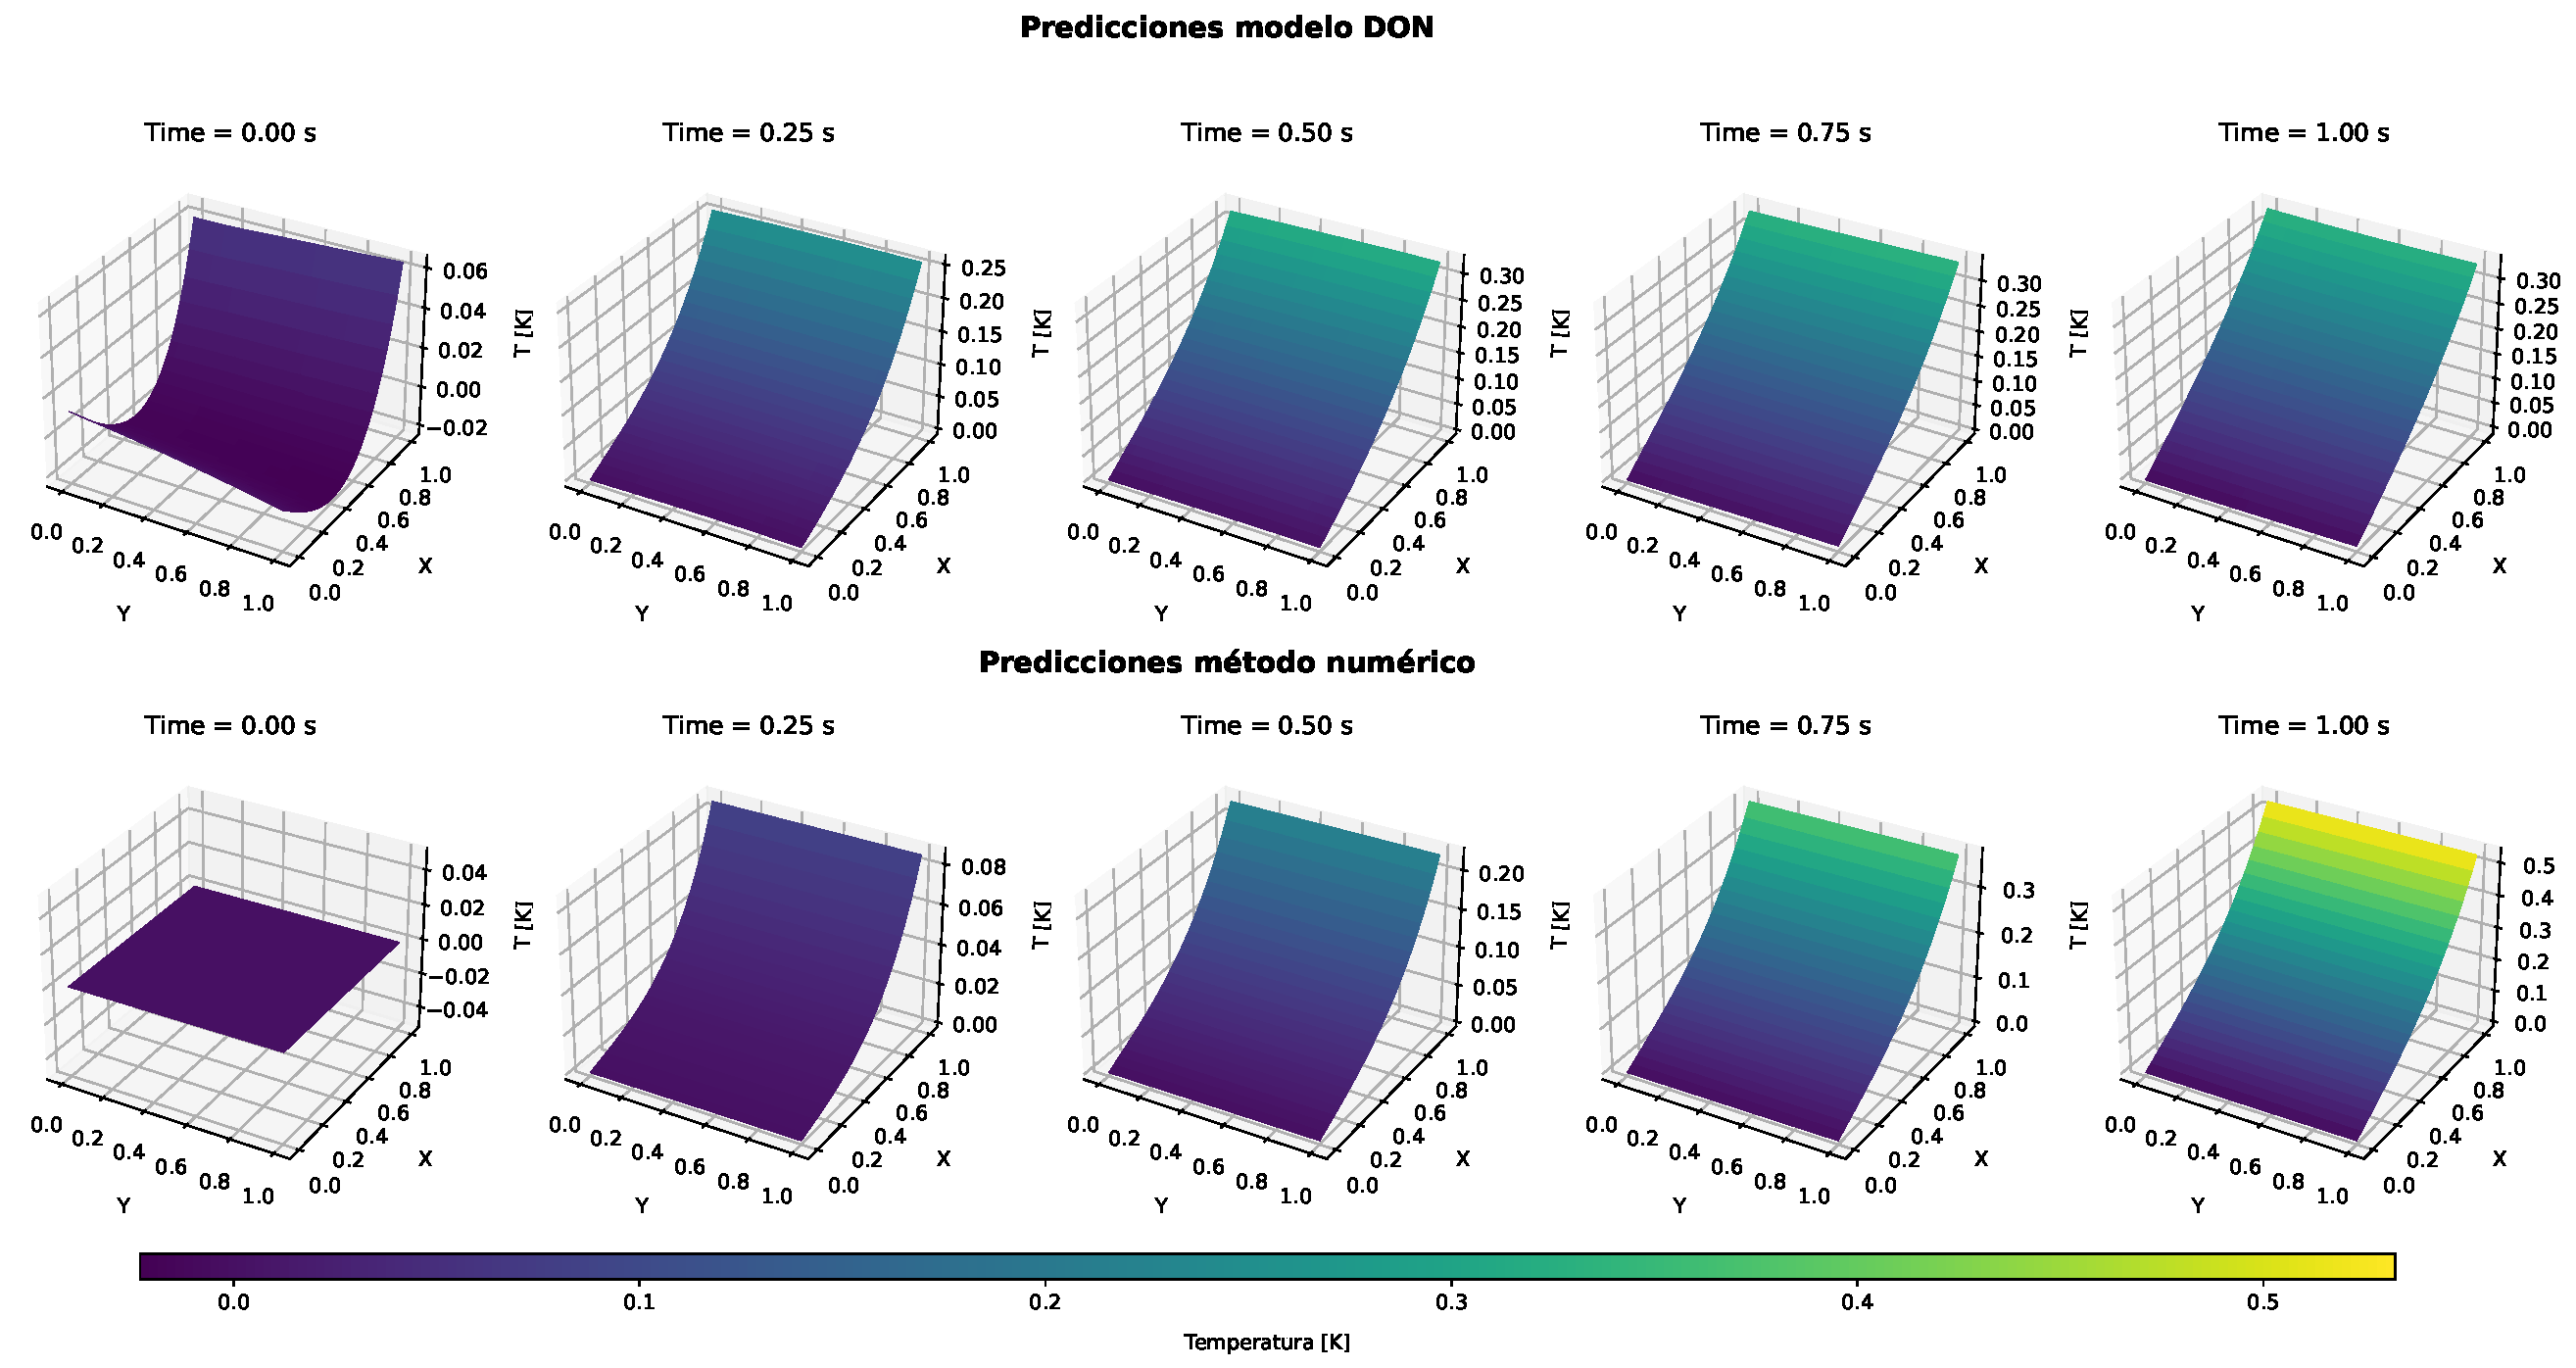
\includegraphics[keepaspectratio]{comparaciones_files/figure-pdf/fig-met-num-vs-model-output-1.pdf}}

}

\caption{\label{fig-met-num-vs-model}Contraste de las predicciones entre
el método de Crank Nikolson y el modelo para cada tiempo.}

\end{figure}%

\section{Validación Cuantitativa frente al Método de
Crank-Nicolson}\label{validaciuxf3n-cuantitativa-frente-al-muxe9todo-de-crank-nicolson}

Para evaluar numéricamente la precisión del modelo DeepONet, se realizó
una comparación sistemática con soluciones de referencia generadas
mediante el método de Crank-Nicolson. Este enfoque proporciona una
métrica objetiva de la exactitud del modelo, siendo complementado con
una serie de gráficos que muestran el error absoluto para cada punto del
dominio en los tiempos de interés.

\begin{Shaded}
\begin{Highlighting}[]
\CommentTok{\# Función para calcular errores}
\KeywordTok{def}\NormalTok{ calculate\_errors(true\_data, pred\_data, times):}
\NormalTok{    results }\OperatorTok{=}\NormalTok{ []}
    
    \ControlFlowTok{for}\NormalTok{ time }\KeywordTok{in}\NormalTok{ times:}
        \CommentTok{\# Filtrar datos por tiempo}
\NormalTok{        true\_subset }\OperatorTok{=}\NormalTok{ true\_data[true\_data[}\StringTok{\textquotesingle{}time\textquotesingle{}}\NormalTok{] }\OperatorTok{==}\NormalTok{ time]}
\NormalTok{        pred\_subset }\OperatorTok{=}\NormalTok{ pred\_data[pred\_data[}\StringTok{\textquotesingle{}time\textquotesingle{}}\NormalTok{] }\OperatorTok{==}\NormalTok{ time]}
        
        \ControlFlowTok{if} \BuiltInTok{len}\NormalTok{(true\_subset) }\OperatorTok{==} \DecValTok{0} \KeywordTok{or} \BuiltInTok{len}\NormalTok{(pred\_subset) }\OperatorTok{==} \DecValTok{0}\NormalTok{:}
            \BuiltInTok{print}\NormalTok{(}\SpecialStringTok{f"Advertencia: No hay datos para tiempo t=}\SpecialCharTok{\{}\NormalTok{time}\SpecialCharTok{\}}\SpecialStringTok{"}\NormalTok{)}
            \ControlFlowTok{continue}
        
        \CommentTok{\# Verificar que las dimensiones coincidan}
        \ControlFlowTok{if} \BuiltInTok{len}\NormalTok{(true\_subset) }\OperatorTok{!=} \BuiltInTok{len}\NormalTok{(pred\_subset):}
            \BuiltInTok{print}\NormalTok{(}\SpecialStringTok{f"Advertencia:Num de puntos no coincide para t=}\SpecialCharTok{\{}\NormalTok{time}\SpecialCharTok{\}}\SpecialStringTok{"}\NormalTok{)}
\NormalTok{            min\_len }\OperatorTok{=} \BuiltInTok{min}\NormalTok{(}\BuiltInTok{len}\NormalTok{(true\_subset), }\BuiltInTok{len}\NormalTok{(pred\_subset))}
\NormalTok{            true\_subset }\OperatorTok{=}\NormalTok{ true\_subset.iloc[:min\_len]}
\NormalTok{            pred\_subset }\OperatorTok{=}\NormalTok{ pred\_subset.iloc[:min\_len]}
        
        \CommentTok{\# Calcular errores para Theta}
\NormalTok{        theta\_true }\OperatorTok{=}\NormalTok{ true\_subset[}\StringTok{\textquotesingle{}Theta\textquotesingle{}}\NormalTok{].values}
\NormalTok{        theta\_pred }\OperatorTok{=}\NormalTok{ pred\_subset[}\StringTok{\textquotesingle{}Theta\textquotesingle{}}\NormalTok{].values}
        
\NormalTok{        absolute\_error }\OperatorTok{=}\NormalTok{ np.}\BuiltInTok{abs}\NormalTok{(theta\_true }\OperatorTok{{-}}\NormalTok{ theta\_pred)}
\NormalTok{        l2\_error }\OperatorTok{=}\NormalTok{ np.sqrt(np.}\BuiltInTok{sum}\NormalTok{((theta\_true }\OperatorTok{{-}}\NormalTok{ theta\_pred)}\OperatorTok{**}\DecValTok{2}\NormalTok{))}
        
\NormalTok{        results.append(\{}
            \StringTok{\textquotesingle{}time\textquotesingle{}}\NormalTok{: time,}
            \StringTok{\textquotesingle{}mean\_absolute\_error\textquotesingle{}}\NormalTok{: np.mean(absolute\_error),}
            \StringTok{\textquotesingle{}max\_absolute\_error\textquotesingle{}}\NormalTok{: np.}\BuiltInTok{max}\NormalTok{(absolute\_error),}
            \StringTok{\textquotesingle{}l2\_error\textquotesingle{}}\NormalTok{: l2\_error}
\NormalTok{        \})}
    
    \ControlFlowTok{return}\NormalTok{ pd.DataFrame(results)}

\CommentTok{\# Calcular errores}
\NormalTok{error\_results }\OperatorTok{=}\NormalTok{ calculate\_errors(crank\_nick\_data, model\_don\_data, times)}

\CommentTok{\# Guardar resultados}
\NormalTok{error\_results.to\_csv(}\StringTok{"data/error\_comparison.csv"}\NormalTok{, index}\OperatorTok{=}\VariableTok{False}\NormalTok{)}
\end{Highlighting}
\end{Shaded}

\begin{table}

\caption{\label{tbl-errores}Error del modelo DeepONet respecto a
Crank-Nicolson.}

\centering{

\begin{verbatim}
|   Tiempo |   MAE |   MaxAE |   Error L2 |
|---------:|------:|--------:|-----------:|
|    0.000 | 0.011 |   0.058 |      0.404 |
|    0.250 | 0.048 |   0.133 |      1.563 |
|    0.500 | 0.032 |   0.058 |      0.934 |
|    0.750 | 0.022 |   0.090 |      0.867 |
|    1.000 | 0.094 |   0.254 |      3.089 |
\end{verbatim}

}

\end{table}%

\subsection{Gráficas de error
absoluto}\label{gruxe1ficas-de-error-absoluto}

\begin{Shaded}
\begin{Highlighting}[]
\CommentTok{\# Calcular el error absoluto entre los dos dataframes}
\NormalTok{error\_data }\OperatorTok{=}\NormalTok{ model\_don\_data.copy()}
\NormalTok{error\_data[}\StringTok{\textquotesingle{}error\textquotesingle{}}\NormalTok{] }\OperatorTok{=}\NormalTok{ np.}\BuiltInTok{abs}\NormalTok{(}
\NormalTok{                    crank\_nick\_data[}\StringTok{\textquotesingle{}Theta\textquotesingle{}}\NormalTok{] }\OperatorTok{{-}}\NormalTok{ model\_don\_data[}\StringTok{\textquotesingle{}Theta\textquotesingle{}}\NormalTok{])}

\CommentTok{\# Crear figura con 3 filas y 2 columnas}
\NormalTok{fig, axes }\OperatorTok{=}\NormalTok{ plt.subplots(nrows}\OperatorTok{=}\DecValTok{1}\NormalTok{, ncols}\OperatorTok{=}\DecValTok{5}\NormalTok{, figsize}\OperatorTok{=}\NormalTok{(}\DecValTok{22}\NormalTok{, }\DecValTok{6}\NormalTok{))}
\NormalTok{axes }\OperatorTok{=}\NormalTok{ axes.ravel()  }\CommentTok{\# Convertir a array 1D para fácil acceso}

\CommentTok{\# Asumir que el grid es regular}
\NormalTok{num\_points }\OperatorTok{=} \BuiltInTok{int}\NormalTok{(np.sqrt(}
\NormalTok{                    error\_data[error\_data[}\StringTok{"time"}\NormalTok{] }\OperatorTok{==}\NormalTok{ times[}\DecValTok{0}\NormalTok{]].shape[}\DecValTok{0}\NormalTok{]}
\NormalTok{                    ))}

\CommentTok{\# Configuración común para los mapas de calor}
\NormalTok{plot\_kwargs }\OperatorTok{=}\NormalTok{ \{}
    \StringTok{\textquotesingle{}cmap\textquotesingle{}}\NormalTok{: }\StringTok{\textquotesingle{}hot\_r\textquotesingle{}}\NormalTok{,}
    \StringTok{\textquotesingle{}shading\textquotesingle{}}\NormalTok{: }\StringTok{\textquotesingle{}auto\textquotesingle{}}\NormalTok{,}
    \StringTok{\textquotesingle{}vmin\textquotesingle{}}\NormalTok{: error\_data[}\StringTok{\textquotesingle{}error\textquotesingle{}}\NormalTok{].}\BuiltInTok{min}\NormalTok{(),}
    \StringTok{\textquotesingle{}vmax\textquotesingle{}}\NormalTok{: error\_data[}\StringTok{\textquotesingle{}error\textquotesingle{}}\NormalTok{].}\BuiltInTok{max}\NormalTok{()}
\NormalTok{\}}
\CommentTok{\# Lista para guardar los gráficos}
\NormalTok{abs\_errors\_pc }\OperatorTok{=}\NormalTok{ []}

\CommentTok{\# Crear los subplots}
\ControlFlowTok{for}\NormalTok{ i, t\_val }\KeywordTok{in} \BuiltInTok{enumerate}\NormalTok{(times):}
\NormalTok{    ax }\OperatorTok{=}\NormalTok{ axes[i]}
    
    \CommentTok{\# Filtrar por tiempo actual}
\NormalTok{    df\_t }\OperatorTok{=}\NormalTok{ error\_data[error\_data[}\StringTok{"time"}\NormalTok{] }\OperatorTok{==}\NormalTok{ t\_val]}
    
    \CommentTok{\# Obtener valores y reshape}
\NormalTok{    X\_vals }\OperatorTok{=}\NormalTok{ df\_t[}\StringTok{"X"}\NormalTok{].values.reshape((num\_points, num\_points))}
\NormalTok{    Y\_vals }\OperatorTok{=}\NormalTok{ df\_t[}\StringTok{"Y"}\NormalTok{].values.reshape((num\_points, num\_points))}
\NormalTok{    error\_vals }\OperatorTok{=}\NormalTok{ df\_t[}\StringTok{"error"}\NormalTok{].values.reshape((num\_points, num\_points))}
    
    \CommentTok{\# Crear mapa de calor}
\NormalTok{    pc }\OperatorTok{=}\NormalTok{ ax.pcolormesh(X\_vals, Y\_vals, error\_vals, }\OperatorTok{**}\NormalTok{plot\_kwargs)}
    
    \CommentTok{\# Configuración de ejes}
\NormalTok{    ax.set\_title(}\SpecialStringTok{f"Tiempo = }\SpecialCharTok{\{}\NormalTok{t\_val}\SpecialCharTok{:.2f\}}\SpecialStringTok{ s"}\NormalTok{, pad}\OperatorTok{=}\DecValTok{10}\NormalTok{)}
\NormalTok{    ax.set\_xlabel(}\StringTok{"X"}\NormalTok{)}
\NormalTok{    ax.set\_ylabel(}\StringTok{"Y"}\NormalTok{)}
\NormalTok{    ax.set\_aspect(}\StringTok{\textquotesingle{}equal\textquotesingle{}}\NormalTok{)}

\NormalTok{    abs\_errors\_pc.append(pc)}

\NormalTok{cbar }\OperatorTok{=}\NormalTok{ fig.colorbar(abs\_errors\_pc[}\OperatorTok{{-}}\DecValTok{1}\NormalTok{], ax}\OperatorTok{=}\NormalTok{axes,}
\NormalTok{                    use\_gridspec}\OperatorTok{=}\VariableTok{True}\NormalTok{, shrink}\OperatorTok{=}\FloatTok{0.9}\NormalTok{,}
\NormalTok{                    aspect}\OperatorTok{=}\DecValTok{90}\NormalTok{, pad}\OperatorTok{=}\FloatTok{0.1}\NormalTok{, orientation}\OperatorTok{=}\StringTok{\textquotesingle{}horizontal\textquotesingle{}}\NormalTok{)}
\NormalTok{cbar.set\_label(}\StringTok{\textquotesingle{}Error absoluto [K]\textquotesingle{}}\NormalTok{)}

\CommentTok{\# Mostrar el gráfico}
\NormalTok{plt.show()}
\end{Highlighting}
\end{Shaded}

\begin{figure}[H]

\centering{

\pandocbounded{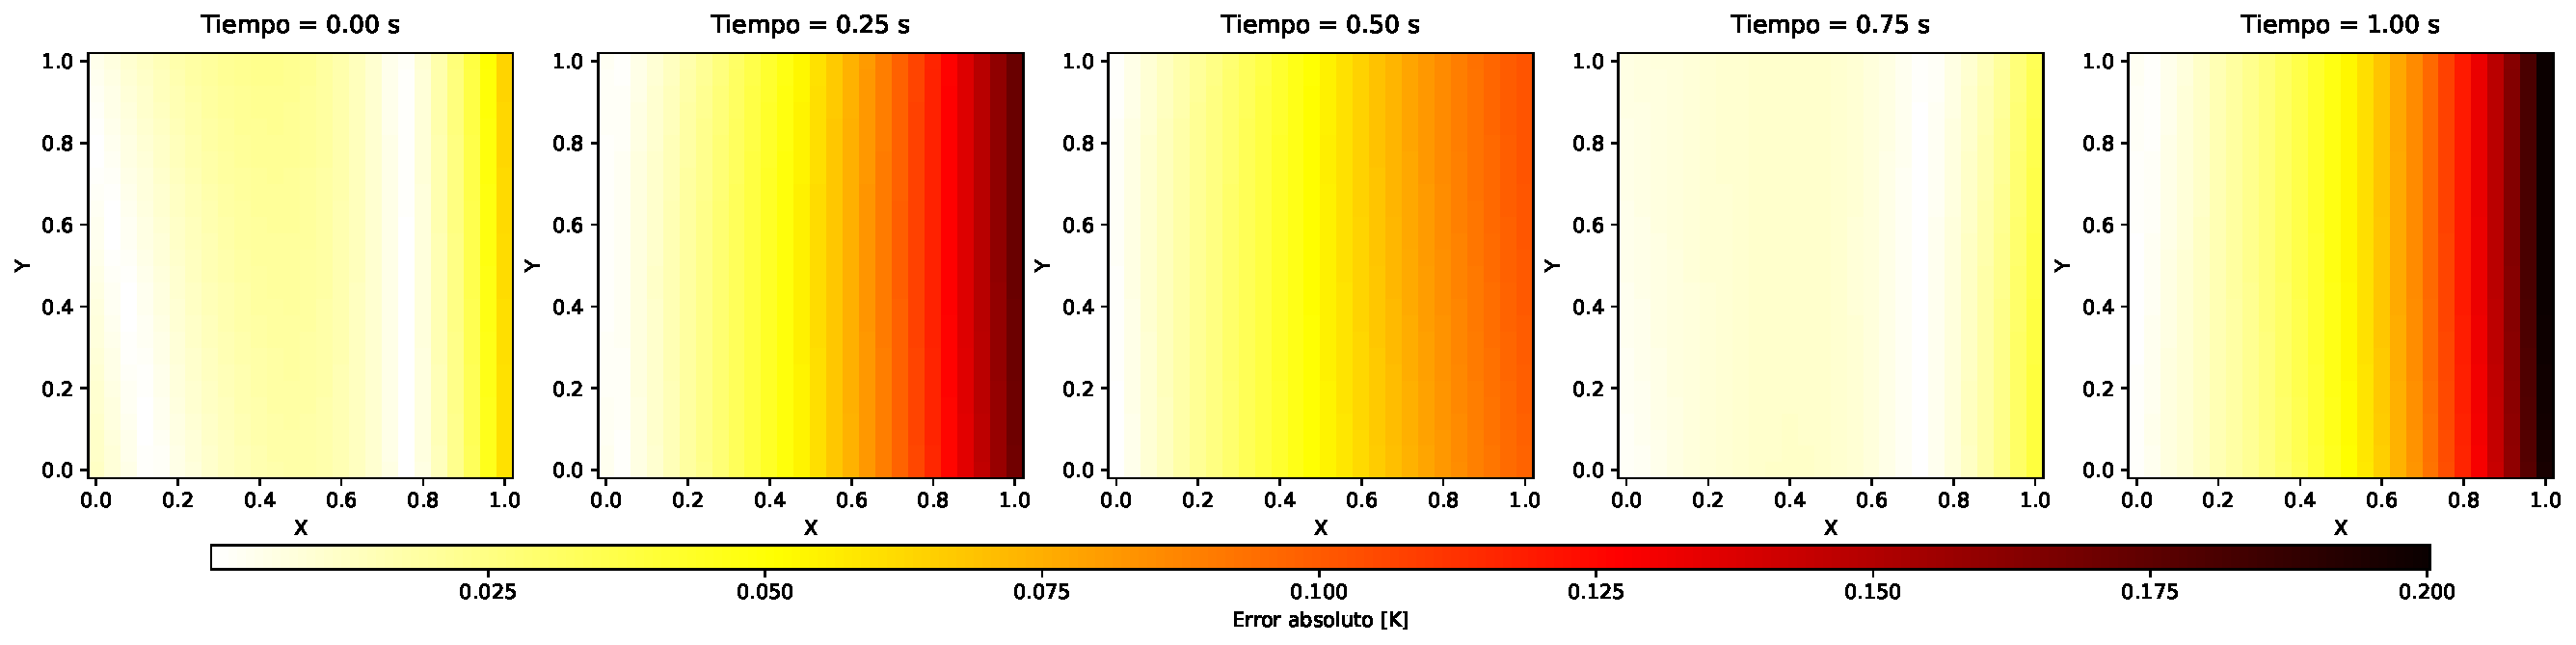
\includegraphics[keepaspectratio]{comparaciones_files/figure-pdf/fig-abs-errors-output-1.pdf}}

}

\caption{\label{fig-abs-errors}Errores absolutos entre el método de
Crank Nikolson y el modelo para cada tiempo.}

\end{figure}%

\bookmarksetup{startatroot}

\chapter{Conclusiones}\label{conclusiones}

El presente trabajo ha abordado la complejidad de resolver una ecuación
diferencial parcial dependiente del tiempo en dos dimensiones espaciales
a través de una red neuronal con la arquitectura DeepONet, asimismo se
obtuvieron predicciones para el cuadrado de \([0,1]\times[0,1]\). Los
hiperparámetros de la red se fueron variando para obtener la mejor
configuración, usando como base los resultados obtenidos por Alessio
Borgi (\citeproc{ref-medical_rep}{2023}). Los resultados obtenidos
mediante la comparación con el método de Crank Nickolson demostraron que
la red neuronal DeepONet se aproxima con un mínimo del 1.1\% y un máximo
del 6.7\% para el error medio absoluto, y cometiendo un error mínimo del
6.4\% y máximo del 20\% para el error máximo absoluto
Tabla~\ref{tbl-errores}.

Los errores obtenidos demuestran la eficacia del modelo para converger a
la condición inicial, pues tal como se aprecia en la
Figura~\ref{fig-abs-errors}, a medida que la ecuación evoluciona en el
tiempo, las predicciones entre el método numérico y la red neuronal
divergen. Aunque esto es probable que se deba a la naturaleza del método
de Crank Nickolson, pues un pequeño error al inicio ocasionaría que
conforme evoluciona la función, ésta cada vez se aleje más del valor
real. Desafortunadamente no se cuenta con una base de datos que sirva
como conjunto de validación por lo que no se puede asegurar que los
resultados del método numérico sean los más óptimos para tomar como
referencia.

Lo anterior evidencia el potencial que tiene las PINNs como herramienta
auxiliar en la solución de ecuaciones diferenciales parciales, pues solo
a través de la definición de la geometria y el espacio temporal (si es
necesario) junto con algunos puntos en el dominio y las condiciones
iniciales y/o de frontera probarón predecir de forma muy acertada el
conjunto de prueba. Ésto representa una gran ventaja respecto a los
modelos de Deep learning que necesitan una gran cantidad de datos para
poder ser entrenados. Otro punto clave de las PINNs es su adaptabilidad
al ruido (\citeproc{ref-karniadakis2021}{George Em Karniadakis 2021})
donde se ha demostrado que incluso a pesar de que los problemas no están
perfectamente bien planteados o si existen parámetros desconocidos la
red puede producir resultados significativos. Siendo ambas situaciones
mencionadas comúnes en el ámbito científico.

Complementado a las PINNs, la arquitectura DeepONet aprende operadores
(mapeos entre espacios de funciones) en lugar de solo aproximar
funciones a diferencia de las PINNs tradicionales, que predicen
soluciones específicas para condiciones fijas, DeepONet es capaz de
generalizar a nuevas condiciones iniciales/frontera sin reentrenamiento,
gracias a su estructura de red dual (branch-trunk). Esto lo hace ideal
para aplicaciones en tiempo real , como la \emph{hipertermia}, donde las
características del problema son suceptibles a cambios, como lo son las
propiedades del cuerpo humano que varían en cada paciente. Un problema
clave que se encontró es que al tener una estructura más compleja, los
tiempos de entrenamiento respectos a las PINNs son mayores, sin embargo
esto se ve bien compensado por su alta capacidad de adaptabilidad a
nuevas condiciones ya sean iniciales o de frontera.

La creación de éste tipo de modelos, tanto PINNs clásicas como DeepONets
se puede ver obstaculizada por el conocimiento en programación del
investigador o estudiante que se plantee programarlos. Si bien tanto el
ámbito científico como en la programación el pensamiento crítico,
seguimiento lógico y abstracción de los problemas son pilares
fundamentales; también es necesario familiarizarse con las librerías que
implementan éste tipo de modelos, además es bastante recomendado tener
una noción básica de como funciona una red neuronal y las partes que la
componen. Lo anterior implica una inversión de tiempo y esfuerzo por
parte de los interesados, cosa que cuando se lleva a cabo un
experiemento o investigación no siempre es posible. Si bien éstas
herramientas son bastante fascinantes y con mucho potencial, como
cualquier nueva habilidad hay que practicar su uso para obtener
resultados que valgan la pena.

Cabe mencionar que las apicaciones de las PINNs son tan amplias como lo
es en sí en campo de las PDEs, si nos centramos únicamente en la
medicina, está la \emph{hipertermia} como tratamiento oncológico, la
cual busca elevar la temperatura en tejidos tumorales (39-45°C) para
potenciar terapias como radioterapia. Sin embargo, controlar la
distribución térmica en tiempo real es un desafío. Las redes neuronales,
especialmente DeepONet, permiten predecir la temperatura de forma rápida
y precisa bajo distintas condiciones, optimizando la dosificación de
calor y minimizando daños a tejidos sanos. Esto facilita terapias
personalizadas y no invasivas, mejorando la eficacia clínica.

\bookmarksetup{startatroot}

\chapter{Futuros trabajos de
investigación}\label{futuros-trabajos-de-investigaciuxf3n}

De cara al futuro es planteable mejorar el modelo siendo más rigurosos
en ciertos aspectos como lo son:

\begin{itemize}
\item
  Ajustar la configuración del optimizador \emph{L-BFGS} ya sea
  aumentando o disminuyendo sus iteraciones máximas, su umbral de
  tolerancia o máximo número de funciones a evaluar.
\item
  Utilizar el modulo de \emph{callbacks} para hacer un
  \emph{earlyStopping} del modelo para evitar un sobreajuste.
\item
  Utilizar un conjunto de validación con datos reales tomados de una
  sesión de hipertérmia.
\item
  Utilizar otro método numérico para comparar el modelo, como puede ser
  diferencias finitas.
\item
  Comparar otras librerías en Python que implementen PINNs como lo son
  SimNet, PyDEns, NeuroDiffEq o SciANN.
\item
  Comparar con otros lengujes de programación como lo es Julia,
  librerías que implementen PINNs como lo son NeuralPDE o ADCME.
\end{itemize}

\bookmarksetup{startatroot}

\chapter*{Referencias}\label{referencias}
\addcontentsline{toc}{chapter}{Referencias}

\markboth{Referencias}{Referencias}

\phantomsection\label{refs}
\begin{CSLReferences}{1}{0}
\bibitem[\citeproctext]{ref-medical_rep}
Alessio Borgi, Alessandro De Luca, Eugenio Bugli. 2023. {«{BioHeat
PINNs: Temperature Estimation with Bio-Heat Equation using
Physics-Informed Neural Networks}»}.
\url{https://github.com/alessioborgi/BioHeat_PINNs/tree/main?tab=readme-ov-file\#bioheat-pinns-temperature-estimation-with-bio-heat-equation-using-physics-informed-neural-networks}.

\bibitem[\citeproctext]{ref-blechs2021}
Blechschmidt, Jan, y Oliver G. Ernst. 2021. {«Three ways to solve
partial differential equations with neural networks---A review»}.
\emph{GAMM-Mitteilungen} 44 (2): e202100006.
\url{https://doi.org/10.1002/gamm.202100006}.

\bibitem[\citeproctext]{ref-burden2011}
Burden, Richard L., y J. Douglas Faires. 2010. {«Numerical Analysis»}.
En \emph{Numerical Analysis}, 9.ª ed., 259-64. Boston, USA: Brooks Cole.

\bibitem[\citeproctext]{ref-dutta2018}
Dutta, Abhijit, y Gopal Rangarajan. 2018. {«Diffusion in pharmaceutical
systems: modelling and applications»}. \emph{Journal of Pharmacy and
Pharmacology} 70 (5): 581-98. \url{https://doi.org/10.1111/jphp.12885}.

\bibitem[\citeproctext]{ref-karniadakis2021}
George Em Karniadakis, Lu Lu, Ioannis G. Kevrekidis. 2021.
{«Physics-informed machine learning»}. \emph{Nature Reviews Physics} 3
(6): 422-40. \url{https://doi.org/10.1038/s42254-021-00314-5}.

\bibitem[\citeproctext]{ref-nci2021}
Instituto Nacional del Cáncer. 2021. {«{¿Qué es el cáncer?}»}
\url{https://www.cancer.gov/espanol/cancer/naturaleza/que-es}.

\bibitem[\citeproctext]{ref-kumar2024deeponet}
Kumar, Varun, Somdatta Goswami, Katiana Kontolati, Michael D. Shields, y
George Em Karniadakis. 2024. {«Synergistic Learning with Multi-Task
DeepONet for Efficient PDE Problem Solving»}. \emph{arXiv preprint
arXiv:2408.02198}. \url{https://arxiv.org/abs/2408.02198}.

\bibitem[\citeproctext]{ref-lu2021deeponet}
Lu, Lu, Pengzhan Jin, Guofei Pang, Zhongqiang Zhang, y George Em
Karniadakis. 2021. {«Learning nonlinear operators via DeepONet based on
the universal approximation theorem of operators»}. \emph{Nature Machine
Intelligence} 3 (3): 218-29.
\url{https://doi.org/10.1038/s42256-021-00302-5}.

\bibitem[\citeproctext]{ref-deepxde}
Lu, Lu, Xuhui Meng, Zhiping Mao, y George Em Karniadakis. 2021.
{«{DeepXDE}: A deep learning library for solving differential
equations»}. \emph{SIAM Review} 63 (1): 208-28.
\url{https://doi.org/10.1137/19M1274067}.

\bibitem[\citeproctext]{ref-hyperthermia}
National Cancer Institute. 2021. {«{Hyperthermia to Treat Cancer}»}.
\url{https://www.cancer.gov/about-cancer/treatment/types/hyperthermia}.

\bibitem[\citeproctext]{ref-omscancer}
Organización Mundial de la Salud. 2022. {«{Cáncer}»}.
\url{https://www.who.int/es/news-room/fact-sheets/detail/cancer}.

\bibitem[\citeproctext]{ref-pennes1948}
Pennes, H. H. 1948. {«Analysis of Tissue and Arterial Blood Temperatures
in the Resting Human Forearm»}. \emph{Journal of Applied Physiology} 1
(2): 93-122. \url{https://doi.org/10.1152/jappl.1948.1.2.93}.

\bibitem[\citeproctext]{ref-quintero2017}
Quintero, Luis A., Mauricio Peñuela, Armando Zambrano, y Edwin
Rodríguez. 2017. {«Optimización del proceso de preparación de soluciones
madre de antibióticos en un servicio farmacéutico hospitalario»}.
\emph{Revista Cubana de Farmacia} 50 (2): 448-65.
\url{https://www.medigraphic.com/cgi-bin/new/resumen.cgi?IDARTICULO=75483}.

\bibitem[\citeproctext]{ref-yang2014}
Yang, Lihong, Xin Wu, Qian Wan, Jian Kong, Rui Liu, y Xiaoxi Liu. 2014.
{«Pharmaceutical preparation of antibiotics: a review on formulation and
technique»}. \emph{Asian Journal of Pharmaceutical Sciences} 9 (3):
145-53. \url{https://doi.org/10.1016/j.ajps.2014.04.001}.

\bibitem[\citeproctext]{ref-zill2008}
Zill, Dennis G., y Michael R. Cullen. 2008. {«Differential Equations
with Boundary-Value Problems»}. En, 7.ª ed., 433-42. Belmont, CA:
Cengage Learning.

\end{CSLReferences}




\end{document}
